\documentclass{styles/tthesis}

\newcommand{\dspic}{dsPIC$^{\text{\textregistered}}$ DSC}
\newcommand{\dcbus}{DC-BUS\texttrademark }

% change the reference to the desired frontpage
\renewcommand{\frontpagefile}{frontpages/frontpage-unipv.inc}

\title{The FELIX project for the \\High Luminosity era of \\the Large Hadron Collider}
\author{Mario Shehu}
\graduation{Master Degree in Computer Engineering}
\academicyear{2024/2025}
\supervisor{
Prof. Tullio Facchinetti \\
Co-supervisor: \\
PhD. Carlo Alberto Gottardo \\
PhD. Jonas Till Roemer \\
}

%-------------------------------------------------------------------
\begin{document}
%-------------------------------------------------------------------

%-------------------------------------------------------------------
% Frontpage
%-------------------------------------------------------------------

% All "variable" data in the frontpage are set using the above commands.
\printfrontpage

%-------------------------------------------------------------------
% Abstract
%-------------------------------------------------------------------

\chapter*{Abstract}

\acl{HEP} experiments conducted at \acs{CERN} will require improvements to the data acquisition systems to meet the challenges posed by the High-Luminosity Large Hadron Collider (\acs{HL-LHC}) era. The thesis introduces the \acs{FELIX} project, detailing its role within the \acs{ATLAS} experiment and the \acl{T-DAQ} infrastructure. It provides an overview of the hardware, firmware, and software developments, emphasizing the context for the personal contributions.\\
Personal contributions include the development of software for the new \acl{ITk} Detector in \acs{ATLAS}, used to perform the reconfiguration of radiation-affected electronics. Additionally, a monitoring system was developed to track the \acs{FELIX} software. The work also involved testing and assembling prototype hardware developed and built for the \acl{HL-LHC}.

The results of tests and benchmarks have been performed to validate the proposed solutions. The thesis concludes with an overview of ongoing research and future developments.

\clearpage
\chapter*{Prefazione}

Gli esperimenti di fisica ad alte energie condotti al \acs{CERN} richiederanno miglioramenti nei sistemi di acquisizione dati per affrontare le sfide poste dall'era ad alta luminosità dell'acceleratore di particelle \acs{LHC}.\\
La tesi introduce il progetto \acs{FELIX}, descrivendo il suo ruolo all'interno dell'esperimento \acs{ATLAS} e dell'infrastruttura di Trigger e Acquisizione Dati. Fornisce una panoramica degli sviluppi hardware, firmware e software, enfatizzando il contesto dei contributi personali.\\
I contributi personali includono lo sviluppo di software per il nuovo rivelatore \acl{ITk} nell'esperimento \acs{ATLAS}, utilizzato per la riconfigurazione dell'elettronica affetta da radiazioni. Inoltre, è stato sviluppato un sistema di monitoraggio per tracciare il software \acs{FELIX}. Il lavoro ha anche coinvolto il collaudo e l'assemblaggio di prototipi hardware sviluppati e costruiti per l'\acl{HL-LHC}.

I risultati di test e benchmark sono stati eseguiti per validare le soluzioni proposte. La tesi si conclude con una panoramica delle ricerche in corso e degli sviluppi futuri.

\chapter*{\mbox{}}

\begin{flushright}
\thispagestyle{empty}
\null\vspace*{\stretch{1}}
{\it “The computer was born to solve problems that did not exist before.”

\vspace{10pt}
— Bill Gates
}
\vspace{\stretch{2}}\null
\end{flushright}
%
\thispagestyle{empty}
\mbox{}
\newpage

%-------------------------------------------------------------------
% Acknowledgments
%-------------------------------------------------------------------

\chapter*{Acknowledgments}

First, I am thankful to my wife, \teexttt{Natalie}, for her love, patience and support, that makes me feel like the Super Mario of the proposal, that can overcome anything, even a "buggy" Bowser. Nothing expands deeper than the ocean, faster than space, and inexorably like time, other than my love for you.\\
Thanks to my brother, Ibrahim, to whom, as the older brother, I hope to be a good example; he is always there for me, like a construction site for an old man.
Thanks to my friends and colleagues Carlo and Jonas, for their help in writing the thesis, for making every problem look solvable, but especially for making every day a little bit lighter and more fun. 
Thanks to Simone who is able to find a place to sit for lunch. Without you I would be hungry every day.\\
In general thanks to all my collegues at CERN, it is a pleasure and an honor to work with you all.\\
Thanks to my supervisor, Professor Tullio Facchinetti, for his guidance and feedback on the thesis.\\
I would like to give an honorable mention to Professor Marco Porta, who supervised a previous thesis project that, although never completed, I still remember fondly and still talk about the driving on racing track. For the same reason my thanks go to Cristiano Resta and Gianfranco Rotondo from GuidaSicura Quattroruote.\\
To all my friends and family, who have studied with me or have supported me in my studies and career, I am grateful for your encouragement and belief.\\

\thispagestyle{empty}
\mbox{}
\newpage


%-------------------------------------------------------------------
% Indexes
%-------------------------------------------------------------------

\tableofcontents
\listoffigures
\listoftables

\mainmatter

% %-------------------------------------------------------------------
\chapter*{Acronyms}
%-------------------------------------------------------------------

\begin{acronym}
\acro{ALICE}{A Large Ion Collider Experiment}
\acro{API}{Application Programming Interface}
\acro{ASIC}{Application Specific Integrated Circuit}
\acro{ATLAS}{A Toroidal LHC ApparatuS}
\acro{BCID}{Bunch Crossing ID}
\acro{BNL}{Brookhaven National Laboratory}
\acro{CERN}{European Organization for Nuclear Research}
\acro{CLOUD}{Cosmics Leaving Outdoor Droplets}
\acro{CMA}{Contiguous Memory Allocation}
\acro{CMS}{Compact Muon Solenoid}
\acro{COTS}{commercial off-the-shelf}
\acro{CTP}{Central Trigger Subsystem}
\acro{DAQ}{Data Acquisition}
\acro{DHCP}{Dynamic Host Configuration Protocol}
\acro{DMA}{Direct Memory Access}
\acro{E-link}{Radiation hard low power electrical link for chip to chip communication}
\acro{ERS}{Error Reporting Service}
\acro{FE}{Front-End}
\acro{FELIX}{Front-End Link eXchange}
\acro{FID}{FELIX identifier}
\acro{FPGA}{Field-Programmable Gate Array}
\acro{GBT}{Gigabit Transceiver}
\acro{HEP}{High Energy Physics}
\acro{HGTD}{High Granularity Timing Detector}
\acro{HL-LHC}{High-Luminosity LHC}
\acro{HTT}{Hardware Tracking for the Trigger}
\acro{IS}{Information Service}
\acro{ISOLDE}{Isotope mass Separator On-Line}
\acro{ITk}{Inner Tracker}
\acro{JTAG}{Joint Test Action Group}
\acro{L0}{Level-0}
\acro{L0Calo}{Level-0 Calorimeter}
\acro{L0Muon}{Level-0 Muon}
\acro{LHC}{Large Hadron Collider}
\acro{LHCb}{Large Hadron Collider beauty}
\acro{LS3}{Long Shutdown 3}
\acro{lpGBT}{Low Power Gigabit Transceiver}
\acro{LTI}{Local Trigger Interface}
\acro{MUCTPI}{Muon-to-Central-Trigger Processor Interface}
\acro{NUMA}{Non-Uniform Memory Access} % a group of processors and memory that are physically and logically grouped together
\acro{OPC}{Open Platform Communication}
\acro{OPC-UA}{OPC Unified Architecture}
\acro{OPCUA-SCA}{OPC-UA Slow Control Adapter}
\acro{OS}{Operating System}
\acro{PCB}{Printed Circuit Board}
\acro{PCIe}{Peripheral Component Interconnect Express}
\acro{PL}{Programmable Logic}
\acro{RDMA}{Remote Direct Memory Access}
\acro{RoCE}{RDMA over Converged Ethernet}
\acro{RTT}{Round Trip Time}
\acro{SEU}{Single Event Upset}
\acro{SMP}{Symmetric Multiprocessing}
\acro{SoC}{System on Chip}
\acro{STAR}{Single Threaded Asynchronous Reactor}
\acro{T-DAQ}{Trigger and Data Acquisition}
\acro{TeV}{Tera electron Volts}
\acro{TTC}{Timing, Trigger and Control}
\end{acronym}

% \input{chapter_intro.inc}
% \input{chapter_sota.inc}
% \input{chapter_tools.inc}
% \input{chapter_implementation.inc}
% \input{chapter_results.inc}
% \input{chapter_conclusions.inc}

\chapter*{List of Acronyms}

\begin{acronym}[OPCUA-SCA]
\acro{ALICE}{A Large Ion Collider Experiment}
\acro{API}{Application Programming Interface}
\acro{ASIC}{Application Specific Integrated Circuit}
\acro{ATLAS}{A Toroidal LHC ApparatuS}
\acro{BCID}{Bunch Crossing ID}
\acro{BNL}{Brookhaven National Laboratory}
\acro{CERN}{European Organization for Nuclear Research}
\acro{CLOUD}{Cosmics Leaving Outdoor Droplets}
\acro{CMA}{Contiguous Memory Allocation}
\acro{CMS}{Compact Muon Solenoid}
\acro{COTS}{commercial off-the-shelf}
\acro{CTP}{Central Trigger Subsystem}
\acro{DAQ}{Data Acquisition}
\acro{DH}{Data Handler}
\acro{DHCP}{Dynamic Host Configuration Protocol}
\acro{DMA}{Direct Memory Access}
\acro{E-link}{Radiation hard low power electrical link for chip to chip communication}
\acro{ERS}{Error Reporting Service}
\acro{FE}{Front-End}
\acro{FELIX}{Front-End Link eXchange}
\acro{FID}{FELIX identifier}
\acro{FPGA}{Field-Programmable Gate Array}
\acro{GBT}{Gigabit Transceiver}
\acro{HEP}{High Energy Physics}
\acro{HGTD}{High Granularity Timing Detector}
\acro{HL-LHC}{High-Luminosity LHC}
\acro{HTT}{Hardware Tracking for the Trigger}
\acro{IS}{Information Service}
\acro{ISOLDE}{Isotope mass Separator On-Line}
\acro{ITk}{Inner Tracker}
\acro{JTAG}{Joint Test Action Group}
\acro{L0}{Level-0}
\acro{L0Calo}{Level-0 Calorimeter}
\acro{L0Muon}{Level-0 Muon}
\acro{LHC}{Large Hadron Collider}
\acro{LHCb}{Large Hadron Collider beauty}
\acro{LS3}{Long Shutdown 3}
\acro{lpGBT}{Low Power Gigabit Transceiver}
\acro{LTI}{Local Trigger Interface}
\acro{MUCTPI}{Muon-to-Central-Trigger Processor Interface}
\acro{NIC}{Network Interface Card}
\acro{NUMA}{Non-Uniform Memory Access} % a group of processors and memory that are physically and logically grouped together
\acro{OPC}{Open Platform Communication}
\acro{OPC-UA}{OPC Unified Architecture}
\acro{OPCUA-SCA}{OPC-UA Slow Control Adapter}
\acro{OS}{Operating System}
\acro{PCB}{Printed Circuit Board}
\acro{PCIe}{Peripheral Component Interconnect Express}
\acro{PL}{Programmable Logic}
\acro{RDMA}{Remote Direct Memory Access}
\acro{RoCE}{RDMA over Converged Ethernet}
\acro{RTT}{Round Trip Time}
\acro{SEU}{Single Event Upset}
\acro{SMP}{Symmetric Multiprocessing}
\acro{SoC}{System on Chip}
\acro{STAR}{Single Threaded Asynchronous Reactor}
\acro{T-DAQ}{Trigger and Data Acquisition}
\acro{TeV}{Tera electron Volts}
\acro{TTC}{Timing, Trigger and Control}
\end{acronym}

% Example usage in your text:
%\ac{FELIX}   displays the acronym and its expansion on first use, then just the acronym
%\acf{FELIX}  always displays the acronym and its expansion
%\acs{FELIX}  displays only the acronym (short form)
%\acl{FELIX}  displays only the expansion (long form)
\chapter{Introduction}

This document is the result of six months of work at \acs{CERN}, within the \acs{FELIX} project, in the context of the hardware and software upgrades for the \acl{HL-LHC} era.

\section{Motivation}

Modern \acl{HEP} experiments, such as those conducted at \acf{CERN}, produce massive quantities of data, necessitating \acf{DAQ} systems capable of high throughput, high scalability, and low latency. As the \acf{LHC} transitions to its High-Luminosity phase \acs{HL-LHC}, the demands on \acs{DAQ} infrastructure have increased, creating the need for new hardware and software solutions. This thesis addresses these challenges by focusing on the readout part inside a \acl{DAQ} system, specifically, the \acs{FELIX} platform and the network library \texttt{netio3}.

\section{Context}

The \acs{HL-LHC} will deliver a tenfold increase in integrated luminosity\footnote{A measure of the collected data size, defined as the time integral of the instantaneous luminosity, typically expressed in inverse femtobarns (fb\(^{-1}\)).}, and will increase pile-up to as many as 200 collisions per bunch crossing (compared with about 50 today)\footnote{Instantaneous luminosity is the measure of the number of potential collisions per surface unit (or cross section) over a given period of time.} \cite{HighLumiLHC}. This will require new hardware and software solutions to handle over 150 TB/s of data, generated by proton-proton collisions at a rate of 40 million events per second.

Inside the \acl{T-DAQ} infrastructure of the \acs{ATLAS} experiment is the \acs{FELIX} platform, a data router that connects detector electronics with data processing systems by converting detector-specific data transmission protocols into a standard network protocol.
\texttt{netio3} is the network library that powers the networking of the \acs{FELIX} project.\\
The \acs{FELIX} platform itself is divided in three main components: the hardware, the firmware and the software. The hardware consists of a \acs{PCIe} card installed in a server. The firmware runs on a \acs{FPGA} on the card and is responsible for the data acquisition and processing. The software provides an interface for users to interact with the system.

\section{Objectives}

The primary objective of this thesis is to contribute to the development of new features of the \acs{FELIX} readout system, the enhancement and optimization of existing ones, the testing and assembly of the hardware, and a performance evaluation of the entire system ensuring it meets the new requirements.
New features include a way to send configuration data to frontend electronics and a monitoring system.

\section{Thesis Structure}

\begin{itemize}
    \item \textbf{Chapter 2} provides an overview of \acs{CERN}, its experiments and the role of \acs{FELIX}; it presents where we currently are and better details what will be the future requirements.
    
    \item \textbf{Chapter 3} dives into the \acs{FELIX} project in its entirety, detailing the hardware, firmware and software components. At the end of the chapter are the personal contributions to the topic.
    
    \item \textbf{Chapter 4} focuses on the \texttt{felix-star} software suite, detailing its most important components. It also includes the personal contributions to the topic.
    
    \item \textbf{Chapter 5} presents the \texttt{netio3} network library, making a distinction between the backend and frontend part. Personal contributions end the chapter.
    
    \item \textbf{Chapter 6} contains the results of the hardware testing and benchmarking of the FLX-182-1B cards, and the performance evaluation of software.
    
    \item \textbf{Chapter 7} concludes the thesis with a summary of the work done and future developments.
\end{itemize}
\chapter{State of the Art}

\ac{CERN} \cite{cern-homepage} is the world's leading institution in the field of high-energy particle physics. Figure~\ref{fig:science-gateway} is an aerial view of the \acs{CERN} main site located in Meyrin, Geneva.

\begin{figure}[htbp]
\centering
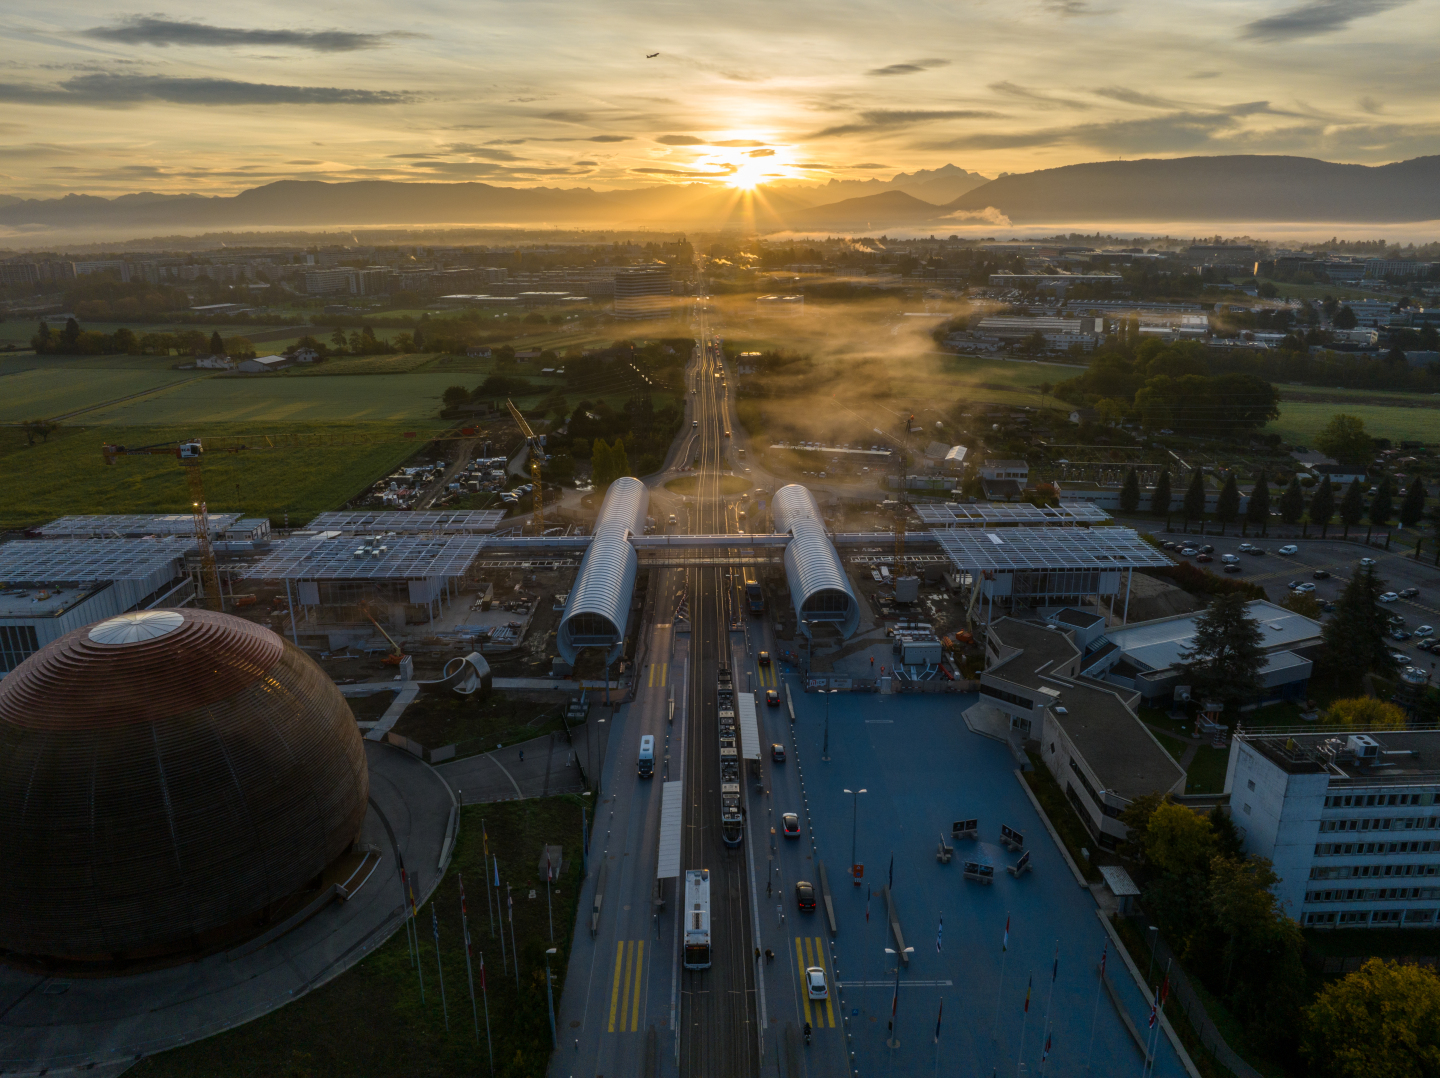
\includegraphics[width=\textwidth]{images/introduction/cern.jpg}
\caption[CERN Science Gateway]{On the left the Globe of Science and Innovation, in the center the CERN Science Gateway designed by Renzo Piano, on the right the blue square is Place des Particules. The rest of CERN's main site develops on the right of Place des Particules \protect\cite{cern_science_gateway}}
\label{fig:science-gateway}
\end{figure}

The \acf{CERN} convention \cite{cern-convention} signed in 1953 declares that its scientific work shall be publicly shared and dedicated to peaceful advancement. At the time of writing, \ac{CERN} comprises 25 member states, with scientists from over 110 countries collaborating to decipher the fundamental structure of the universe.

Situated on the Franco-Swiss border near Geneva, \ac{CERN} hosts a chain of increasingly powerful accelerators and purpose-built detectors that operate at energies mirroring the universe's earliest moments. Major experiments such as \acs{ATLAS} \cite{atlas-experiment}, \acs{CMS} \cite{cms-experiment}, \acs{ALICE} \cite{alice-experiment}, and \acs{LHCb} \cite{lhcb-experiment} rely on the \ac{LHC} \cite{Lebrun:1284331} for their data collection. Meanwhile, projects like \acs{CLOUD} \cite{Kirkby:1310801}, \acs{ISOLDE} \cite{isolde-facility}, and NA62 \cite{Martellotti:2056863} explore complementary aspects of particle physics, expanding our knowledge on the Standard Model, which in short, is our best explanation of how the basic building blocks of matter interact \cite{standard-model}.

Beyond contributions to fundamental science, \ac{CERN} has a rich history of technological innovation, perhaps the most famous example being the creation of the World Wide Web in 1989 \cite{www-proposal}. Advances in data analysis, accelerator technology, and detector development have also impacted fields such as medical imaging, materials science, and network engineering \cite{cern-tech-impact}.

\clearpage
\section{\acs{LHC}}
\label{sec:lhc-experiments}

The \ac{LHC} \cite{Lebrun:1284331, Brüning:782076} is \ac{CERN}'s flagship accelerator and the most powerful particle collider in operation world-wide. Housed in a 27-km circular tunnel roughly 100 meters underground, it accelerates two beams of protons to 99.9999991\% the speed of light and collides them at energies up to 13.6 \ac{TeV}. Figure~\ref{fig:LHC} shows an aerial view with an overlay illustrating the geographic location of the LHC and its major experiments, giving a sense of the scale of the facility.

Particles enter the \ac{LHC} after passing through smaller accelerators (see Figure~\ref{fig:cern-complex}). A beam inside the beam pipes in the \ac{LHC} is not a continuous stream of particles, but is divided into bunches. Bunches typically contain around $10^{11}$ protons, they are spaced 25 ns apart, and collide at a rate of 40 MHz. On average, there are 43 proton-proton collisions on each bunch crossing.

\begin{figure}[htbp]
\centering
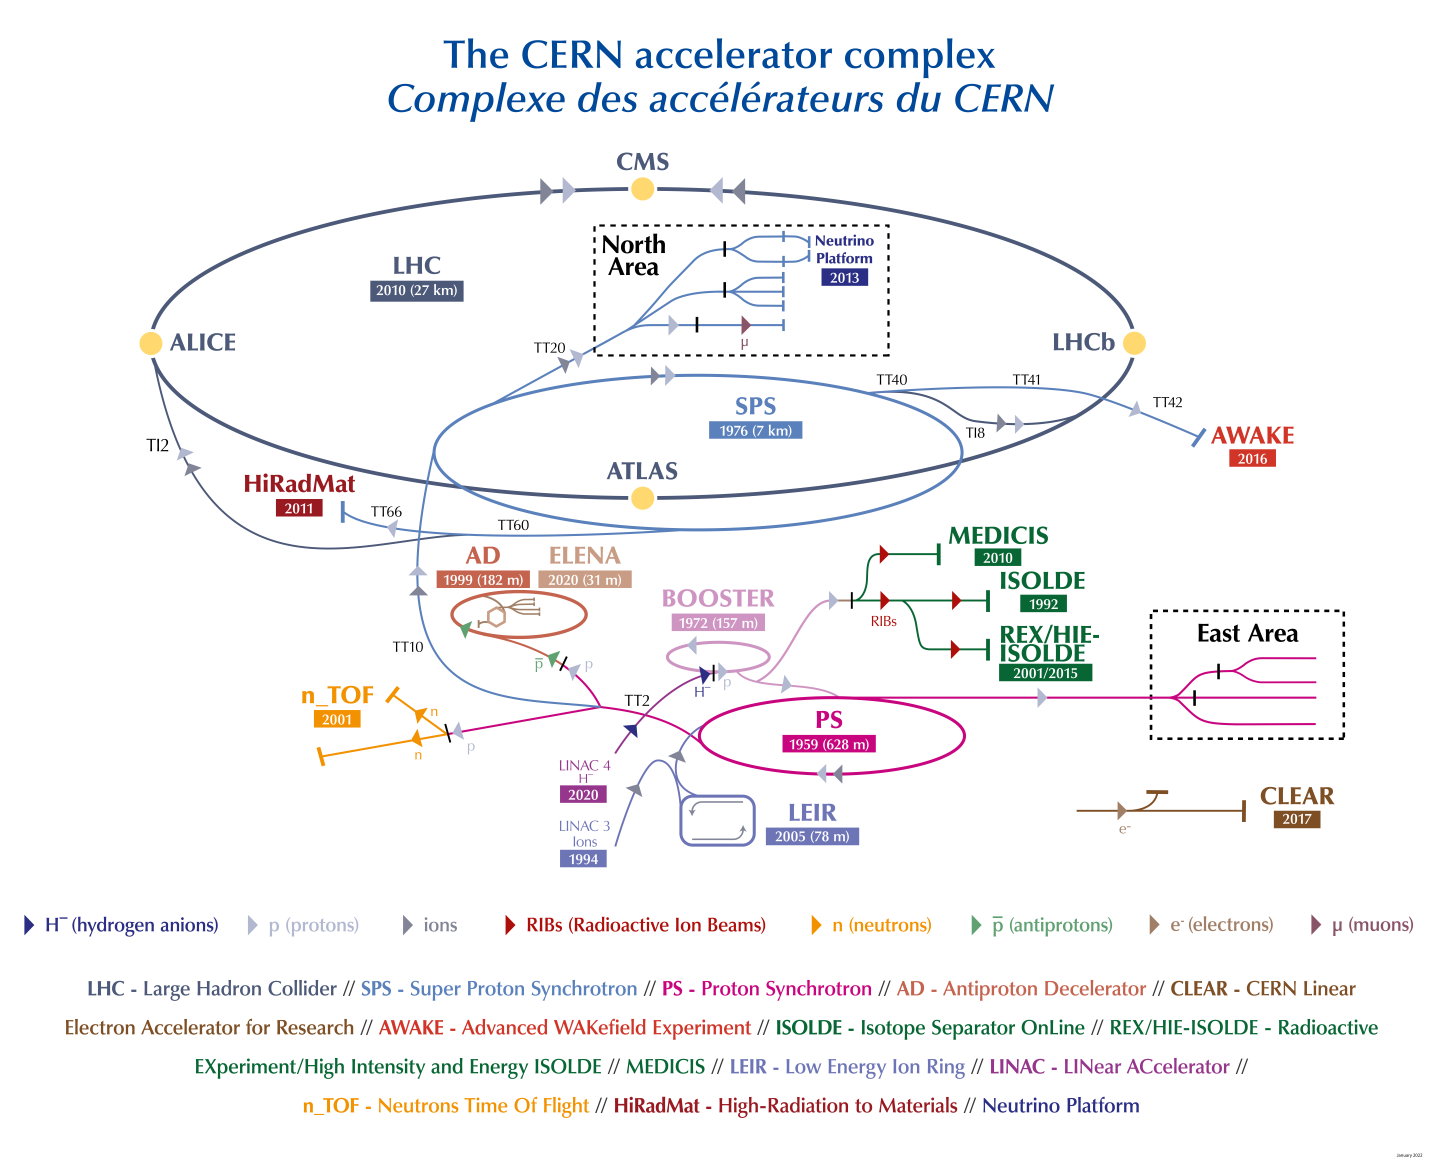
\includegraphics[width=\textwidth]{images/introduction/cern-experiments.png}
\caption[The accelerator complex at CERN]{The accelerator complex at \acs{CERN}. Several smaller accelerators boost the beam before it enters the \acs{LHC}. Primary experiments (\acs{ALICE}, \acs{ATLAS}, \acs{CMS}, \acs{LHCb}) are placed around the \acs{LHC} ring. Image source: \protect\cite{cern_accelerator_complex}}
\label{fig:cern-complex}
\end{figure}

As mentioned before, the data is gathered through four main experiments, located around the \acs{LHC} ring:
\begin{itemize}
    \item \textbf{ATLAS} \cite{atlas-experiment} and \textbf{CMS} \cite{cms-experiment}: General-purpose detectors that investigate the Higgs boson, measure quantities of the Standard Model and search for phenomena beyond it.
    \item \textbf{LHCb} \cite{lhcb-experiment}: Specializes in asymmetries between matter and antimatter, particularly in $b$-quarks. 
    \item \textbf{ALICE} \cite{alice-experiment}: Focuses on the quark-gluon plasma in heavy-ion collisions.
\end{itemize}

Regular Long Shutdowns enable maintenance and upgrades to the \acs{LHC} and its experiments. These planned intervals improve performance and add new features, ensuring the facility meets new scientific objectives, including the transition toward the High-Luminosity \acs{LHC} phase.

\begin{figure}[H]
\centering
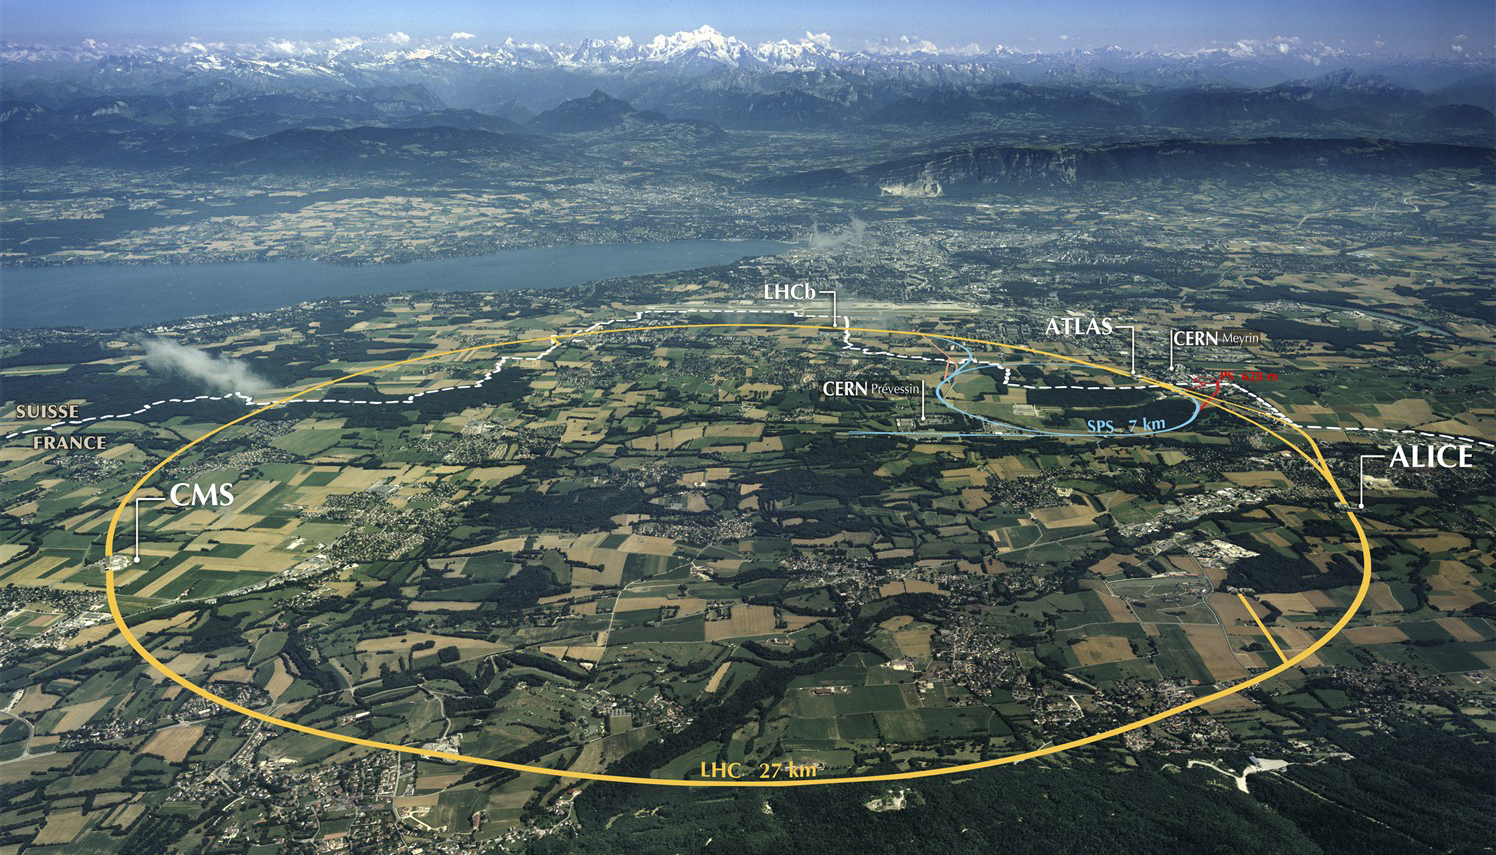
\includegraphics[width=\textwidth]{images/introduction/LHC_map.jpg}
\caption{An approximate overlay of the \acs{LHC}'s underground tunnel. \protect\cite{lhc_tunnel_map}}
\label{fig:LHC}
\end{figure}

\subsubsection{The High-Luminosity \acs{LHC} Era}

\ac{CERN} is preparing for \acf{LS3}, after which the \acs{HL-LHC} era begins around June 2030, as shown in Figure~\ref{fig:LHC-schedule} which displays the schedule up to the year 2041. The \acf{HL-LHC} aims to increase luminosity by an order of magnitude over the original design, enabling data collection at rates of up to 200 simultaneous proton-proton collisions per bunch crossing. This high collision density compels substantial upgrades in \acs{ATLAS} detectors and online systems.

\begin{figure}[H]
\centering
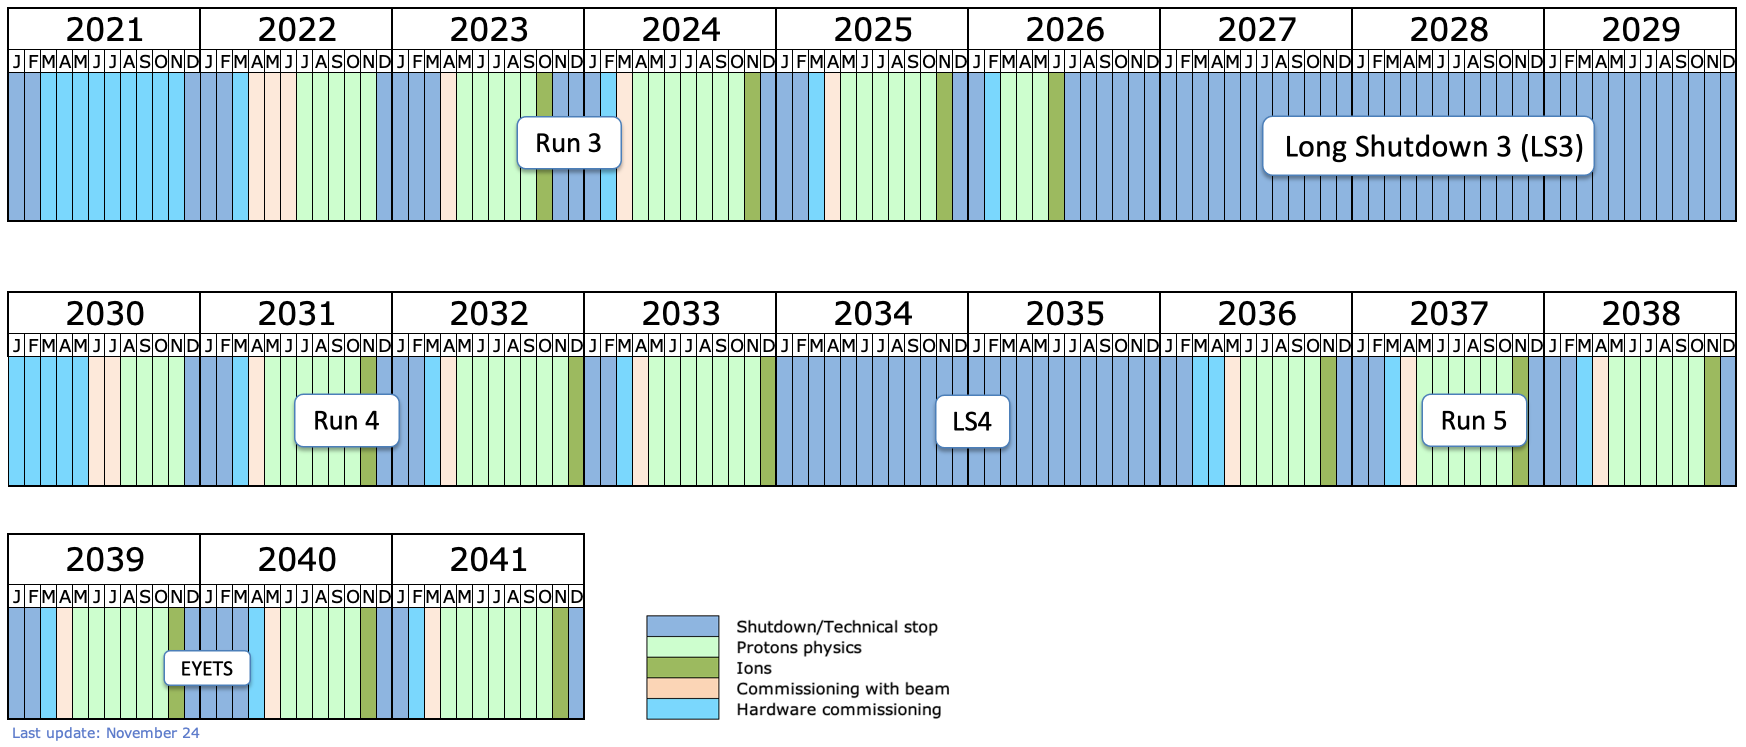
\includegraphics[width=\textwidth]{images/introduction/LHC-schedule.png}
\caption[Upgrade schedule for the LHC]{Upgrade schedule for the LHC. LS3 marks the start of HL-LHC conditions. \protect\cite{lhc_upgrade_schedule}}
\label{fig:LHC-schedule}
\end{figure}

\clearpage
\section{ATLAS Experiment}

The \acs{ATLAS} detector \cite{atlas-experiment} shown in Figures~\ref{fig:atlas-model} and \ref{fig:atlas}, central to this thesis, is the largest general-purpose experiment at the \acs{LHC}. Comparable in size to a multistory building (44 m in length and 25 m in diameter), \acs{ATLAS} features multiple layers of specialized subsystems (detectors), each engineered to measure distinct particle properties. Key scientific goals include precision studies of the Higgs boson (discovered in 2012 \cite{atlas-higgs-discovery}) and searches for supersymmetric particles.

\begin{figure}[H]
\centering
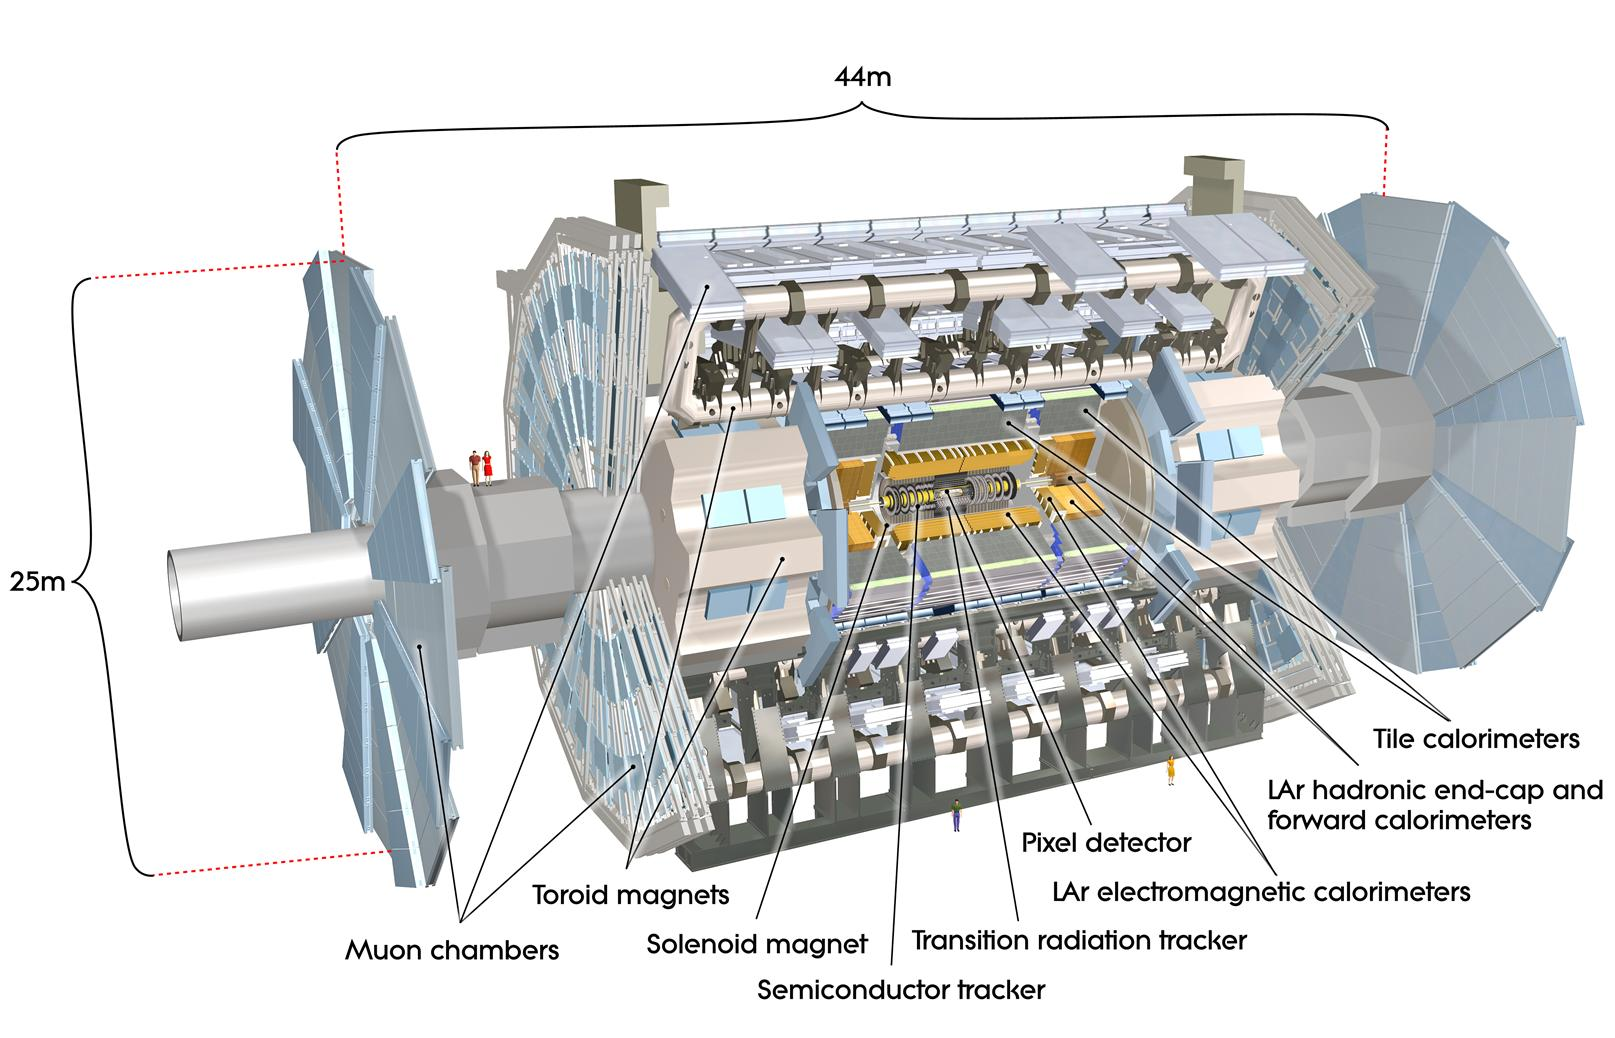
\includegraphics[width=\textwidth]{images/introduction/atlas-model.jpg}
\caption[Schematic of the ATLAS detector]{Schematic of the \acs{ATLAS} detector. Two primary magnet systems bend charged particle trajectories. The detectors measure particle energy and momentum. Image source: \acs{ATLAS} experiment. \protect\cite{atlas-experiment}}
\label{fig:atlas-model}
\end{figure}

Operated by a global collaboration of over 5,000 scientists, \acs{ATLAS} sits about 100 meters below ground. A separate service cavern (USA15) houses cooling and readout electronics, which are connected to the detectors via optical fibers. Because of intense magnetic fields and radiation, the \acs{lpGBT} \acs{ASIC} \cite{lpgbt} has been developed to allow multipurpose high speed bidirectional optical links between the detectors and readout system.

\begin{figure}[H]
\centering
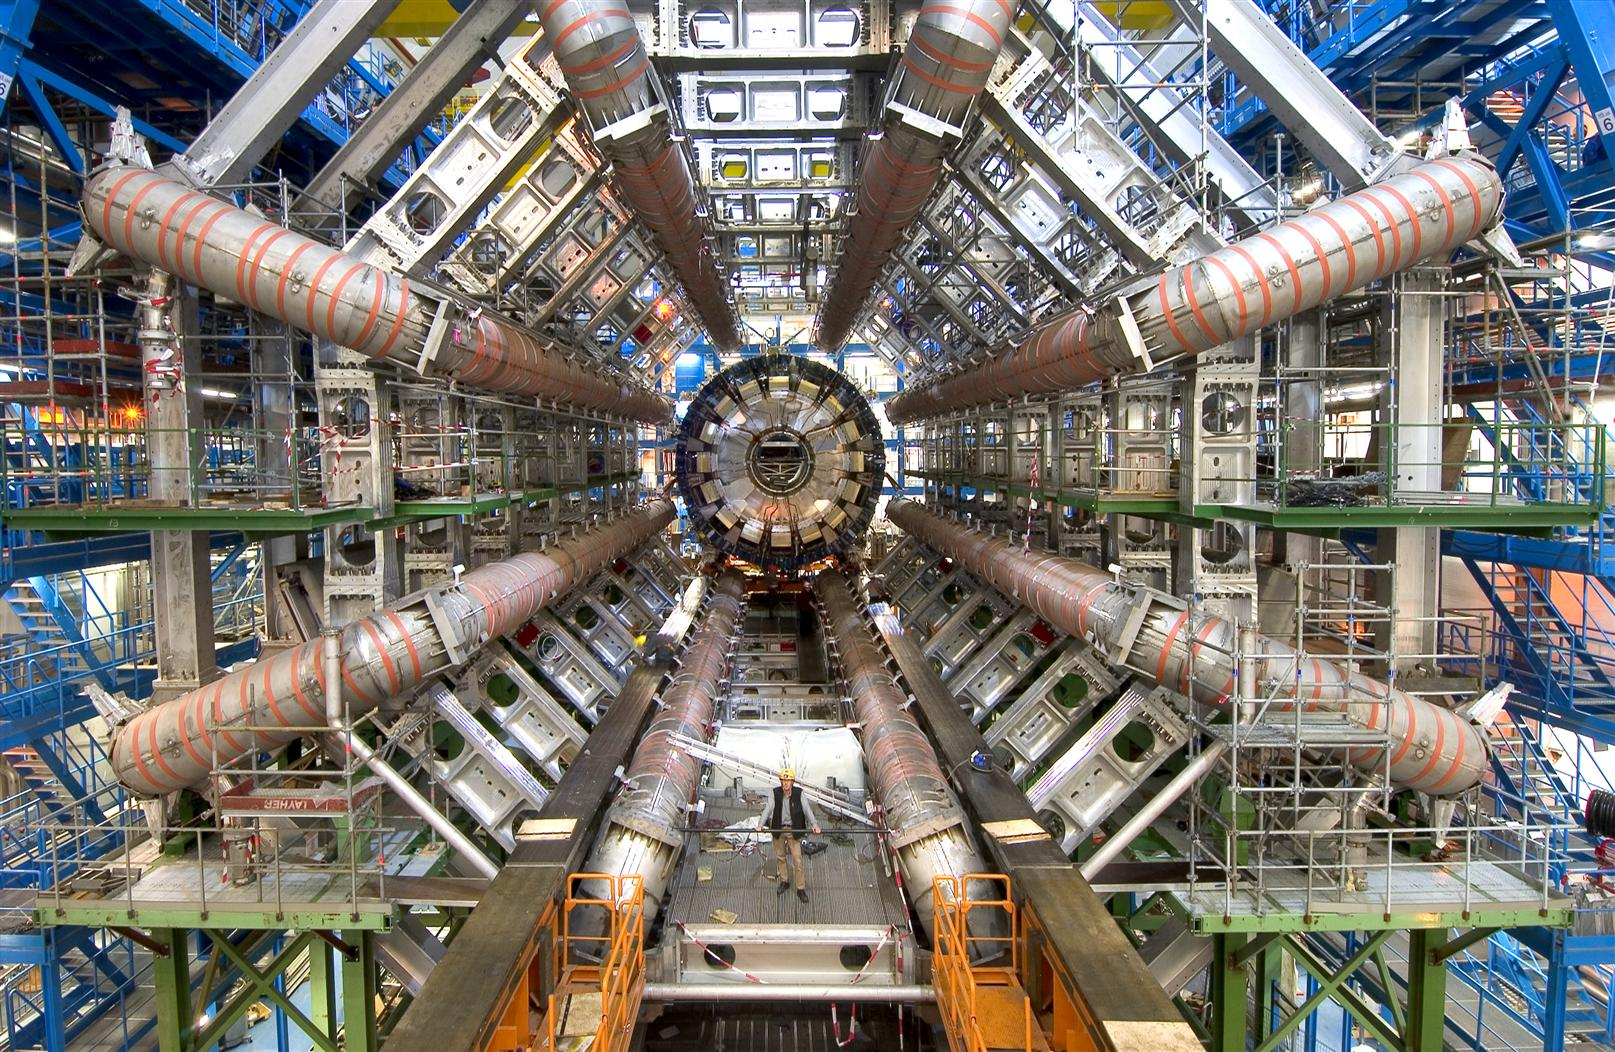
\includegraphics[width=\textwidth]{images/introduction/atlas.jpg}
\caption{A view of the ATLAS detector installation. \protect\cite{atlas-experiment}}
\label{fig:atlas}
\end{figure}

\subsubsection{\acs{ATLAS} Phase II}

The \acs{ATLAS} Phase II upgrade \cite{Affolder:2799535} adapts the experiment to make use of the \acs{HL-LHC}'s higher luminosity. 
More precisely, the \acs{HL-LHC} will deliver 10 times more data compared to the previous run.  To meet the challenges \acs{ATLAS} will include a new \acf{HGTD} \cite{hgtd-phase2-upgrade} for a better time measurement, a new all-silicon \acf{ITk} \cite{atlas-itk-pixel-detector}, and a new \acs{T-DAQ} system capable of handling data arriving at 1 MHz.

\clearpage
\section{\acf{T-DAQ}}

As the name suggests, the \acs{ATLAS} \acf{T-DAQ} system is composed of a Trigger and a \acf{DAQ} system. Figure~\ref{fig:tdaq} provides a high level description of the \acs{T-DAQ} architecture showing the Detectors layer and the Event Filter layer at the bottom. A more in-depth description of each architectural component is presented below.

\begin{figure}[htbp]
\centering
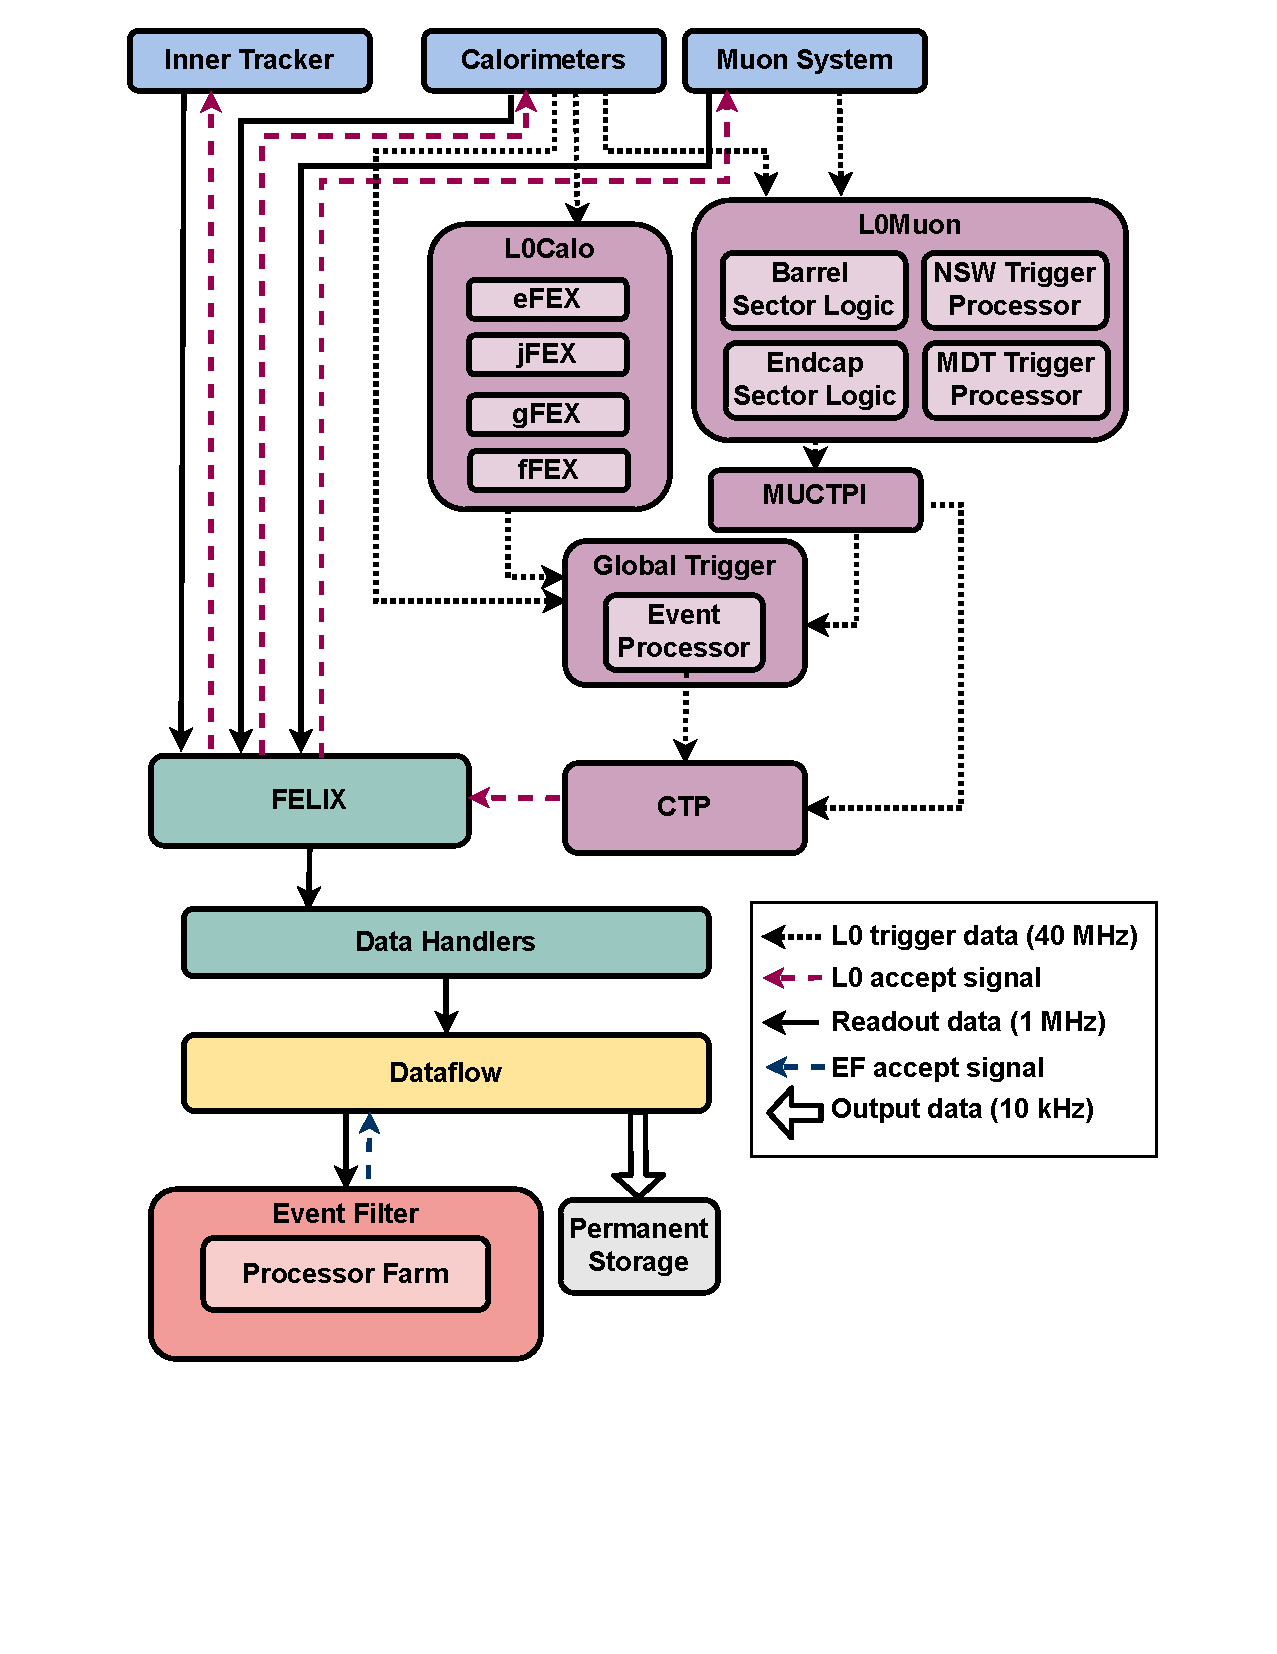
\includegraphics[width=0.68\textwidth]{images/introduction/Baseline_TDAQ_Phase-II_Architecture.pdf}
\caption[Overview of the T-DAQ architecture]{An overview of the \acs{T-DAQ} architecture is shown. The three main layers are color-coded: the Level-0 Trigger in pink, the DAQ subsystem (comprising the Readout and Dataflow subsystems) in green and yellow, and the Event Filter at the bottom in red. The detectors, shown in blue, are not part of the T-DAQ infrastructure but are included to provide context on how T-DAQ interfaces with other components of the \acs{ATLAS} experiment.}
\label{fig:tdaq}
\end{figure}

\subsection{Trigger}

\begin{definition}
\label{def:event}
An event captures the hits generated by a collision in a bunch crossing observed by detectors.
\end{definition}

This can reach data volumes of roughly 60 TB/s. The duty of triggers is to filter out non-interesting events.

\begin{definition}
\label{def:trigger}
A trigger is a hard- or software-based filter that issues \emph{ACCEPT} or \emph{REJECT} decisions for each event.
\end{definition}

Triggers may examine particle counts, reconstructed energy, momenta, or other indicators of interesting physics.

The Trigger layer that forms a first-level hardware based trigger includes \cite{tdaq} \acs{L0Calo}, \acs{L0Muon} (\acs{L0} stands for Level 0, which is a term used for components detached from the main detector that perform a first filtering of the events), the Global Trigger, and the Central Trigger Subsystem (\acs{CTP}). Essentially, \acs{L0Calo} filters for the energies and positions of charged and neutral particles, \acs{L0Muon} is used to filter for muons, and the \acs{MUCTPI}'s task is to interface \acs{L0Muon} with \acs{CTP}. The Global Trigger \cite{tdaq} uses full-granularity calorimeter information to perform offline-like algorithms, refines the trigger objects calculated by \acs{L0Calo} and \acs{L0Muon}, calculates event-level quantities, and executes topological algorithms. The \acs{CTP} \cite{tdaq} forms triggers based on combinations of inputs or conditions received from the Global Trigger and other sources; it applies pre-scale factors and introduces deadtime when necessary to avoid saturation in the front-end and readout systems. Ultimately, it makes the final decision on whether the event is accepted, driving the \acs{TTC} network to start the readout process of the detectors.

\subsection{\acs{DAQ} - Readout and Dataflow}
\label{subsec:daq}

\begin{definition}
\label{def:daq}
A data acquisition system \acs{DAQ} aggregates detector data, relays trigger outcomes, and writes all accepted events to permanent storage.
\end{definition}

Figure~\ref{fig:tdaq} shows that the Data Handler can receive data only from the \acs{FELIX} card \cite{tdaq}, also the \acs{FELIX} card is directly linked to the Detectors via an optical interface, other than the \acs{L0} Triggers. The \acs{FELIX} card receives data fragments from the detectors, sends them to the Data Handlers that re-organizes those fragments for detector-specific operations that will be performed by the Dataflow.

The Dataflow system \cite{tdaq} includes all components needed to aggregate the data fragments towards a full event-building, to buffer the events for the software trigger (Event Filter) and send the selected event to permanent storage.

\subsection{Event Filter}

The Event Filter system \cite{tdaq} consists of a CPU-based processing farm. The \acs{EF} system runs more elaborate algorithms that take the data from the entire detector to reduce the trigger rate by another order of magnitude to get it down to the final output rate of 10 KHz. Events will be rejected as early as possible during their processing. The Event Filter decisions will be communicated to the Dataflow, which will then transfer the accepted events to permanent storage.

\clearpage
\section{\acs{FELIX}}

Within the \acs{T-DAQ} architecture, \acs{FELIX} offers an interface between detector front-end electronics and downstream data processing. It is designed to handle the high data rates projected for the forthcoming HL-LHC phase and allows for a flexible, high-throughput readout system.

\subsubsection{\acs{FELIX} in Phase II}

\begin{figure}[H]
\centering
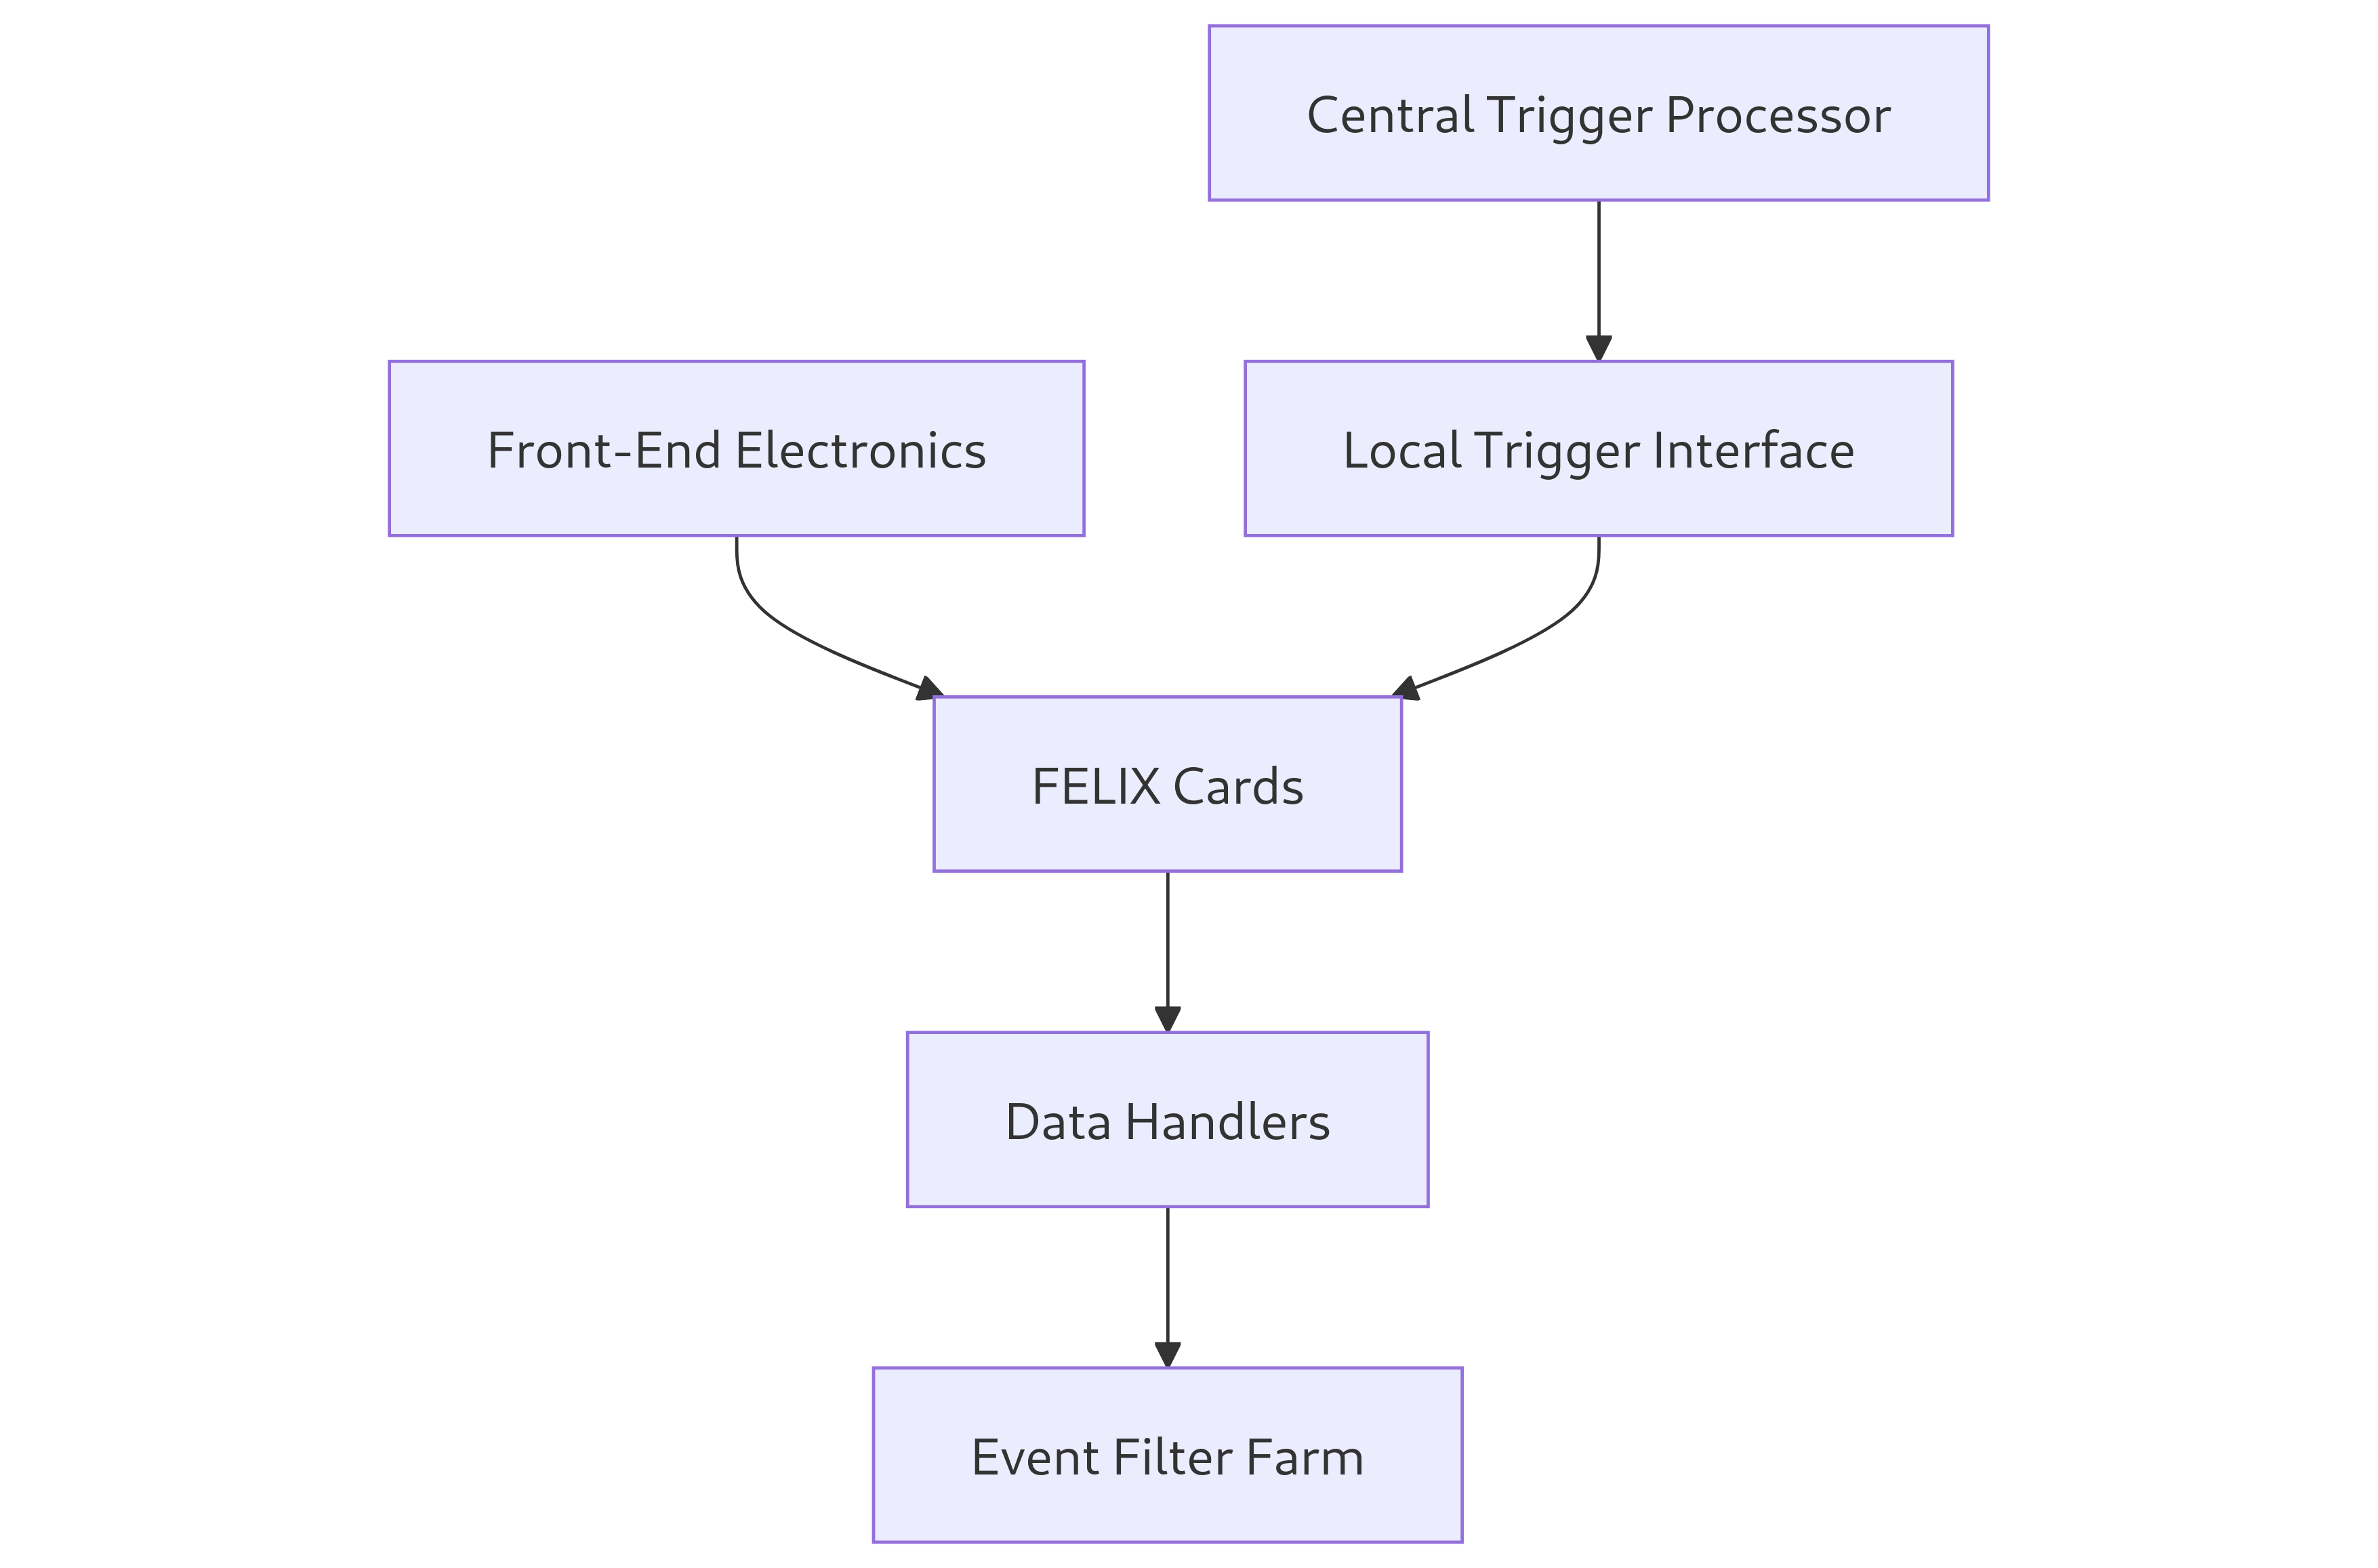
\includegraphics[width=\textwidth]{images/introduction/felix-block-diagram.png}
\caption[Block diagram of the Readout system]{Block diagram of the Readout system, focusing on the FELIX part. It is connected to Front-End Electronics, Data Handler, Event Filter Farm, and \acf{LTI}.}
\label{fig:felix-block-diagram}
\end{figure}

\acs{FELIX} readout system will be linking upgraded front-end electronics to commercial servers through \acs{FPGA}-based \acs{PCIe} cards. It will be translating detector-specific protocols into standard network packets, allowing the detectors to communicate with the Data Handlers.\\
This last part is the main answer of why \acs{FELIX} is needed in the \acs{T-DAQ} architecture. On-detector electronics must be radiation tolerant. For this purpose at \acs{CERN} have been developed custom electronics, like \acl{lpGBT} \cite{lpgbt} that uses its own protocol, but the rest of the underlying architecture uses normal network protocols since they are shielded from radiations; \acs{FELIX} is in between the two layers allowing them to communicate. Also \acs{FELIX} is necessary for distributing the clock signal of the \acs{LHC} to the front-end electronics.\\
The new \acs{FELIX} system can handle event rates in excess of 1 MHz and data streams beyond 5~TB/s\footnote{The entire system composed of many servers can handle such data rate, not per single component}, and allows for:
\begin{itemize}
    \item \textbf{Scalability}: Commodity server hardware reduces the cost and simplifies maintenance compared to purely custom designs.
    \item \textbf{System Flexibility}: Uniform support for various upgraded detector systems, including the new \acs{ITk} detector and \acs{HGTD}.
    \item \textbf{Low-Latency}: Low latency and minimal data loss are important to reach the \acs{HL-LHC} objectives.
\end{itemize}

\subsubsection{Scale and Implementation of the \acs{FELIX} System}

As briefly explained before (Subsection~\ref{subsec:daq}) the \acs{ATLAS} Phase-II Readout System is responsible for collecting data from all detector subsystems and preparing it for processing by the Dataflow and Event Filter layers. It is made up of two main parts: \acs{FELIX} and the \acf{DH}.

\paragraph{FELIX.}
\acf{FELIX} acts as the bridge between the detector front-end electronics and the computing infrastructure. It connects directly to the detectors through high-speed optical links and converts their data into a format that can be handled by standard network equipment.

Each \acs{FELIX} server is equipped with two custom \acs{PCIe} cards (FLX-155), which will be described in detail in Section~\ref{subsec:FLX-155}. Each FLX-155 card is built around an AMD Versal \acs{FPGA} and supports up to 48 optical links. The actual number of active links depends on the specific detector and its bandwidth requirements. For instance, the \acs{ITk} Strips detector uses 1,824 10~Gb/s optical links, distributed across 76 FELIX cards, each being a 24-links card.

Once the data is received, \acs{FELIX} uses a high-speed 200~Gb/s network interface to send it to the next stage: the Data Handler servers.

\paragraph{Data Handlers.}
The Data Handlers are a set of dedicated servers that receive data from \acs{FELIX} and perform two main tasks. First, they aggregate data into larger "fragments" by combining data that belongs to the same event. Then, they pass those fragments to the Dataflow system for further processing.

Depending on the detector, the \acs{DH} may work in two different modes. For some detectors—like \acs{ITk}, \acs{HGTD}, and New Small Wheel \cite{nsw}, the data arrives in small pieces from many sources, and the \acs{DH} must perform "fragment building." This requires more computing power, as it involves grouping, formatting, and validating the data. For other detectors that already send pre-formatted fragments, the \acs{DH} simply acts as a relay.

\paragraph{Infrastructure and Constraints.}
The entire Readout System will be installed in the USA15 underground counting room, which has some limits on available space and cooling. There are 36 server racks available, each with a 15~kW power budget.

In total, the system will include:
\begin{itemize}
    \item 783 \acs{FELIX} cards (including spares),
    \item 371 \acs{FELIX} servers (2 cards per server),
    \item 701 Data Handler servers.
\end{itemize}

Together, these components consume around 495~kW of power, filling all available racks.



\chapter{\acs{FELIX} project}

The first goal of the \acs{FELIX} project is to replace diverse, custom-made hardware readout solutions with a unified platform that relies on \acf{COTS} components. With this approach, tasks once handled by such custom hardware are now managed by software modules that subscribe to \acs{FELIX} cards inside off-the-shelf servers.

From an architectural perspective, \acs{FELIX} is built around a custom \acs{PCIe} card installed in a host server. Incoming data from detector front-ends reaches system memory via \acf{DMA}. Software on the host then distributes these data streams to network-connected clients.\\
Bidirectional communication is supported, allowing data to flow from software back to the front-end electronics. The \texttt{netio3} network library allows using TCP/IP if needed, in addition to \acf{RoCE} as a supported network protocol. This chapter examines the \acs{FELIX} project covering its hardware, firmware and software design.

\clearpage
\section{Hardware}

Three hardware implementations are currently relevant:

\begin{itemize}
    \item \textbf{FLX-182}: used for prototyping and testing new features;
    
    \item \textbf{FLX-155}: candidate card for \acs{ATLAS} Phase-II operations and an upgrade over FLX-182;
    
    \item \textbf{FLX-712}: older version developed for Phase-I, used in production, but no longer under development or used for testing new features.
\end{itemize}

\subsection{FLX-182}

The FLX-182 \cite{Ilic:2873569} (Figure \ref{fig:FLX-182-combined}) is a Phase-II prototype card developed by \acf{BNL}. It features:

\begin{itemize}
    \item AMD Versal Prime VP-1802 \acf{SoC}
    \item FireFly optical transceivers supporting up to 24 duplex links at 25 Gb/s \cite{firefly-optical-transceiver}
    \item \acf{LTI} interface (Figure~\ref{fig:ALTI} shows the \acs{ATLAS} \acl{LTI})
    \item Electrical trigger interface
    \item \acs{PCIe} Gen4 connectivity
\end{itemize}

\begin{figure}[htbp]
\centering
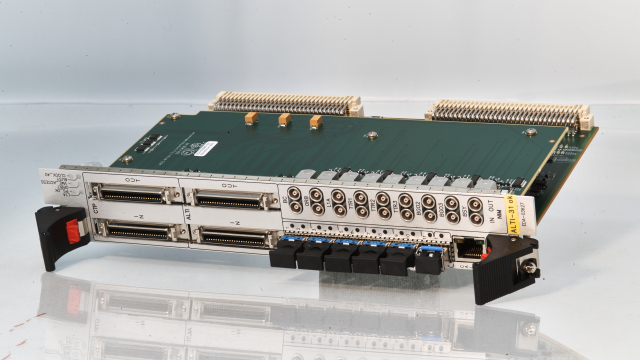
\includegraphics[width=\textwidth]{images/felix/lti.jpg}
\caption[ATLAS Local Trigger Interface]{The ATLAS \acl{LTI} is a replacement of the legacy \acf{TTC}.\\ \texttt{Timing}: Distribution of the \acs{LHC} bunch clock (the same clock source for entire system).\\\texttt{Trigger}: Decision from the trigger system indicating whether the data for a given event should be sent to the readout.\\ \texttt{Control}: Sends synchronization/configuration commands, subdetectors raise a Busy signal to indicated that the internal buffers are filling up.\\Image source \protect\cite{alti}.}
\label{fig:ALTI}
\end{figure}

This card requires a 16-lane \acs{PCIe} slot (preferably Gen4) configured with x8x8 bifurcation. Power is supplied through a \acs{PCIe} 6+2 pin cable, and the card's form factor necessitates two adjacent \acs{PCIe} slots for bracket installation. 
The operating system is PetaLinux. The OS and the \acl{PL} image for the \acs{FPGA} are embedded into a micro-SD card. The \acs{PL} can be reprogrammed by either updating the SD card contents or using the onboard \ac{JTAG} controller, accessible via the USB-C port on the front panel.

\begin{figure}[H]
\centering
\begin{subfigure}[b]{0.48\textwidth}
    \centering
    \includegraphics[width=\textwidth]{images/felix/felix-front-panel.png}
    \caption{FLX-182 front panel.}
    \label{fig:FLX-182-panel}
\end{subfigure}
\hfill
\begin{subfigure}[b]{0.48\textwidth}
    \centering
    \includegraphics[width=\textwidth]{images/felix/FLX-182.png}
    \caption{FLX-182 top view.}
    \label{fig:FLX-182}
\end{subfigure}
\caption{FLX-182 hardware.}
\label{fig:FLX-182-combined}
\end{figure}

\subsection{FLX-155}
\label{subsec:FLX-155}
The FLX-155 (Figure \ref{fig:FLX-155}) is the designated candidate for \acs{ATLAS} Phase-II operations, with advancement over the FLX-182 prototype like the support for a more recent \acs{PCIe} standard, and double the number of optical transceiver links. Its specifications include:

\begin{itemize}
    \item AMD Versal Premium VP-1552 SoC
    \item Support for up to 48 duplex links rated at up to 25 Gb/s via FireFly optical transceivers
    \item \acs{PCIe} Gen5 connectivity
    \item \acs{LTI} interface via a dedicated FireFly B04 module
    \item Optional 400 GbE interface capability (not utilized in ATLAS)
\end{itemize}

The FLX-155 will be 1cm shorter than the FLX-182 and will require similar installation parameters: a 16-lane \acs{PCIe} slot (preferably Gen5) with x8x8 bifurcation configuration. At least one \acs{PCIe} 6+2 pin power cable is required. Like its predecessor, the FLX-155 is equipped with an SD card containing both the PetaLinux operating system and \acl{PL} images.

\begin{figure}[H]
\centering
\begin{subfigure}[b]{0.7\textwidth}
    \centering
    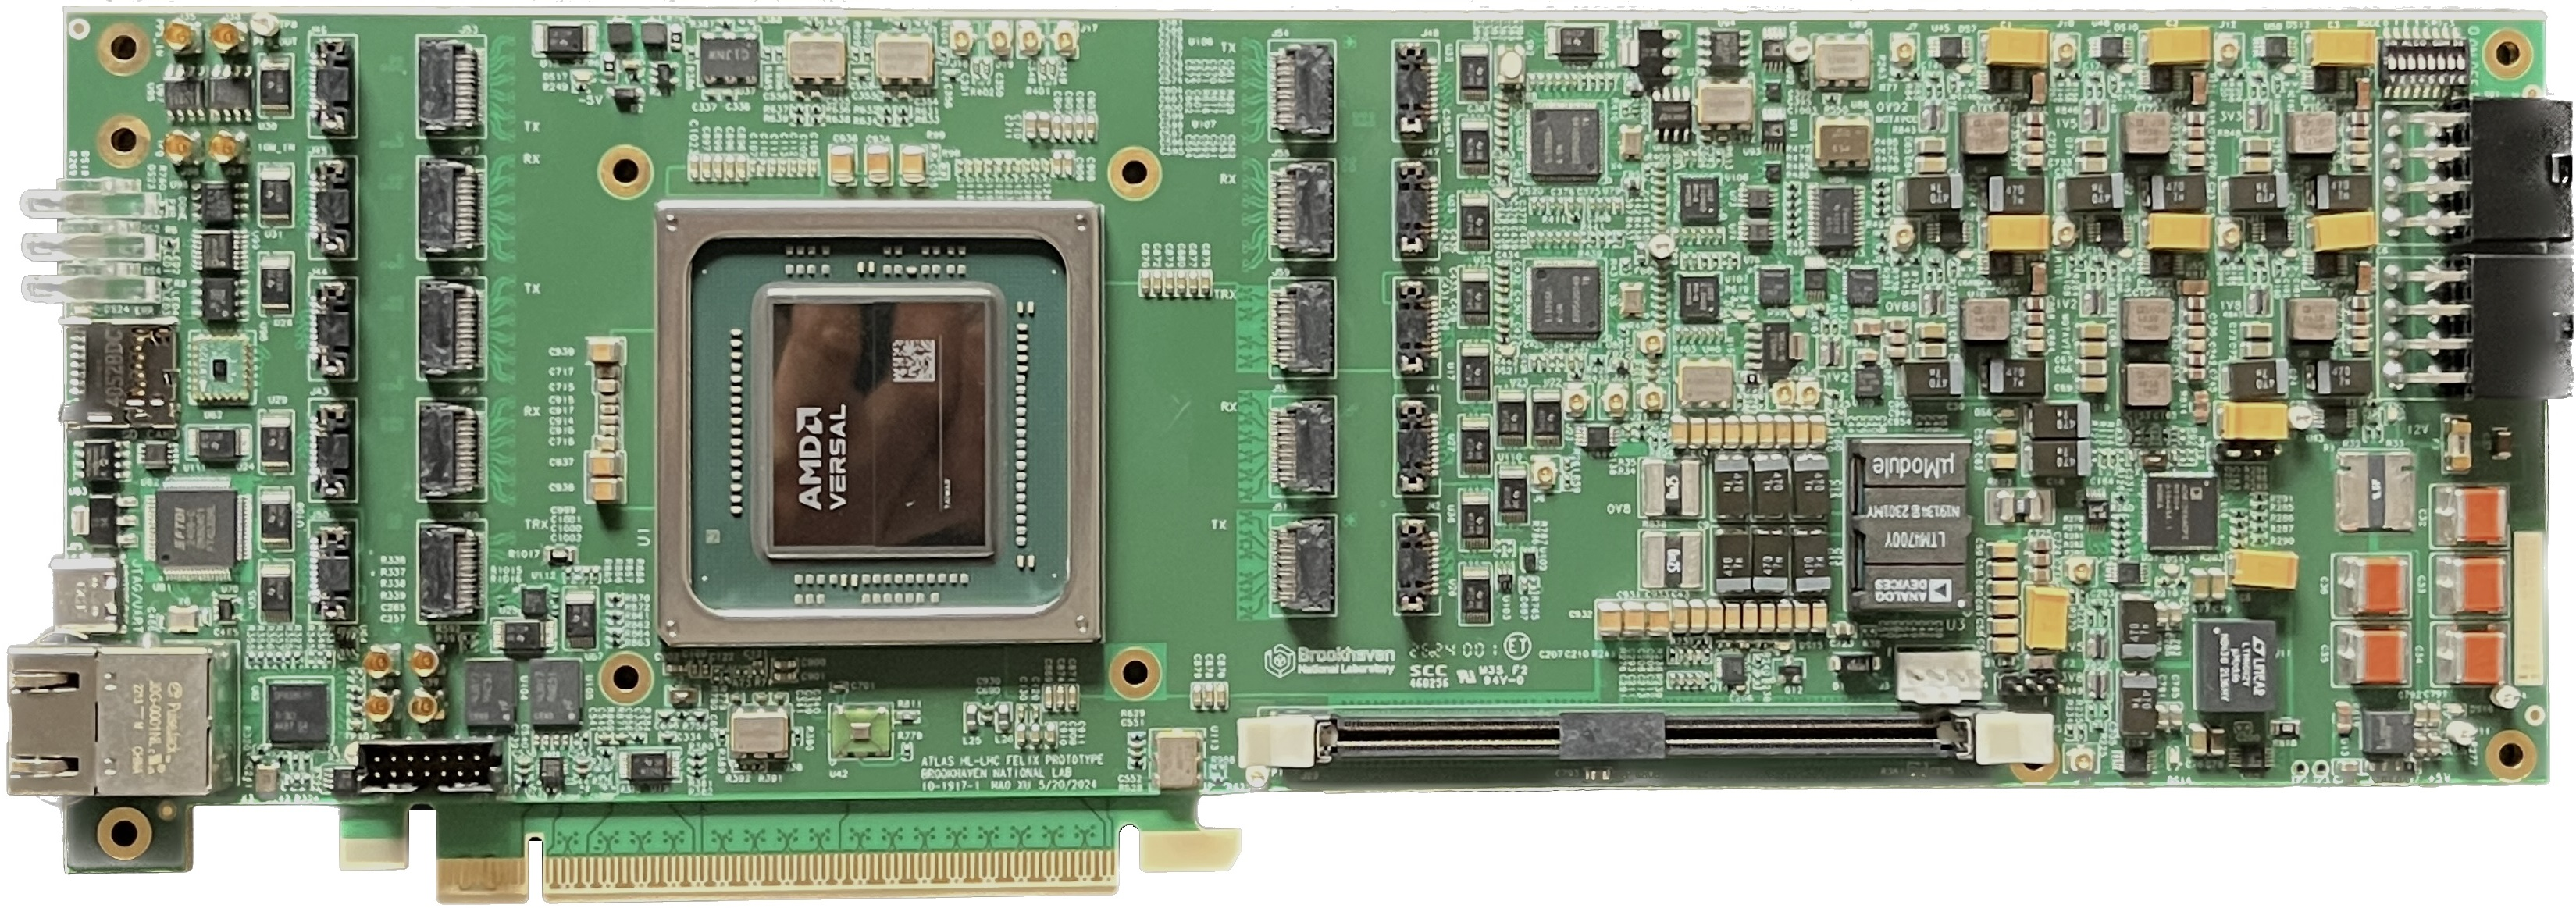
\includegraphics[width=\textwidth]{images/felix/flx155_top.jpg}
    \caption{FLX-155 front view.}
    \label{fig:FLX-155-top}
\end{subfigure}

\vspace{0.2cm}

\begin{subfigure}[b]{0.7\textwidth}
    \centering
    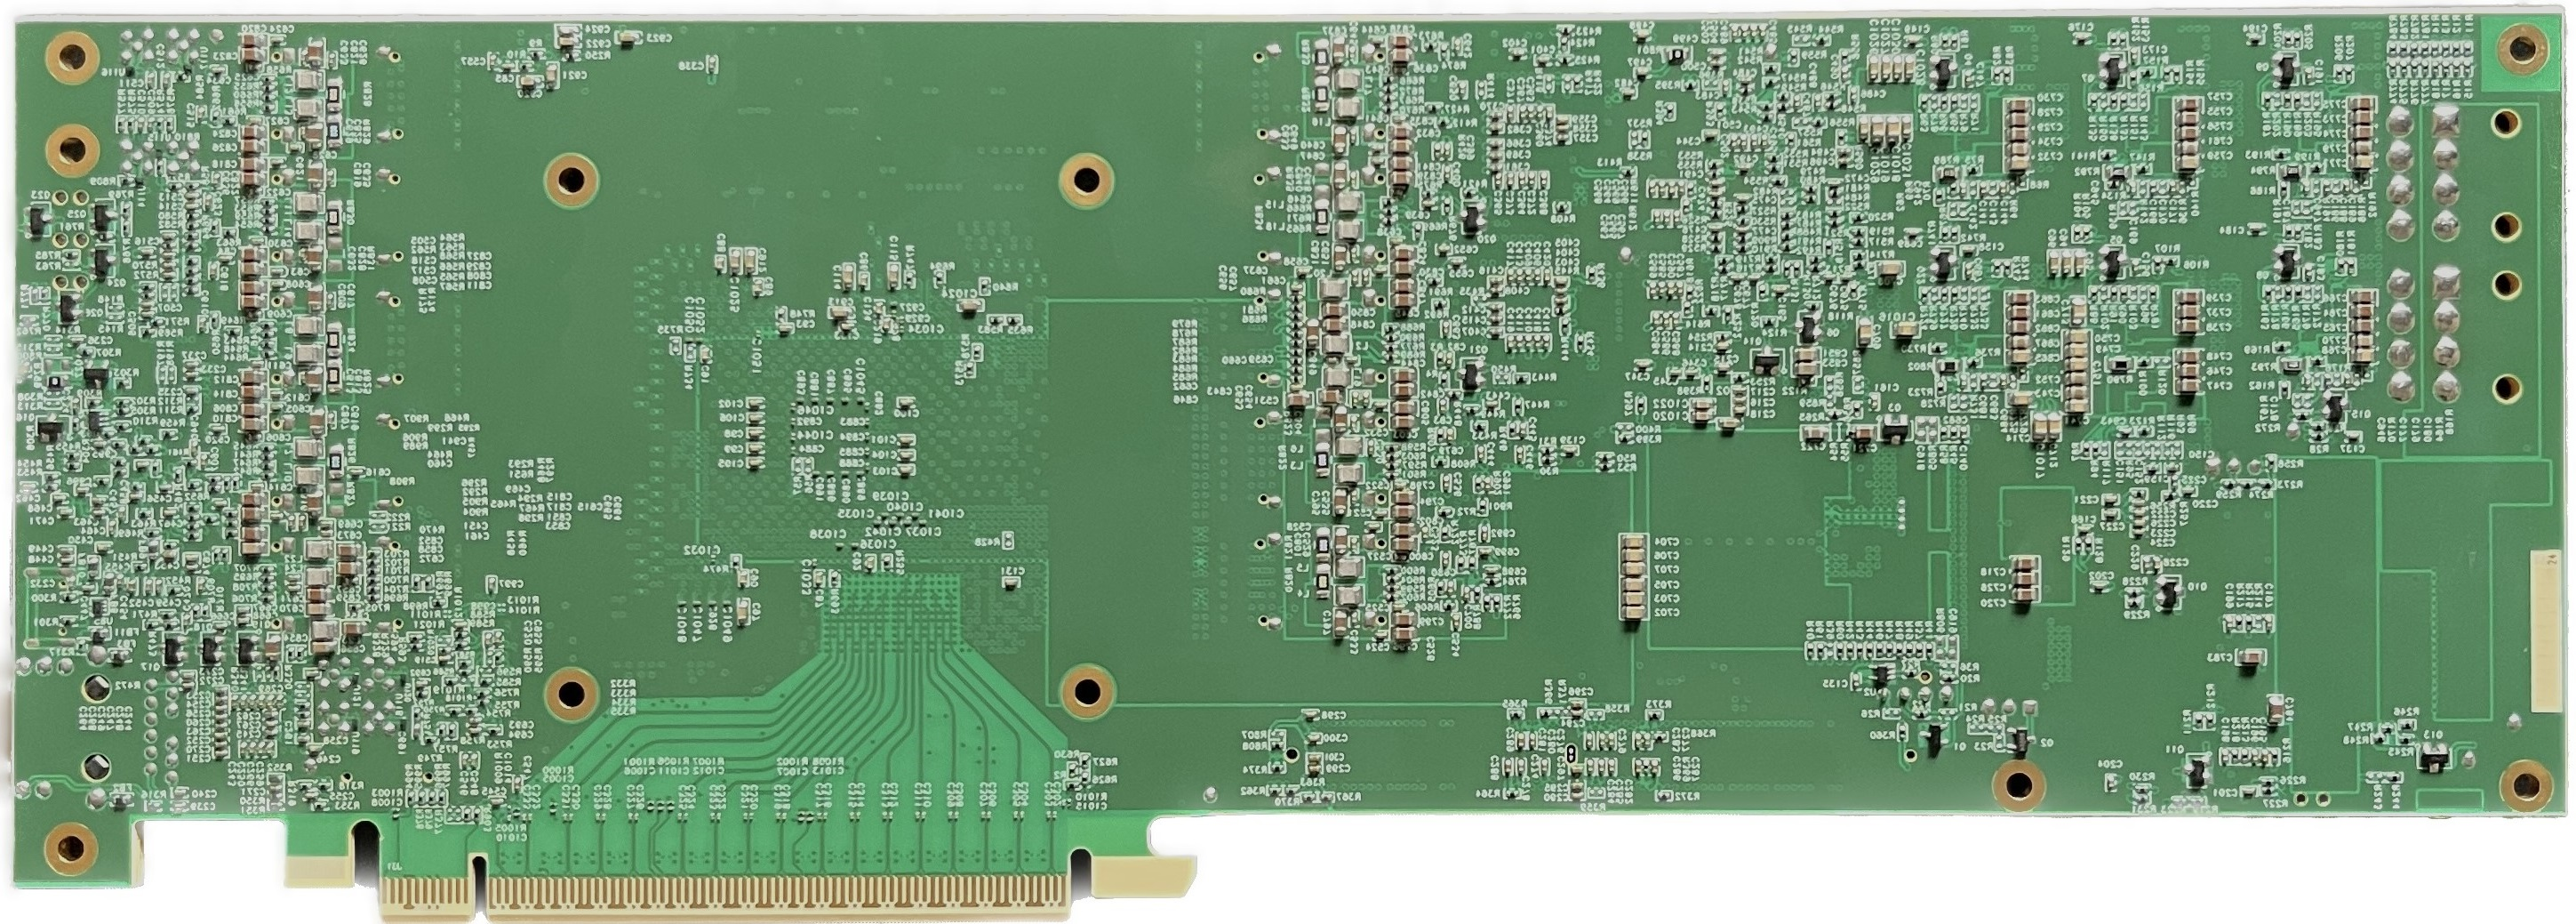
\includegraphics[width=\textwidth]{images/felix/flx155_bot.jpg}
    \caption{FLX-155 rear view.}
    \label{fig:FLX-155-bot}
\end{subfigure}
\caption{FLX-155 hardware.}
\label{fig:FLX-155}
\end{figure}

\clearpage
\section{Firmware}
\label{sec:felix-firmware}

The \acs{FELIX} firmware handles physical layer connectivity, data buffering, and communication with the host through the \ac{PCIe} interface. There are different firmware "flavours" that are used depending on what \acl{FE} is using the \acs{FELIX} card.\\
Below is a comprehensive list of all the firmware types depending on the protocol the \acs{FELIX} card needs to communicate with.

\subsection{\acl{GBT} and Versatile Link}
\label{subsec:felix-gbt}

The \ac{GBT} chipset, combined with the Versatile Link optical technology \cite{gbt-versatile-link}, have evolved from \ac{CERN}'s Radiation Hard Optical Link Project. Versatile Link is a radiation-tolerant bi-directional optical link for data transfer among \acs{GBT} endpoints. The \ac{GBT} protocol aggregates lower-bandwidth logical links (\acs{E-link}s) from front-end devices into a single link operating at up to 5~Gb/s.

\begin{definition}
\label{def:elink}
An \acs{E-link} is a virtual lane inside a physical optical link. By using multiple \acs{E-link}s, it is possible to transmit multiple data streams in parallel.
\end{definition}

\begin{figure}[H]
\centering
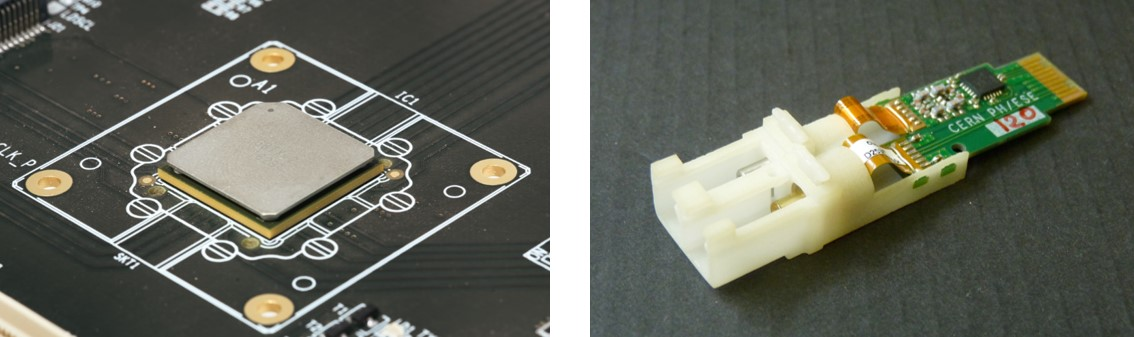
\includegraphics[width=\textwidth]{images/felix/gbt.jpg}
\caption[GBT and Versatile Link]{\acs{GBT} chip (left) and Versatile Link (right). Source \protect\cite{gbt-versatile-link}}
\label{fig:gbt-versalink-combined}
\end{figure}

\subsection{\acf{lpGBT}}
\label{subsec:felix-lpgbt}

The \acf{lpGBT} \cite{lpgbt} is an evolution of the \acf{GBT} project and is a radiation tolerant \acs{ASIC} that can be used to implement multipurpose high speed bidirectional optical links for high-energy physics experiment, with 2.56~Gb/s downlinks (readout to front-end) and 5.12~Gb/s or 10.24~Gb/s uplinks (front-end to readout), depending on the selected operation mode. The aim of \acs{lpGBT} is to allow a single bidirectional link to be used simultaneously for data readout, trigger data, timing, experiment control and monitoring.

\begin{figure}[H]
\centering
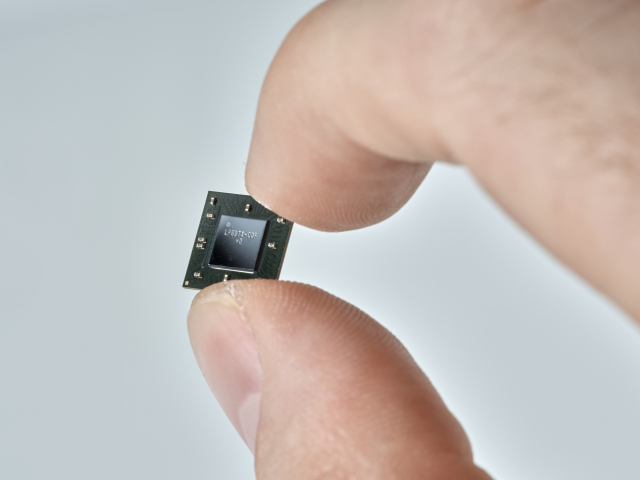
\includegraphics[width=\textwidth]{images/felix/lpgbt.jpg}
\caption[lpGBT chip]{\acs{lpGBT} chip. Source \protect\cite{lpgbt-image-source}}
\label{fig:lpgbt}
\end{figure}

\subsection{FULL Mode}
\label{subsec:felix-fullmode}

The FULL mode protocol \cite{fullmode} is used for \acl{FE} electronics with no radiation constraints, and it requires less \acs{FPGA} resources compared to \acs{GBT}. FULL mode provides a single, wide data stream without using the \acs{E-link} substructures or the handshaking mechanisms in \acs{GBT}/\acs{lpGBT}, and allows a data rate of 9.6~Gb/s. After 8b/10b encoding, this yields a peak uplink payload of 7.68~Gb/s.\\
Downstream traffic at 9.6~Gb/s transmits timing signals (such as the 40.079~MHz \acs{LHC} clock) and control data from the \acf{LTI}.\\
Early releases of FULL mode reused GBT-compatible downlinks for legacy \acf{TTC} messaging.

\subsection{Interlaken Mode}
\label{subsec:felix-interlaken}

For even higher throughput, the firmware supports the Interlaken protocol \cite{InterlakenSpec} with link speeds as high as 25~Gb/s. Interlaken follows a structure similar to FULL mode, offering a single high-speed data channel without sub-channels. Downstream communication relies on a 9.6~Gb/s link and conveys \acs{LTI} messages equivalently to FULL mode.

\subsection{\acs{ATLAS} \acs{ITk} Pixel and Strip Compatibility}
\label{subsec:felix-itk}

\acf{ITk} \cite{atlas-itk-pixel-detector} is a new detector meant for Phase II \acs{ATLAS}.
A dedicated firmware has been developed to interface with  Pixel and Strip sub-detectors.\\

The \emph{Strip} flavour was designed to read out the \acs{ITk} Strip detector over \acs{lpGBT} with 8b/10b e-links.\\
The \emph{Pixel} flavour was designed to read out the \acs{ITk} Pixel detector over \acs{lpGBT} with Aurora \cite{aurora-protocol} e-links.\\

Aurora \cite{aurora-protocol} is a high-speed, link layer, serial communication protocol developed by Xilinx, which is used to transmit data between the \acs{FPGA} and the front-end electronics.

\section{Software}

All the software for the \acs{FELIX} project is open source and hosted on Gitlab under the name of felix-distribution \cite{felix-distribution}. This software is formally supported and built for systems using the AlmaLinux 9 \acl{OS}.

\subsection{\acs{FELIX} drivers}

\subsubsection{flx\_driver}

The \texttt{flx} driver~\cite{felix-driver} is a device driver developed for Linux for \acs{PCIe}-based hardware. It is responsible for detecting \acs{FELIX} cards, managing hardware interrupts, and exposing a set of \texttt{ioctl} interfaces for user-space interaction. Within the \acs{ATLAS} software framework, the \texttt{flx} driver is typically deployed in conjunction with the \texttt{cmem\_rcc} driver, and optionally, the \texttt{io\_rcc} driver, to provide support for cross-device communication and memory management.

\subsubsection{cmem\_rcc}

The allocation of contiguous memory buffers is a requirement for high-performance \acf{DMA} operations in general, and for data acquisition systems such as \acs{FELIX} in particular. In 2018, the standard \ac{CMA} was evaluated and found inadequate for \ac{FELIX} requirements, primarily due to limitations in support and documentation \cite{cmem-rcc}.

The cmem\_rcc \cite{cmem-rcc} package, well established within the \acs{ATLAS} experiment, was selected as the baseline solution. The cmem\_rcc driver and its associated user-space library is based on the kernel's \texttt{alloc\_pages\_node()} and \texttt{alloc\_pages()} system calls. These calls allow memory to be allocated either from a specific \ac{NUMA} node or without \ac{NUMA} awareness, providing flexibility for deployment on multi-socket systems.

cmem\_rcc supports two allocation strategies: (1) on-demand allocation of individual buffers, and (2) pre-allocation of a large contiguous memory region at driver load time, from which user applications can request fragments as needed.

The driver supports concurrency and synchronization, using spinlocks to ensure thread safety on \ac{SMP} systems \cite{cmem-rcc}.

\subsection{Felix Distribution}

Felix Distribution \cite{felix-distribution} is a repository in which all the \acs{FELIX}-related software is contained. As a logical consequence, \acs{FELIX} software is a collection of projects that are separately developed.\\
Below is a non-comprehensive list of components of Felix Distribution --- followed by a brief description --- focusing only on modules relevant to the thesis.

\textbf{elinkconfig}\\
The \texttt{elinkconfig} module is responsible for the configuration and management of \acs{E-link}s. This module provides utilities to enable and disable \acs{E-link}s define, modify, and query the settings of each \acs{E-link}.

\textbf{felix-bus-fs}\\
\texttt{felix-bus} translates \acs{FELIX} specific IDs (see Definition~\ref{def:FID}) into generic network information by exposing the information as files within the Linux file system. In the next chapter there will be a more detailed explanation of what \texttt{felix-bus} does (see Section~\ref{sec:felix_bus}).

\textbf{felix-star}\\
\texttt{felix-star} is the primary readout application. More on this module in the next chapter \emph{felix-star} (Chapter~\ref{chap:felix_star}).

\textbf{felix-client}\\
\texttt{felix-client} is the client application that \acs{FELIX} software users (like for example the Detector software developers) use to communicate with server applications of \texttt{felix-star}.

\textbf{felix-monitor}\\
The \texttt{felix-monitor} module is responsible for monitoring the status and performance of the \acs{FELIX} system. It collects and reports \acs{FELIX}-specific metrics, as well as more general ones like data throughput and error rates.

\textbf{flxcard}\\
The \texttt{flxcard} module is the user-space driver library of a \acs{FELIX card}, and serves as the primary hardware abstraction layer for the \acs{FELIX} \acs{PCIe} cards installed in the host system.

\textbf{ftools}\\
The \texttt{ftools} module comprises a suite of utility programs and scripts designed to perform common --- and often low-level --- tasks in the \acs{FELIX} environment, generally used for testing and debugging \acs{FELIX} dataflow and control operations including interaction with remote peers.

\textbf{netio3}\\
\texttt{netio3} will be expanded upon in the next chapter \emph{Netio3} (Chapter~\ref{chap:netio3}).

\clearpage
\section{Personal Contributions - Hardware Testing and Assembly}
\label{sec:felix-hardware-contributions}

The primary hardware contribution involved the testing (Figures~\ref{fig:felix-testing}, \ref{fig:bist}, \ref{fig:eyescan-test}) and assembly (Figure~\ref{fig:batch-felix-cards}) of the FLX-182-1B cards. I subjected the cards to a series of previously defined tests:

\begin{enumerate}
    \item \textbf{Component Verification}
    \begin{itemize}
        \item Visually inspected the most important discrete components (e.g. resistors, capacitors)
        \item Measured those components using a multimeter
    \end{itemize}

    \item \textbf{Power Management Configuration}
    \begin{itemize}
        \item Programmed the power delivery controller (ADM1266)
    \end{itemize}

    \item \textbf{FPGA Programming}
    \begin{itemize}
        \item Uploaded the programmable logic test firmware onto the FPGA and flash memory
    \end{itemize}

    \item \textbf{Mechanical Assembly}
    \begin{itemize}
        \item Assembled the fansink, \acs{PCIe} bracket, DDR module, and FireFly modules
        \item Installed a jumper on J40 (adjacent to fan power connector), connecting the top pin (GND) with the central pin. This sets the fan at maximum speed upon power-on
    \end{itemize}

    \item \textbf{FPGA Functionality Test}
    \begin{itemize}
        \item Prepared an SD card containing both the boot loader and the PetaLinux/BIST firmware
        \item Completed electrical and optical verification steps
    \end{itemize}

    \item \textbf{Front Panel Electrical Signals Test}
    \begin{itemize}
        \item Validated all front-panel electrical connections
    \end{itemize}
\end{enumerate}

\begin{figure}[H]
\centering
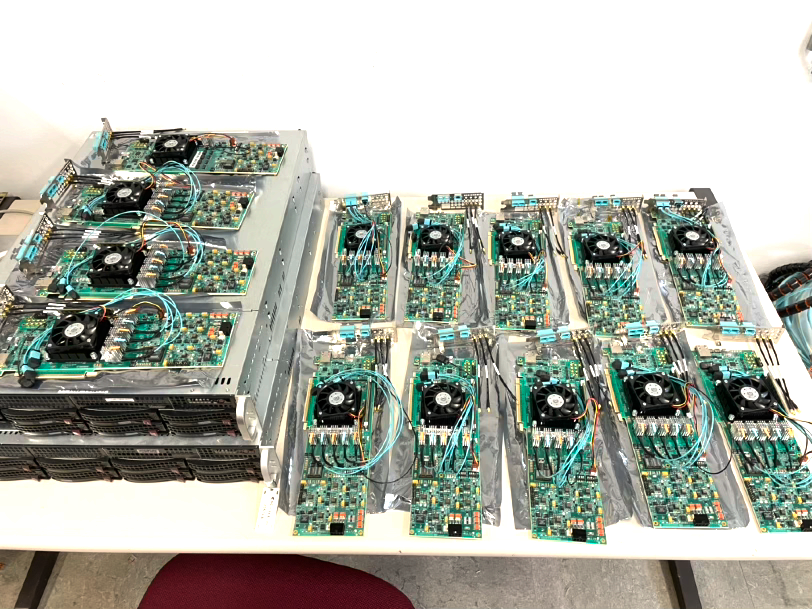
\includegraphics[width=\textwidth]{images/contributions/felix-cards.png}
\caption{A batch of fully tested and assembled FLX-182-1B cards.}
\label{fig:batch-felix-cards}
\end{figure}

\subsubsection{Tools}

The assembly of the cards required specialized equipment, and programming the power delivery controller was performed using an Aardvark I2C/SPI host adapter. The \acs{FPGA} was configured with Vivado \cite{vivado}. Electrical signal verification and validation of the front panel and active components involved the use of an oscilloscope, a power supply unit, and a function generator. Additionally, a server running with a \acs{DHCP} server was utilized to test the fiber connections, and a \acs{PCIe} loopback test card was employed to ensure proper \acs{PCIe} functionality.

\clearpage
\begin{figure}[htbp]
\begin{minipage}{0.9\textwidth}
\centering
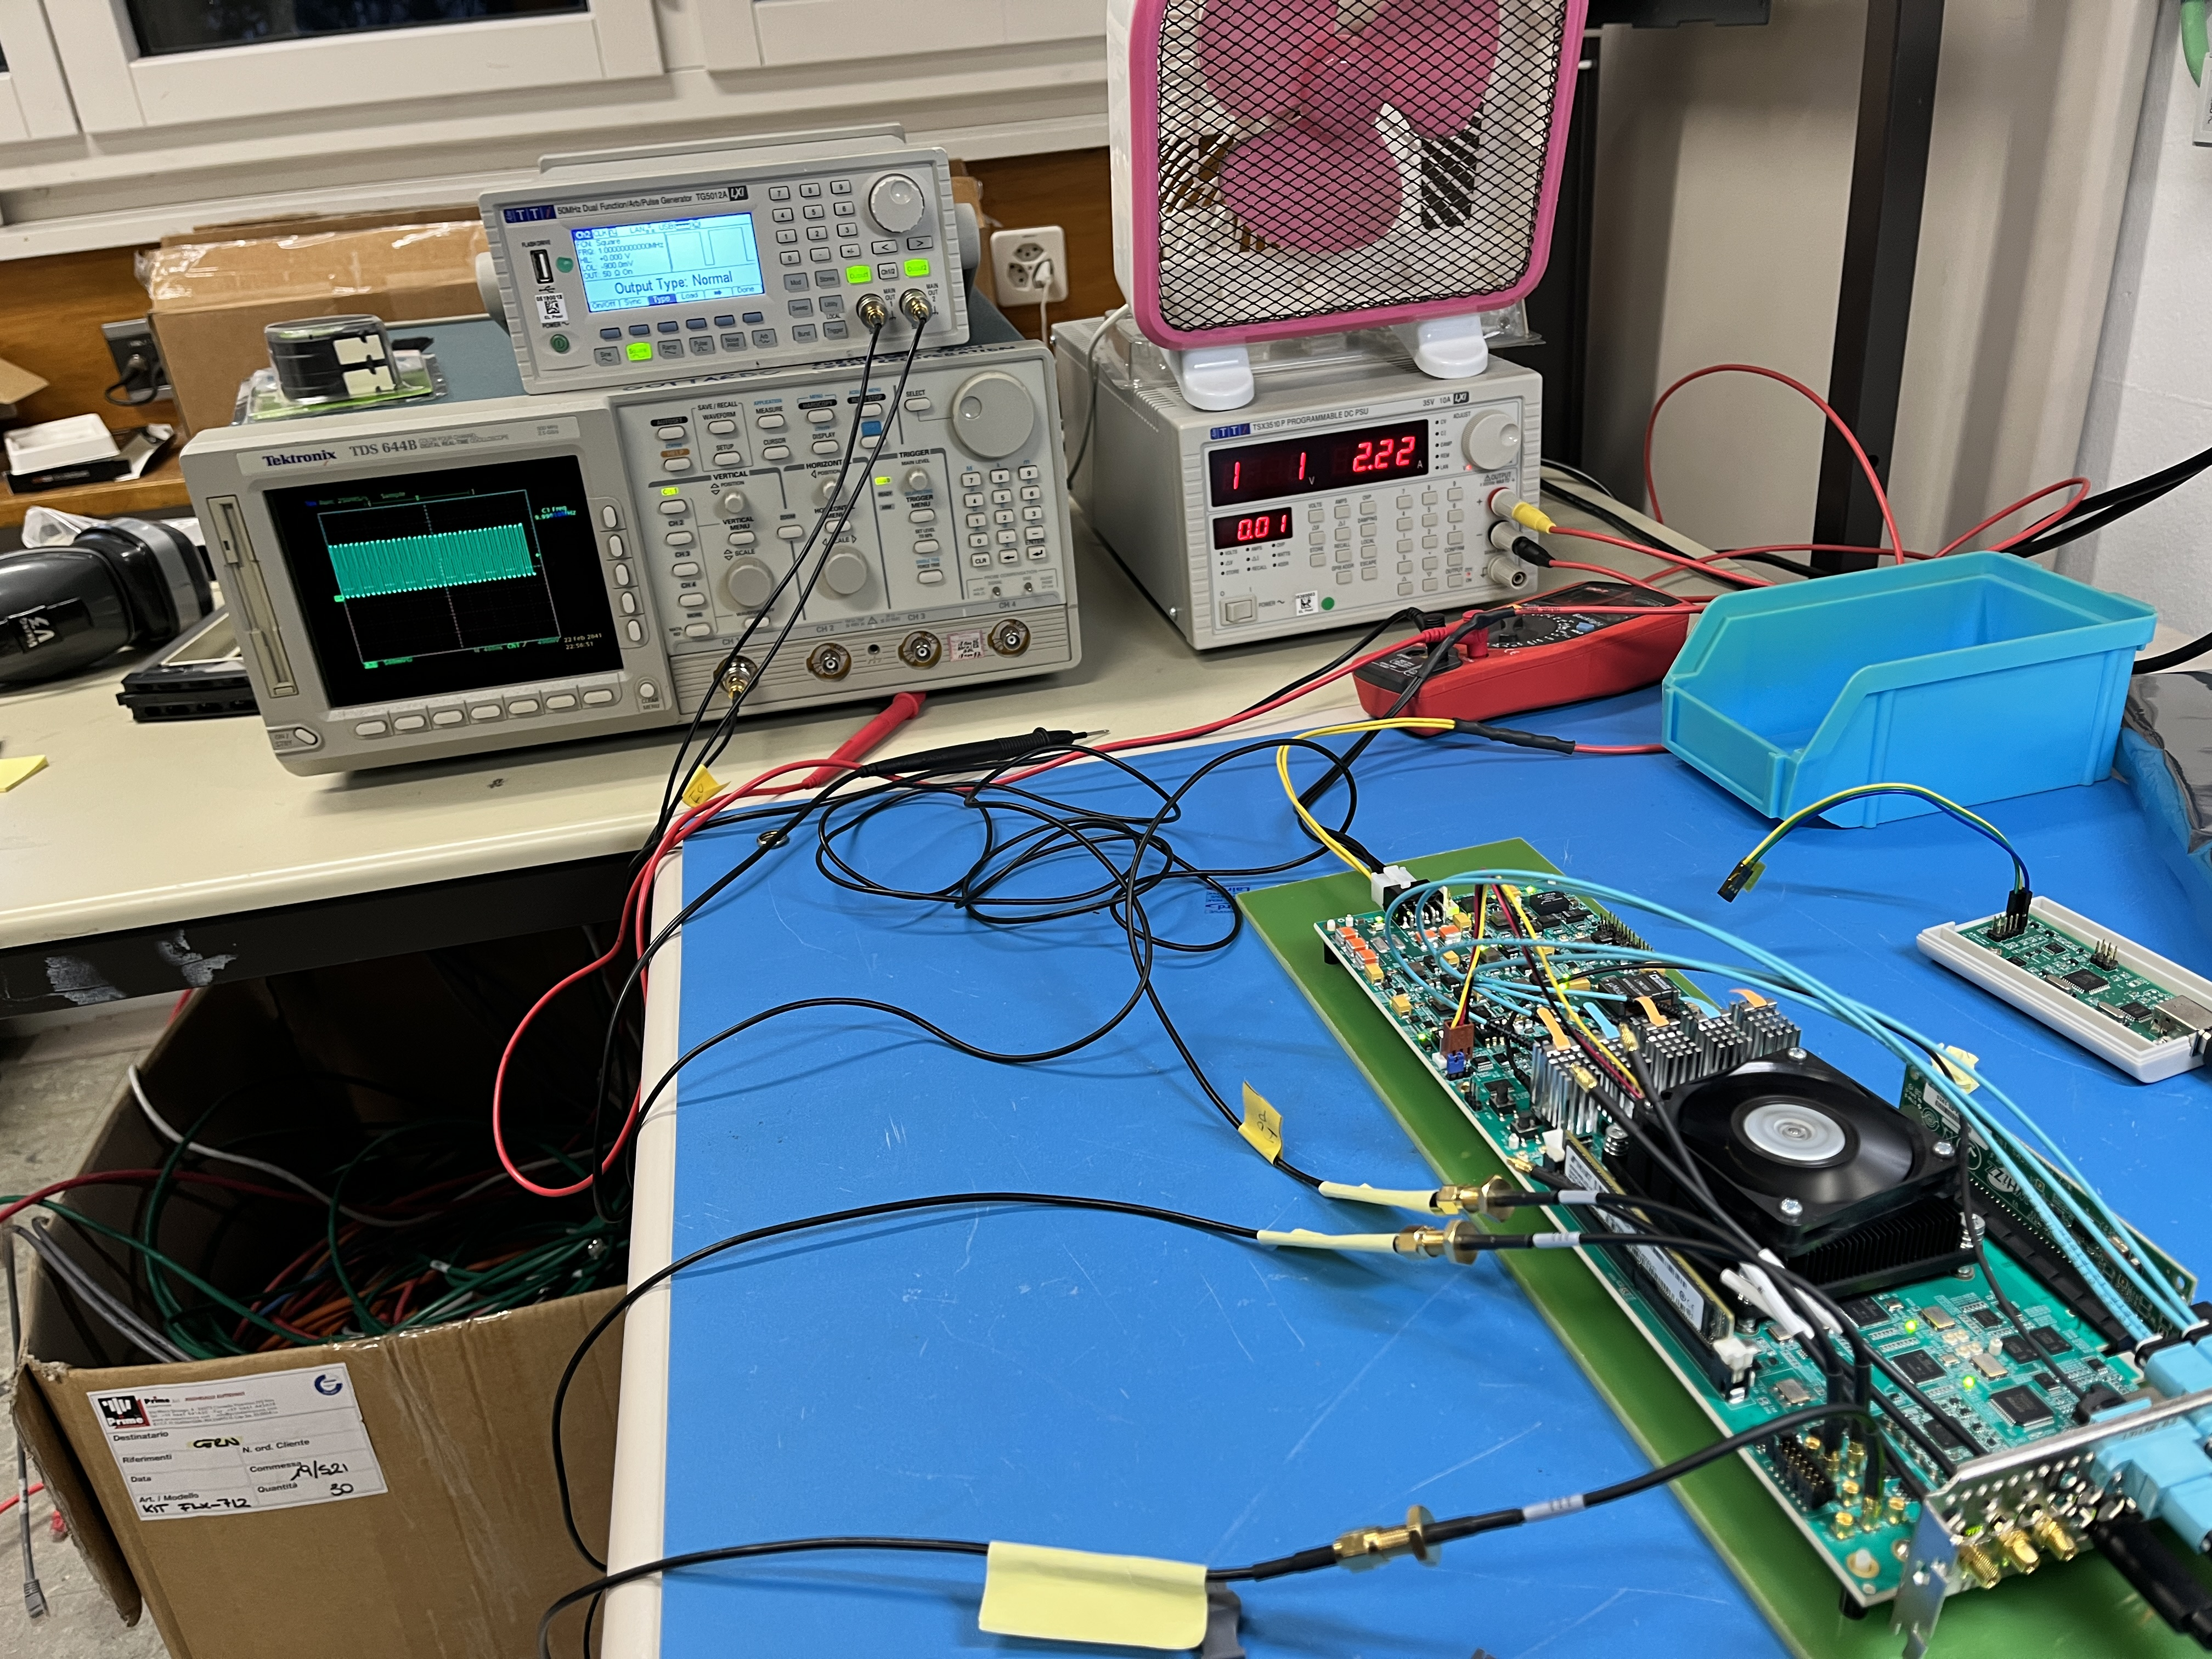
\includegraphics[width=0.8\textwidth]{images/contributions/felix-card-testing.jpg}
\caption[FELIX card testing setup]{Testing a \acs{FELIX} card. The PSU on the right, with a fan on top to help cool the \acs{FPGA}. Also on the right detached the Aardvark host adapter. The function generator is on top of the oscilloscope, with the probes attached to the electrical triggers. The \acs{PCIe} loopback scan is barely visible behind the aquamarine-colored fiber-optic cables, just on top of the mounted fan. What is not visible is the fibers connecting in a loopback the Firefly \protect\cite{firefly-optical-transceiver} optical transceiver modules, the \acs{JTAG} and UART cables.}
\label{fig:felix-testing}
\end{minipage}\hfill
\begin{minipage}{0.9\textwidth}
\centering
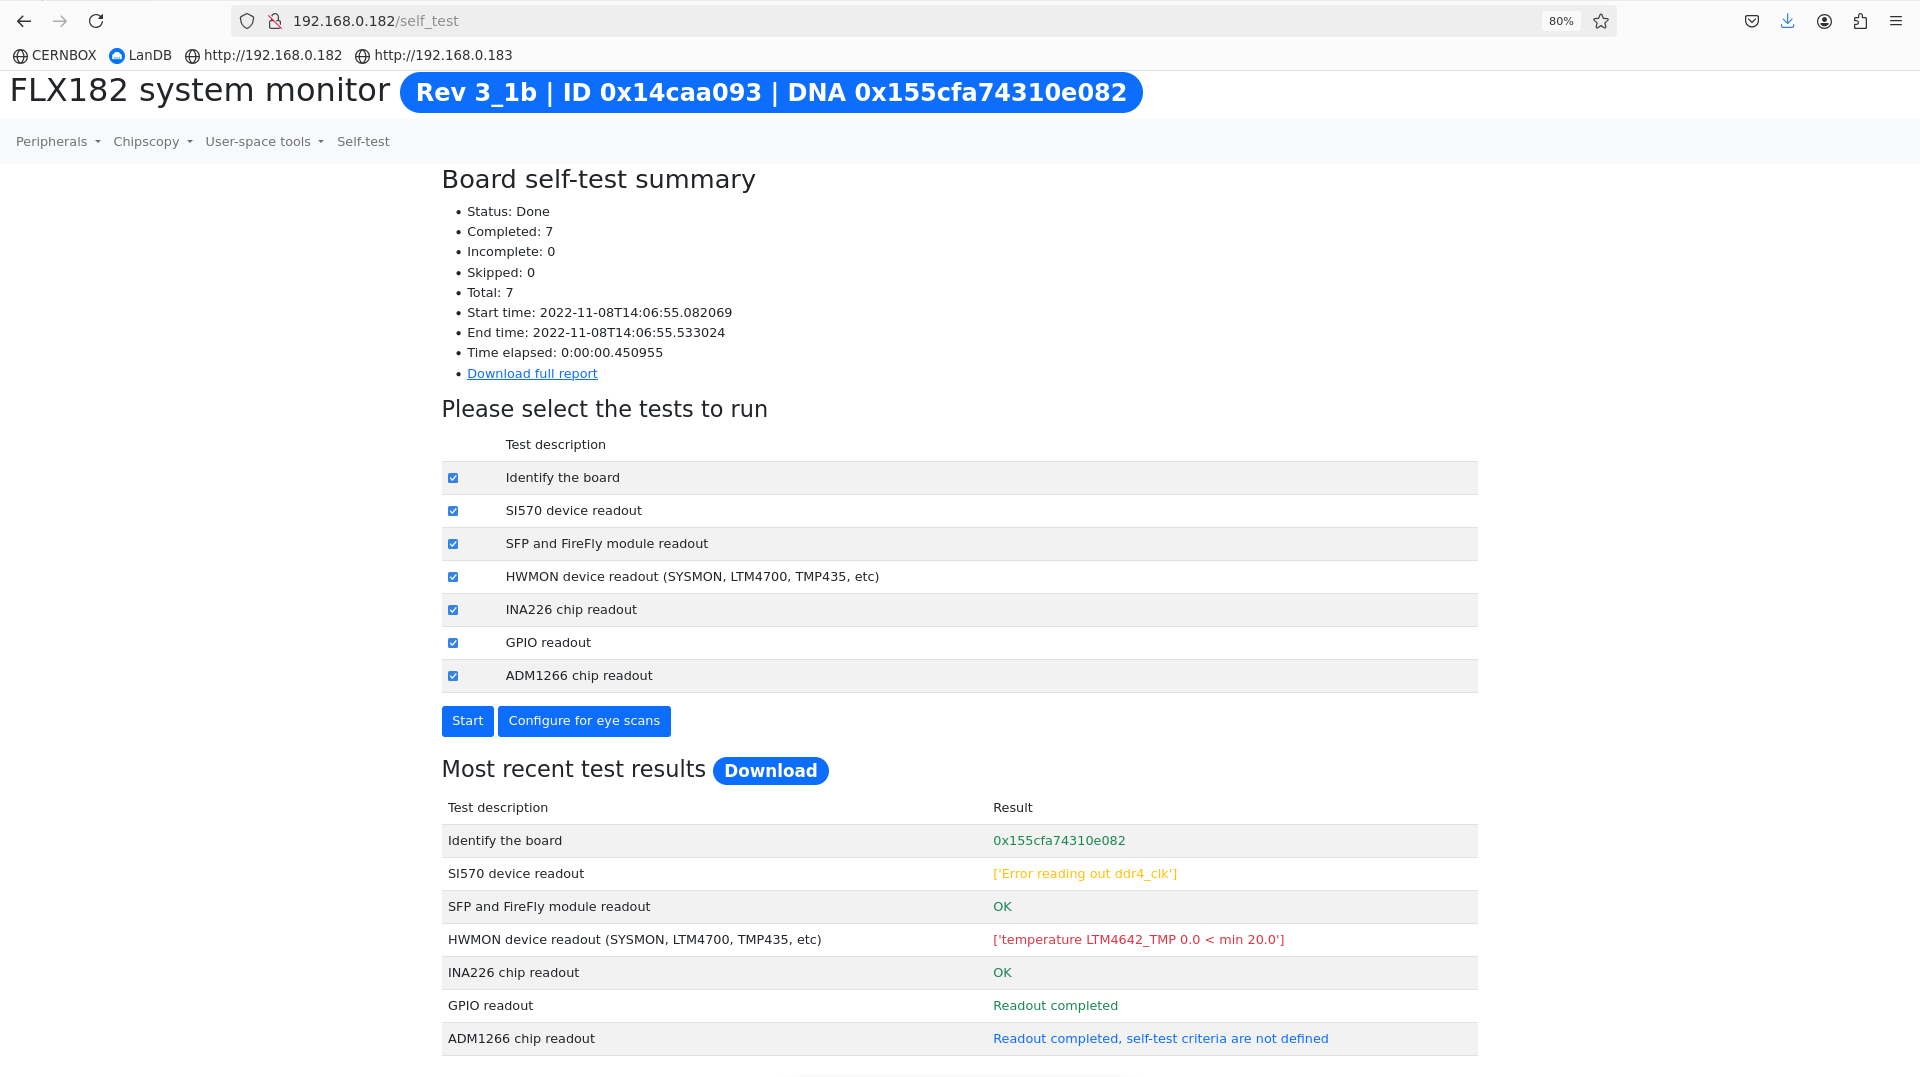
\includegraphics[width=\textwidth]{images/contributions/BIST.png}
\caption[Builtin Selftest screenshot]{Builtin Selftest. The \acs{DHCP} server is needed to give an IP to the card; an Ethernet cable connects the card to the server. The \acs{FELIX} card exposes this website which allows to check if all the active components in the \acs{PCB} are reachable and prepares the card for the eyescan test.}
\label{fig:bist}
\end{minipage}
\end{figure}

\begin{figure}[H]
\centering
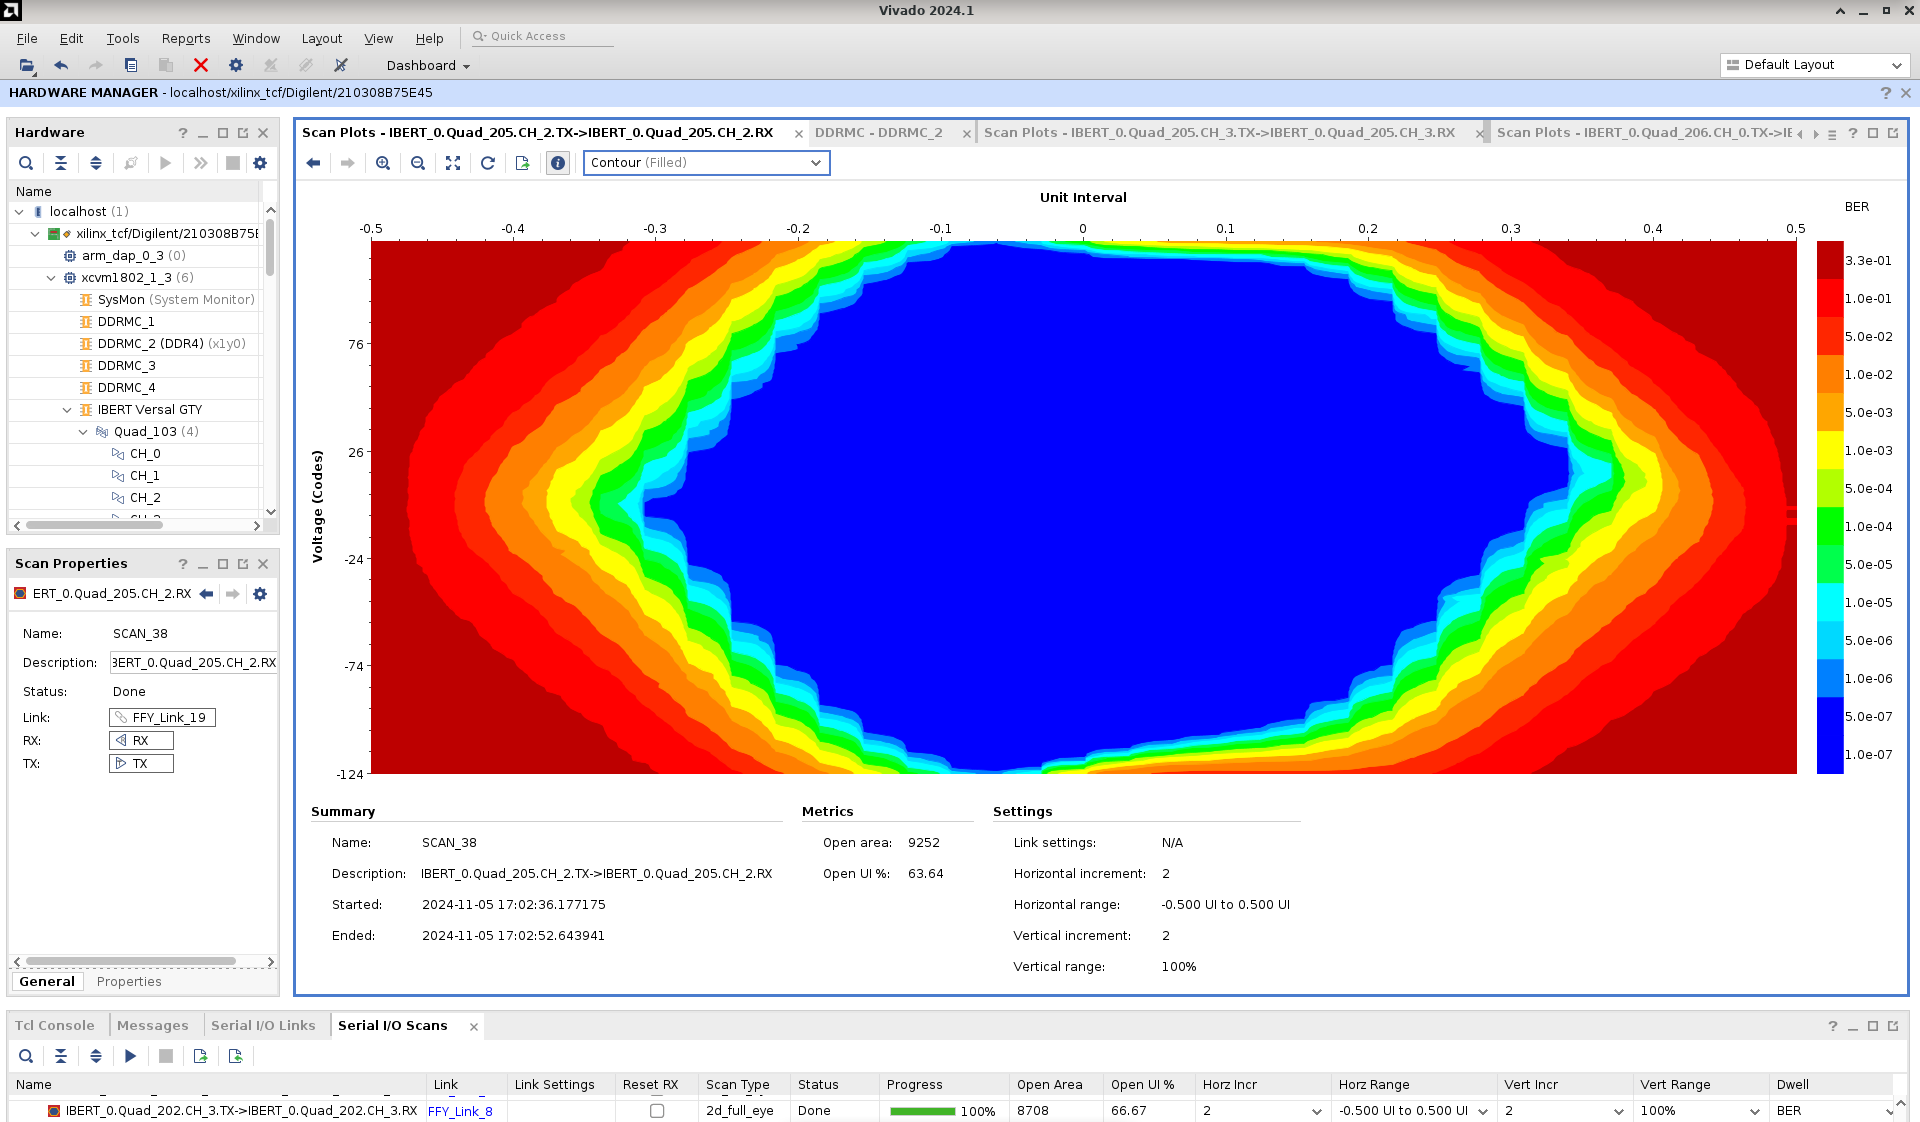
\includegraphics[width=\textwidth]{images/contributions/eyescan.png}
\caption[Sample of the eyescan of a GTY transceiver]{Sample of the eyescan of a GTY transceiver. Those transceivers receive the signals from the Firefly \protect\cite{firefly-optical-transceiver} modules and make them available to the FPGA. The GTY transceivers live inside the FPGA produced by AMD. This image represents the error rate of one transceiver. The blue part indicates a low error rate, while red indicates a high error rate\\
Y axis: the voltage received by the transceiver\\
X axis: Unit Intervals fractions, which essentially means that the signal is brought out of phase by a percentage of one clock cycle. A unit interval corresponds to a clock period.}
\label{fig:eyescan-test}
\end{figure}

\clearpage
\subsubsection{Challenges}

There is an official table listing the most critical discrete components on the \ac{PCB}; an excerpt is provided below in Table~\ref{tab:pcb-rail-measurements} (without excessive detail):

\begin{table}[H]
\centering
\caption[Reference value of resistors]{Key power rail sensor resistors and feedback impedance measurements for FLX-182-1B.}
\label{tab:pcb-rail-measurements}
\resizebox{\linewidth}{!}{%
\begin{tabular}{|l|l|l|l|l|}
\hline
\textbf{Module} & \textbf{RefDes} & \textbf{Power Rail} & \textbf{Sensor Resistor (Ohm)} & \textbf{Reference (Ohm)} \\
\hline
LTM4700 & U1  & VCCINT   & R884 1.0    & 1.0 \\
LTM4638 & U7  & MGTAVCC  & R940 12.2   & 12.2 \\
LTM4638 & U3  & MGTAVTT  & R934 278.2  & 278.2 \\
LTM4638 & U2  & SYS12    & R933 87.6   & 87.6 \\
LTM4638 & U4  & SYS15    & R935 194.9  & 194.9 \\
LTM4638 & U6  & SYS18    & R939 270.6  & 270.6 \\
LTM4638 & U5  & SYS33    & R936 101.9  & 101.9 \\
LTM4642 & U84 & SYS25    & R938 5.89k  & 5.89k \\
\hline
\end{tabular}%
}
\end{table}

\vspace{1em}

\begin{table}[ht]
\centering
\resizebox{\linewidth}{!}{%
\begin{tabular}{|l|l|l|l|}
\hline
\textbf{Power Rail} & \textbf{FB Impedance RefDes} & \textbf{Measured Impedance} & \textbf{Notes} \\
\hline
SYS38        & R937  & $\sim$300k    & Jumper resistors present \\
MGTVCCAUX    & R928  & 4.836k        & ADP124 U35 \\
DDR4 VTT     & R795  & 4.102k        & TPS51200 U58 \\
VCC5V        & R929  & 6.26k         & TPSM5601R5 U52 \\
VCC5VM       & R930  & 125.6         & U74 \\
\hline
\end{tabular}%
}
\caption{Power rail impedance measurements.}
\label{tab:impedance}
\end{table}

Due to the high density of components and their sizes, precisely locating them was challenging, and doing so consistently across different cards and production batches proved difficult. Furthermore, not all components needed the same type of inspection. Some discrete components required just visual inspection while other required one or more measurements. To help with the task, I developed a visual aid (Figure~\ref{fig:FLX-182-hardware-inspection} and ) to translate the tables into an image, thus streamlining the inspection process. Components were color-coded according to the type of inspection required.

\begin{figure}[H]
\centering
\begin{subfigure}[b]{\textwidth}
    \centering
    \includegraphics[width=\textwidth]{images/contributions/Resistors_front.jpg}
    \caption{Top view: FLX-182-1B color coded components to inspect.}
    \label{fig:FLX-182-top-resistors}
\end{subfigure}

\vspace{0.2cm}

\begin{subfigure}[b]{\textwidth}
    \centering
    \includegraphics[width=\textwidth]{images/contributions/Resistors_back.jpg}
    \caption{Bottom view: FLX-182-1B color coded components to inspect.}
    \label{fig:FLX-182-bot-resistors}
\end{subfigure}
\caption{FLX-182-1B hardware probing aid.}
\label{fig:FLX-182-hardware-inspection}
\end{figure}

A significant challenge involved isolating faults in malfunctioning cards. In two instances there was a blown capacitor, making those cases the easiest to diagnose. One notable issue arose with cards that failed to boot from the SD card, which was traced to a defect in the SD interface adapter.

Upon diagnosing the issues, I prepared detailed documentation to guide technicians in repairing the affected cards and replacing the faulty components.

Not all problem diagnosis was conducted independently; I collaborated with hardware engineers at \acf{BNL}.

\chapter{felix-star}
\label{chap:felix_star}

\texttt{felix-star} \cite{felix-software-specs} is the primary data routing software of felix-distribution. It is responsible for transfering data both within the \acs{FELIX} host and between network peers. To clarify, the name originates from \ac{STAR}, but since it is now multithreaded, "star" will be referred purely as a name.

\texttt{felix-star} does not refer to a single application, instead, it represents a suite of independent applications built on a common architecture. Each application has a well-defined functionality. This design keeps the codebase simpler to maintain, makes issues easier to localize, and allows individual components to be independently restarted without affecting the overall system.

All \texttt{felix-star} applications are managed by an orchestrator application. At the moment such application is \texttt{supervisord} \cite{supervisord}— which also is under consideration for Phase-II.\\
\texttt{Supervisor} \cite{supervisord} is a client/server system that allows its users to monitor and control a number of processes on UNIX-like operating systems. \texttt{supervisord} is the server part of Supervisor and it is responsible for starting child programs, responding to commands from clients, restarting crashed or exited subprocesseses, logging its subprocess stdout and stderr output, and generating and handling “events” corresponding to points in subprocess lifetimes.

The to-host direction in \texttt{felix-star} refers to data processed and sent from the \acs{FELIX} card to client applications, according to link subscriptions (uplink direction). In the from-host (or to-flx) direction, messages that are destined to enabled links are sent to the \acs{FELIX} card, which routes them to the front-end hardware (downlink direction). felix-bus (Section~\ref{sec:felix_bus}) advertises active links managed by a \acs{FELIX} host, so that client applications can look them up and know what addresses are available to receive and send data.

Communication between \texttt{felix-star} processes and network peers is handled by the \texttt{netio3} library.\\
 Two communication modes are supported:

\begin{itemize}
    \item \textbf{Buffered mode:} Coalesces many small messages (e.g., tens of bytes) into larger buffers called netio pages. When the page occupancy crosses a certain threshold, the buffer is sent. This mode reduces transfer overhead.
    \item \textbf{Unbuffered mode:} Suited for high-throughput scenarios involving large messages (in the kilobyte range). The unbuffered mode enables zero-copy sending that avoids what are necessary copies for the buffered mode.
\end{itemize}

Client applications (e.g., the Software ROD/Data Handler \cite{swrod-repository} or \acs{OPC-UA} \cite{opc-ua} server) do not interface directly with \texttt{netio3}. Instead, they use the \texttt{felix-client-thread} \acs{API}, which simplifies connection setup by automatically reading parameters (e.g., mode, page size/count) from felix-bus and hiding the lookup mechanism. Another feature of \texttt{felix-client-thread} is to offer a synchronous layer around the asynchronous network library.

\texttt{felix-star} can produce JSON-formatted monitoring data and write it to the monitoring system of choice. External monitoring tools can read this data. In the latest releases a web-based monitoring interface is available for a graphical lookup of the data (See section~\ref{sec:felix_monitoring}).

Below a visual aid that illustrates the \texttt{felix-star} software architecture (Figure~\ref{fig:felix-star})

\begin{figure}[htbp]
\centering
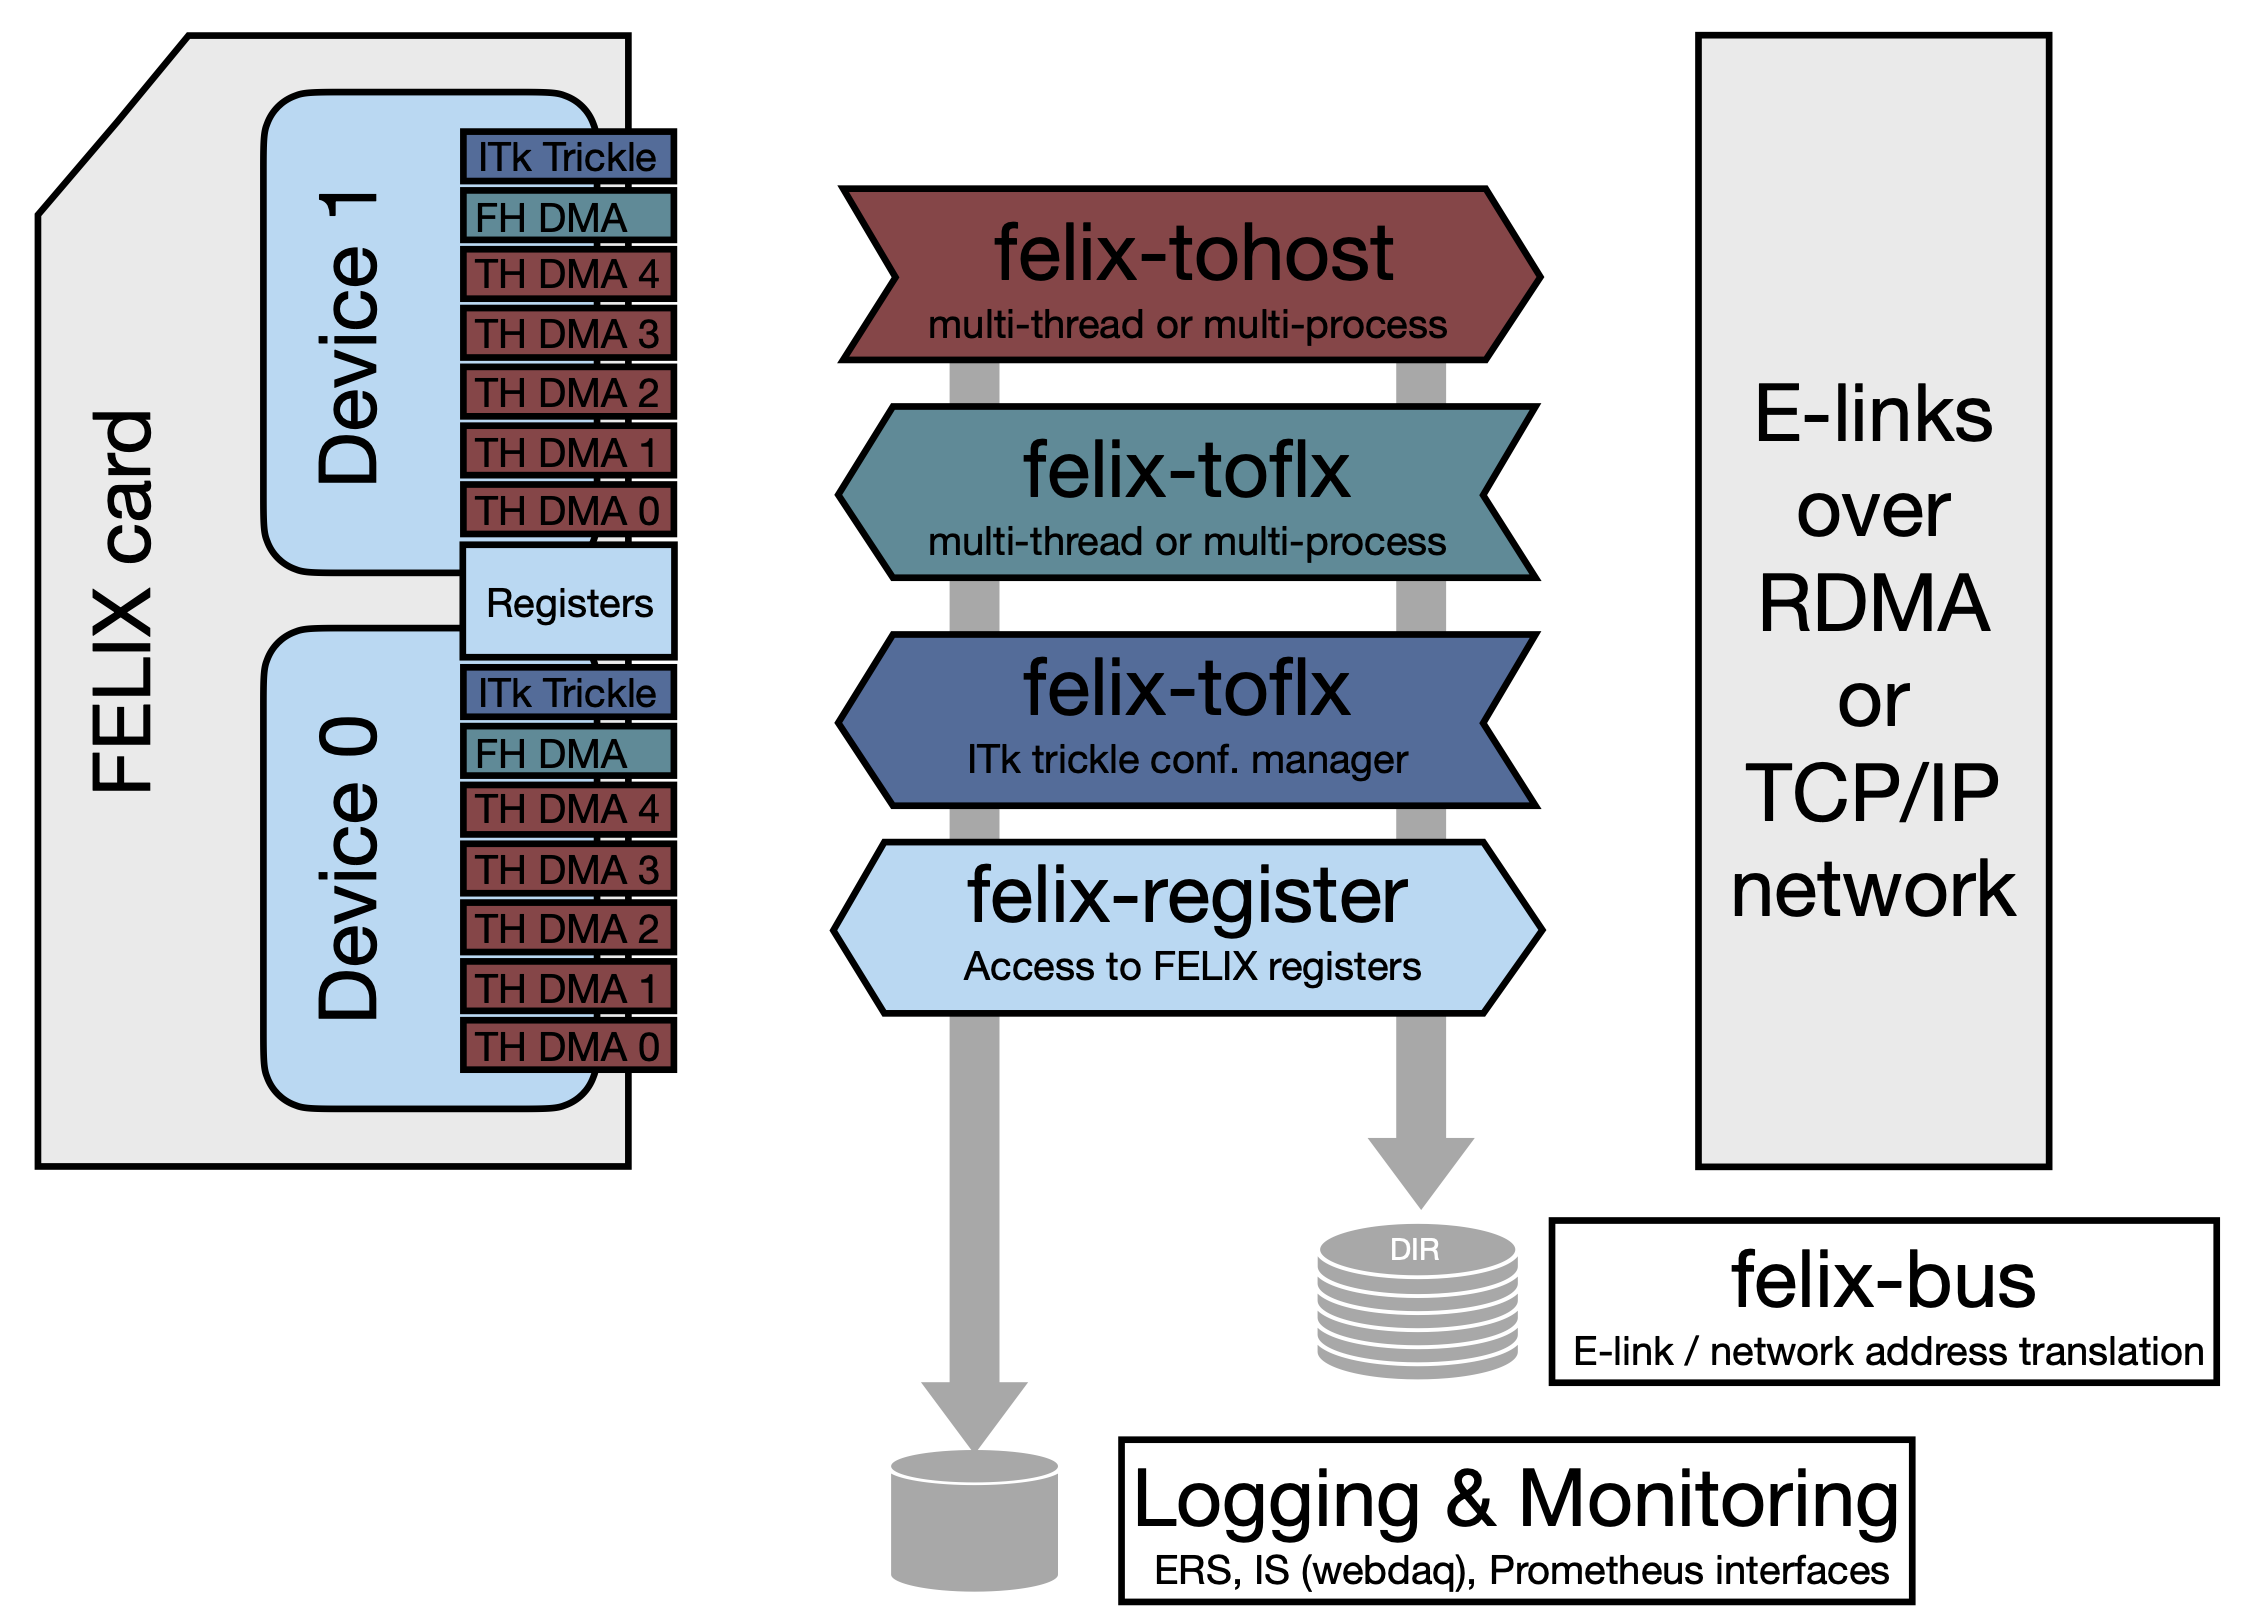
\includegraphics[width=0.8\textwidth]{images/felix/felix-star-architecture.png}
\caption[felix-star software architecture]{felix-star software architecture. The colours help understand what interacts with what. Briefly: felix-tohost reads from the same-coloured DMA buffers and sends the data over the network. felix-toflx does the opposite, takes data from the network and writes it into the DMA buffers. felix-register is used for RW operations on firmware registers. Image source \cite{felix-user-manual}}
\label{fig:felix-star}
\end{figure}

\clearpage
\section{FELIX-identifier}
\label{sec:felix_identifier}

\acs{E-link}s are identified by a 64-bit number called \ac{FID} \cite{fid}. Below is a definition of each field of the \acs{FID} followed by a visual representation.

\textbf{Version Identifier (VersionID):} The upper 4 bits of the FelixID, used to track revisions of the identifier format. Supports up to 16 versions, with 0x0 reserved for backward compatibility and 0x1 as the current version.

\textbf{Detector Identifier (DetectorID):} An 8-bit field that identifies the detector system. Allows for up to 255 detectors, aligning with the ATLAS Event Format.

\textbf{Connector Identifier (ConnectorID):} A 16-bit field that identifies fibre trunks (physical input units). Supports up to 65,536 connectors per detector, providing flexibility for future expansions.

\textbf{Link Identifier (LinkID):} A 14-bit field that distinguishes optical links within a fibre trunk. The highest bit is reserved for virtual links, leaving 13 bits for physical links, supporting up to 16,384 identifiers.

\textbf{Transport Identifier (TransportID):} A 14-bit field that subdivides links into logical E-links (for GBT mode) or indicates protocol and direction. Includes 6 bits for GBT E-Link ID, 1 bit for direction, and 7 bits for protocol, supporting up to 127 protocols.

\textbf{Stream Identifier (StreamID):} An 8-bit field that denotes specific streams within a link. Supports up to 255 streams per E-link or FULL mode link.


\begin{definition}
\label{def:FID}
\acs{FELIX}-identifier:

\begin{table}[htbp]
\centering
\caption[FELIX Identifier Fields - 64 bits]{FELIX Identifier Fields - 64 bits.\label{lst:felix_identifier}}
\begin{tabular}{|c|c|c|c|c|c|}
\hline
4 bits & 8 bits & 16 bits & 14 bits & 14 bits & 8 bits \\ \hline
Version ID & Detector ID & Connector ID & Link ID & Transport ID & Stream ID \\ \hline
\end{tabular}
\end{table}

\end{definition}

\section{felix-bus}
\label{sec:felix_bus}

\texttt{felix-bus} is a hierarchical structure of JSON files that provides the mapping between active \acs{E-link}s and network addresses. This mapping is essentially a way to translate a detector-specific address into a more common network address. The directory containing felix-bus files must be accessible by all peers, this means that it should reside on a common network drive if communication occurs between different hosts.

A purpose of \texttt{felix-bus} is to minimize manual configuration of the \acs{FELIX} applications.
For example, client applications read from the felix-bus settings, like the number of network buffers and their size, and configure themselves accordingly.

The primary interface to felix-bus is \texttt{felix-client-thread}. It provides an \acs{API} for developing applications that can talk to \texttt{felix-star}. All references to “clients” in this context refer to applications using this \acs{API}.

\section{felix-tohost}

The application is responsible for reading data from \acs{DMA} transfer buffers, that live inside the contiguous memory allocated by \texttt{cmem\_rcc}, and send this data to the clients with a publish/subscribe pattern. Multiple such applications may run on a single host, each using a different DMA buffer. Each \acs{DMA} buffer is a circular buffer, with firmware and software monitoring and updating write and read pointers, respectively, to ensure that data is not overwritten.\\
The default behaviour is to spawn a single reader thread per \acs{DMA} buffer, but it is possible to configure the application to use multiple threads that can read each \acs{DMA} buffer.\\
\texttt{felix-tohost} supports both the physical hardware (felix-tohost) and a simulation of it (felix-tohost2file).

\subsection{felix-tohost data format}

Data packets arriving via the front-end links or virtual E-Links are referred to as “\texttt{chunks}” and can have an arbitrary size. Data inside the \acs{DMA} buffers is encoded in 1024-byte blocks. If a chunk is bigger than a block, or does not fit in the remaining space, it is divided in what is called a \texttt{subchunk}. Otherwise if a chunk does not completely fill a block, it is padded with zeroes and the whole block is sent after a timeout.\\
The reason for encoding data in \texttt{blocks} and not directly use \texttt{chunks} is because having \texttt{blocks} makes it easier for the software to handle the data: having a data format with a fixed size makes the memory alignment easier (constraint introduced by \acs{PCIe}), and similarly a fixed size makes \acs{DMA} much easier. Also there is an advantage for error handling discussed below in Subsection~\ref{sec:felix_tohost_error_handling}.

The typical processing sequence for felix-tohost is as follows:
\begin{itemize}
    \item The central event loop waits for a \texttt{data-available} signal (from \acs{FELIX} or via polling).
    \item A block is read from the contiguous memory buffer.
    \item The block header is checked for integrity, link identifier, and sequence number; out-of-order or invalid blocks are dropped and reported.
    \item Blocks are decoded into variable-length \emph{chunks}, handling incomplete chunks by combining sub-chunks across blocks as needed.
    \item Statistics are collected and monitoring data is published (Section~\ref{sec:felix_monitoring}).
    \item Completed chunks are sent to clients using the network library, either immediately (unbuffered) or after buffering (buffered mode).
    \item The buffer read pointer advances after chunk transfer or buffering.
    \item Processing pauses if the network is busy or the buffer is empty, resuming on new data or completion of network operations.
\end{itemize}

\subsection{Error Handling}
\label{sec:felix_tohost_error_handling}

Depending on the results of integrity checks, \texttt{flx-tohost} will drop entire blocks in certain cases to maintain overall system reliability and prevent corrupted data from causing problems in onward processing.\\
In the current production setup in \acs{ATLAS}, it is possible to receive corrupted data or data generated due to noise affecting the detector's electronics.
This is possible thanks to the existence of \texttt{blocks}. If --- inside a block --- a \texttt{chunk}'s header is corrupted the payload size shown is often very big, but blocks have a fixed size of 1KB, so at most 1KB of data is lost and there is no need for more sophisticated error detection and correction mechanisms.

\section{felix-toflx}
\label{sec:felix_toflx}
\texttt{felix-toflx} provides the complementary data path to \texttt{felix-tohost}. \texttt{felix-tohost} receives data from the network for the enabled \acs{E-link}s, writes it into the designated \acs{DMA} buffers, and the \acs{FELIX} card then transfers this data to the corresponding \acl{FE}electronics via those \acs{E-link}s.
Similar to \texttt{felix-tohost}, this component supports both physical hardware (felix-toflx) and a simulation of it (felix-toflx2file).\\
Unlike \texttt{felix-tohost} which uses publish/subscribe patterns, felix-toflx employs a send/receive pattern for network communication.

\subsection{felix-toflx data format}

The data format is different compared to \texttt{felix-tohost}. First, the blocks can be 256, 512, or 1024 bits, depending on the \acs{PCIe} generation (gen 3, 4 and 5). Each block always contains a 32 bit header; this header only contains the \acs{E-link} ID of a \acl{FE} destination and the size of the payload.

\section{Trickle Configuration}

The on-detector electronics of \acf{ITk} are radiation-tolerant, but nevertheless they tend to lose their configuration with time due to \acl{SEU} induced by high levels of radiations \cite{buschmann2019itk} of the environment in which they operate.\\
\texttt{Trickle Configuration} is the \texttt{felix-star} application that sends the configuration towards the \acl{FE} electronics, which means that all configurations (global and pixel) can be gradually updated during operation by continually sending write commands in between triggers. This avoids the need to also have configuration registers to be \acs{SEU}-hard.\\
The direction of the data for \texttt{Trickle Configuration} is the same as of \texttt{felix-toflx}.

\section{Logging and Monitoring}
\label{sec:felix_monitoring}

As described in the previous sections, \texttt{felix-star} applications are responsible for monitoring and logging their activities. The monitoring system is designed to be flexible and extensible, allowing for different output formats and destinations.\\
The monitoring system is based on JSON formatted messages.\\
Monitoring information produced by \texttt{felix-star} applications can be exported in 3 different ways:

\paragraph{Grafana} \texttt{felix-star} can output the data directly into Prometheus \cite{prometheus} from which Grafana \cite{grafana} queries the information that will be displayed.

\paragraph{FIFO} \texttt{felix-star} can output the data into a UNIX FIFO.

\paragraph{\ac{IS}} \texttt{felix-star} can output the data into \acs{IS} \cite{is}, a monitoring system used internally in \acs{ATLAS}.\\

The logging system of \texttt{felix-star} applications is \acf{ERS} \cite{ers}. \acs{ERS} software package provides a common \acs{API} for error reporting in the \acs{ATLAS} \acs{T-DAQ} system. \acs{ERS} offers several macros that can be used for reporting pre-defined errors if some conditions are violated; below a list of available macros:

\begin{itemize}
    \item \texttt{ERS\_ASSERT(expression)}: A generic macro that checks whether a given expression is valid.
    \item \texttt{ERS\_PRECONDITION(expression)}: The same as \texttt{ERS\_ASSERT} but uses a user-defined message to be reported.
    \item \texttt{ERS\_RANGE\_CHECK(min, val, max)}: A special type of pre-condition, which checks that a value is in a closed range between \texttt{min} and \texttt{max} values.
    \item \texttt{ERS\_STRICT\_RANGE\_CHECK(min, val, max)}: Similar to \texttt{ERS\_RANGE\_CHECK} but does not allow the checked value to be equal to either \texttt{min} or \texttt{max} values.
\end{itemize}

\acs{ERS} also provides tools for defining custom classes that can be used for reporting user-defined issues. 

\begin{lstlisting}[language=C++, caption={ERS Assertion Issue Declaration}, label={lst:ers_assertion_issue}]
ERS_DECLARE_ISSUE(
    ers,                            // namespace
    Assertion,                      // issue name
    "Assertion (" << condition << ") failed because " << reason,  // message
    ((const char *)condition )      // first attribute
    ((const char *)reason )         // second attribute
)
\end{lstlisting}

The \acs{ERS} \acs{API} offers multiple functions, each corresponding to a specific severity level, for reporting custom issues. Issues logged to \acs{ERS} streams can be forwarded to different destinations based on the stream configuration. By default, \acs{ERS} streams are configured as follows:

\begin{itemize}
    \item \texttt{ers::debug()} - \texttt{"lstdout"}: Prints issues to the standard C++ output stream.
    \item \texttt{ers::log()} - \texttt{"lstdout"}: Prints issues to the standard C++ output stream.
    \item \texttt{ers::info()} - \texttt{"throttle,lstdout"}: Prints throttled issues to the standard C++ output stream.
    \item \texttt{ers::warning()} - \texttt{"throttle,lstderr"}: Prints throttled issues to the standard C++ error stream.
    \item \texttt{ers::error()} - \texttt{"throttle,lstderr"}: Prints throttled issues to the standard C++ error stream.
    \item \texttt{ers::fatal()} - \texttt{"lstderr"}: Prints issues to the standard C++ error stream.
\end{itemize}

\acs{ERS} is thread-safe and is used for error reporting in multi-threaded applications.\\
Lastly, \acs{ERS} provides an interface to export and store the loggings.

\clearpage
\section{Personal Contributions}


\subsection{Trickle Configuration - Software Architecture}

\texttt{Trickle configuration} \cite{felix-star-trickle-configuration} has been implemented as a layer on top of the existing (but enhanced for the purpose) buffer and device handler in the \texttt{felix-toflx} direction. Figure~\ref{fig:trickle-software-architecture} shows a simple representation of the software architecture, while a complete UML diagram is in Figure~\ref{fig:complete-monitoring-uml} in the Appendix~\ref{ch:appendix}. As per usual there is the possibility to run trickle on the real hardware or as an emulator; the emulators in the \texttt{felix-star} suite are mainly used for regression testing, for debugging the actual hardware is preferred, but that is not a rule.

\begin{figure}[htbp]
\centering
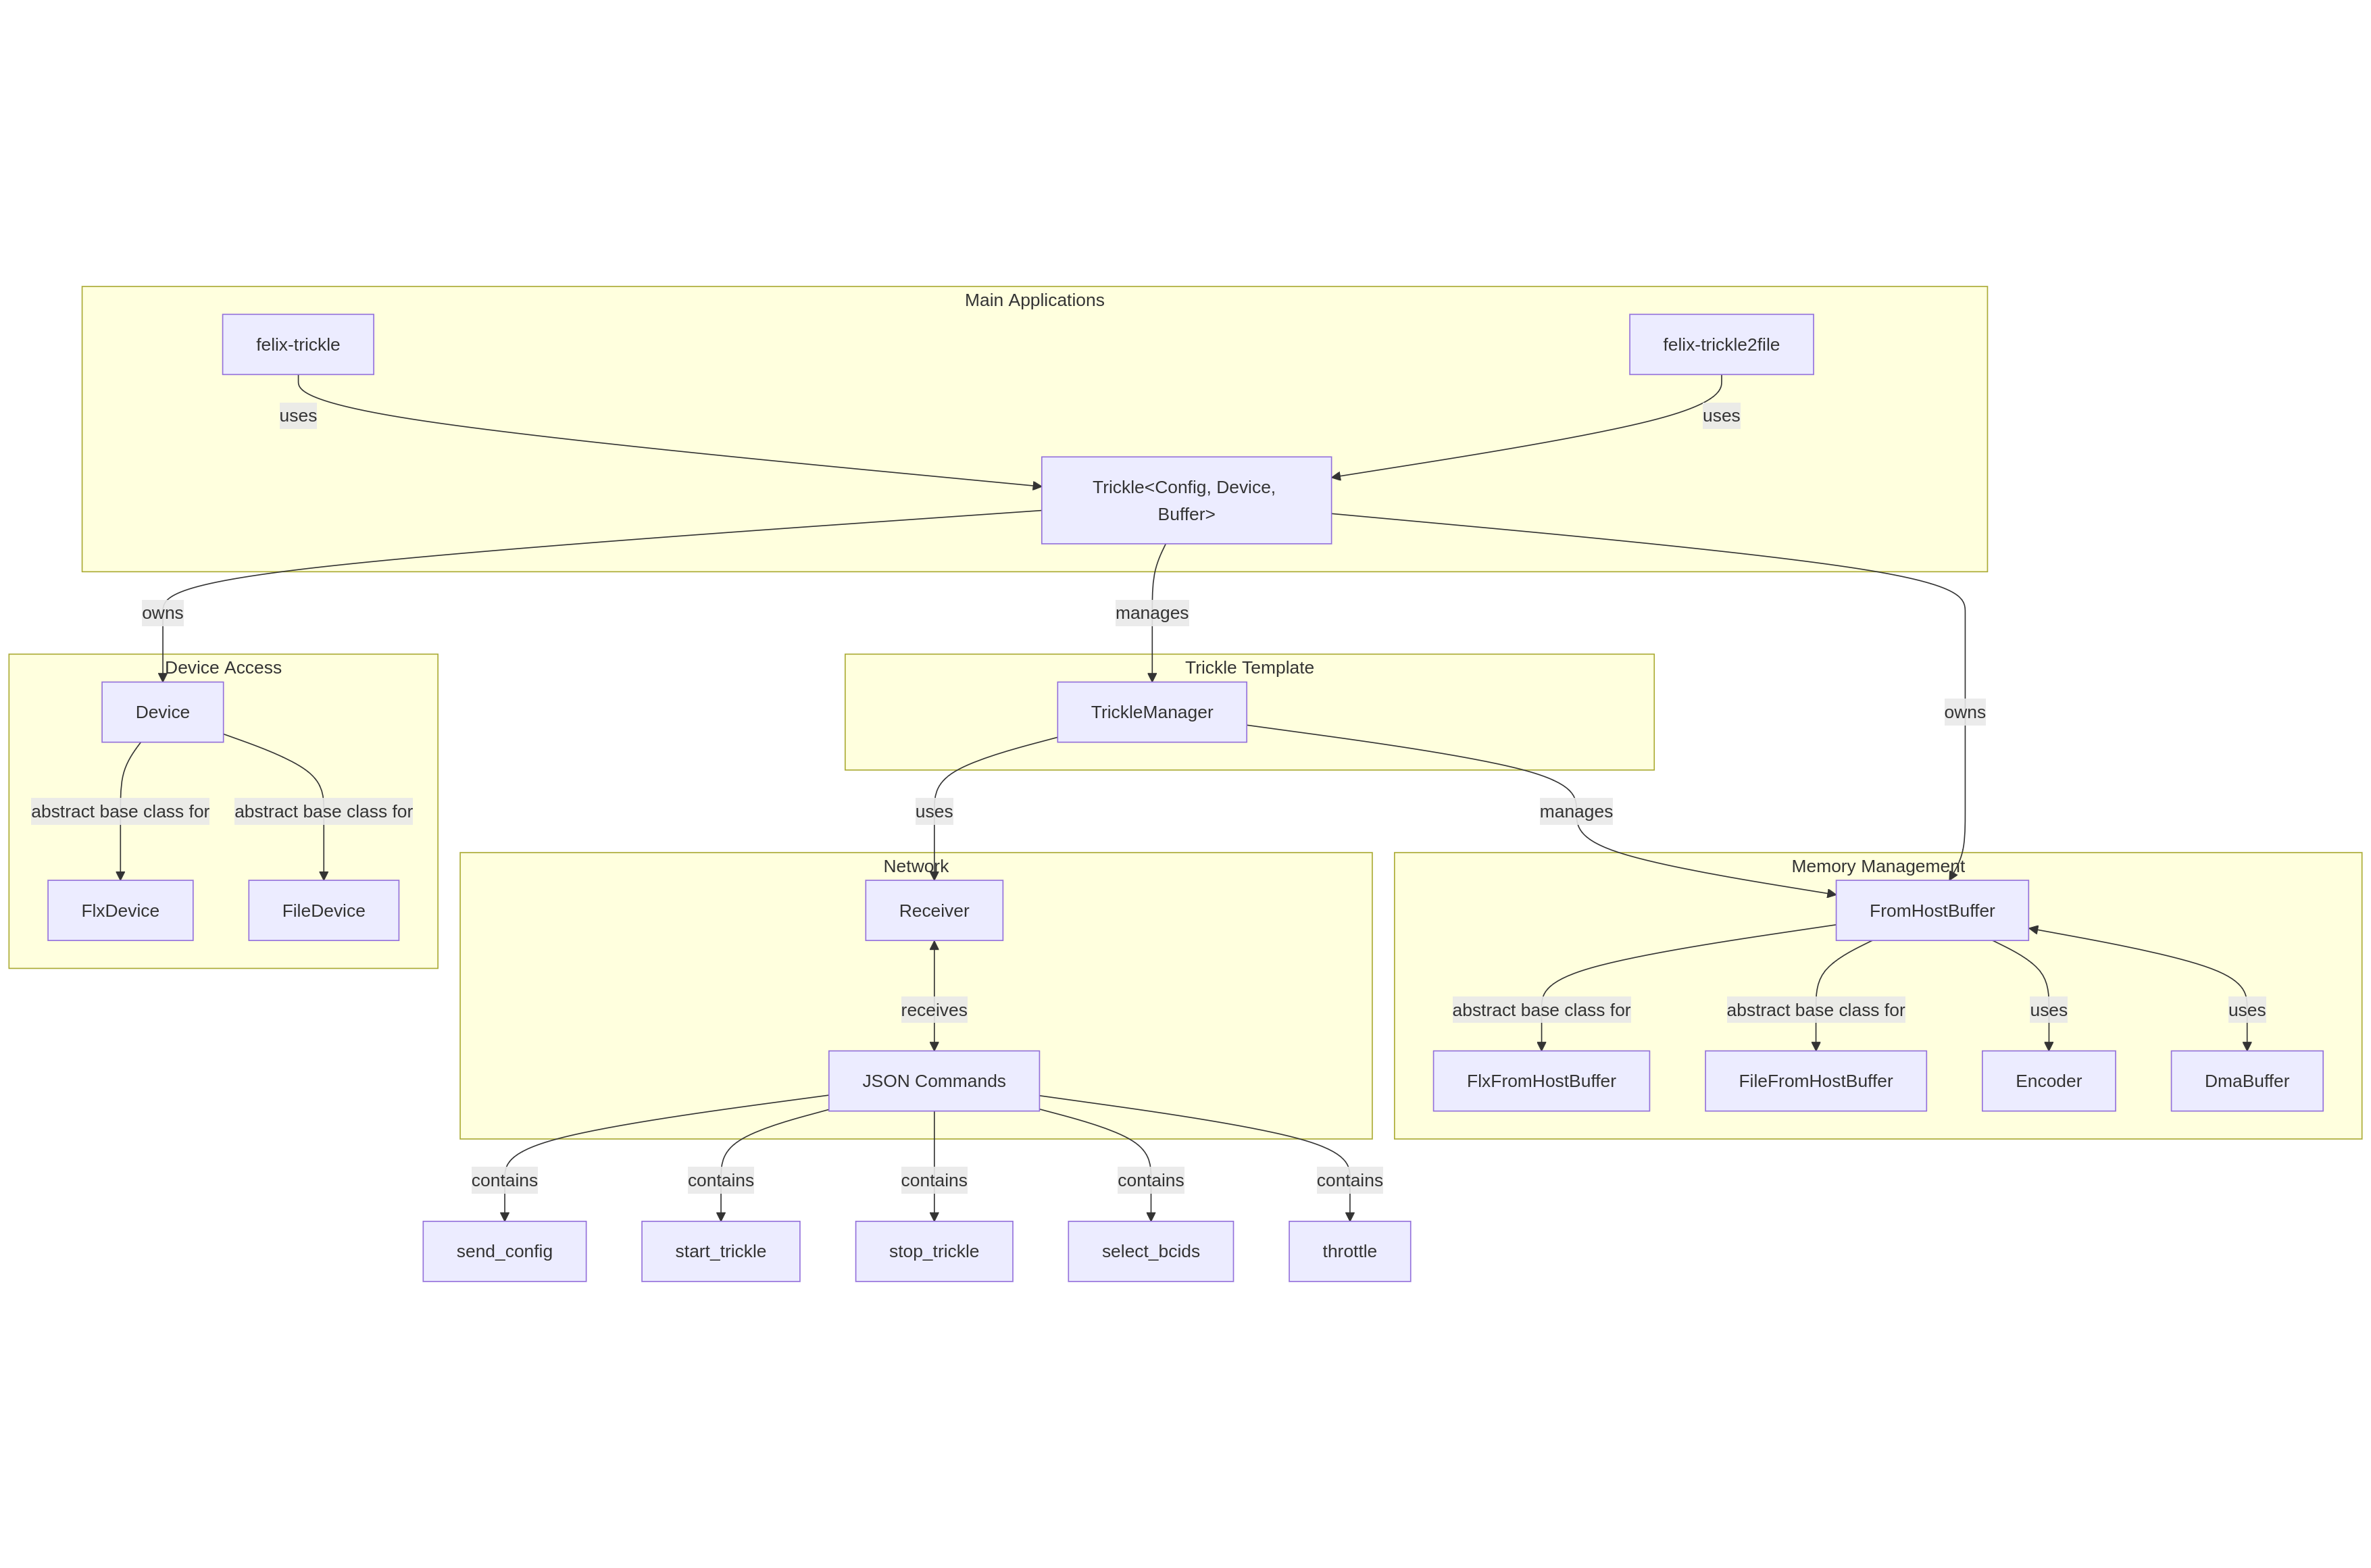
\includegraphics[width=\textwidth]{images/contributions/trickle-architecture.png}
\caption{Software architecture of Trickle configuration.}
\label{fig:trickle-software-architecture}
\end{figure}

\subsection{Software Flow Example}
\begin{enumerate}
    \item Configuration data is received with \textit{send\_config}.
    \item \textit{start\_trickle} starts the "trickling" process.
    \item Host software encodes and writes the payload into the Trickle ring-buffer. The host may add padding for memory alignment (e.g., 4096-byte alignment), a requirement derived from the \acs{PCIe} standard.
    \item Firmware periodically reads from the buffer, sending configuration to the \acs{FE} electronics in between triggers.
    \item \textit{stop\_trickle} stops the "trickling" process.
\end{enumerate}

\subsubsection{felix-trickle} is the name of the main executable (the source file is main\_trickle.cpp) that runs \texttt{trickle\ configuration} on a \acs{FELIX} card. It is responsible for instantiating a \emph{Trickle} instance with the configuration parameters, all the \acs{FELIX} devices installed on the host, and the \acs{DMA} buffers that will be written by the software and read by the firmware. It is responsible for starting or stopping the trickling process through the \emph{Trickle} instance, and for capturing and handling any kernel signals.

\subsubsection{felix-trickle2file} is the name of the main executable (the source file is main\_trickle2file.cpp) that runs \texttt{trickle configuration} in a simulated environment. It is used for regression testing and debugging purposes. It is responsible for instantiating a \emph{Trickle} instance with the configuration parameters, all the emulated \acs{FELIX} devices, and the \acs{DMA} buffers that in this case will be read by an emulator of the firmware and, if the user configured it, written to a file. It is responsible for starting or stopping the emulated trickling process through the \emph{Trickle} instance, and for capturing and handling any kernel signals.

\subsubsection{Trickle} is the class that depending on the configuration parameters and the type of \acs{FELIX}, will be able to perform the trickling operation with the real hardware or an emulated one. It owns, by composition, \acs{FELIX} devices and \acs{DMA} buffers.\\
It is responsible for setting the correct data format with which to fill the \acs{DMA} buffers, to actually allocate the memory for the \acs{DMA} buffers, to publish the data into the \emph{felix-bus} so that the \emph{felix-clients} can communicate with the application, and finally to instantiate a \emph{TrickleManager} instance for each \acs{FELIX} device and a \emph{Receiver} per buffer.

\subsubsection{TrickleManager} is the class that implements the \acs{API} that allows to use \texttt{trickle configuration}. The \acs{API} is composed of the following functions:
\begin{itemize}
    \item \texttt{send\_config}: Sends the configuration data to the \acs{FELIX} card.
    \item \texttt{start\_trickle}: Starts the trickling process.
    \item \texttt{stop\_trickle}: Stops the trickling process.
    \item \texttt{select\_bcids}: Selects the bunch crossing IDs in which to send the config messages.
    \item \texttt{throttle}: Throttles the trickling process.
\end{itemize}

It uses a \texttt{Receiver} (Subsection~\ref{subsubsec:receiver}) to receive commands in JSON format from a client, and each command uses one of the aforementioned functions.\\

\texttt{select\_bcids} merits some explanation. In the \acl{LHC} there are two directions in which particles can circle; the particles are divided in "bunches" inside a beam, the collisions happen always between the same bunches in the crossing points that correspond to the four experiments presented in the introduction~\ref{sec:lhc-experiments}, and this collision will have an ID which is the \acl{BCID}. \emph{Trickle configuration} is supposed to send data in between triggers, which happen when the bunches cross, so with \emph{select\_bcids} one can theoretically select only the IDs preceding longer periods without collisions. The effect of selecting \acs{BCID}s is that of throttling, for which there is a function implemented in the \acs{API}, but both of them have been kept since they are two different concepts even though they have the same final effect.\\
A reference to a tool to simulate bunch crosses inside the \acs{LHC} \cite{bunch-crossing-tool}.

There are private implementations of the callback functions that are used to handle the events of opning/closing a connection and receiving data. There is also a function that adds padding to a \emph{trickle configuration} payload to ensure that the data is aligned to a 4096-byte boundary, which is a requirement of the latest \acs{PCIe} standard. The interesting part is that the padding needs to actually be a valid message for the firmware to be able to read it. The final implementation consists on adding a header that contains a valid \acs{E-link} but an invalid E-path. Following this change, the firmware has been developed to simply ignore and discard messages with headers containing invalid \acs{E-link}s.

\subsubsection{FromHostBuffer} is the abstract base class that is tasked with managing buffers in the \texttt{felix-toflx} direction. It is specialized to work both with the real hardware and with the emulated one. It is responsible keeping track of the read and write pointers to the \acs{DMA} buffer it is wrapping, and to manage concurrent \emph{write} and \emph{read} operations to it.

\subsubsection{Device} is the abstract base class that represents a \acs{FELIX} device. It is responsible for managing the connection to the \acs{FELIX} card, and for providing an interface to read and write registers. It is specialized to work both with the real hardware (one object = one \acs{PCIe} endpoint) or to emulate one. The class is used by \emph{TrickleManager} to access the \acs{FELIX} card or the emulated one.\\

\subsubsection{Receiver} \label{subsubsec:receiver} is the interface implemented by the network backed that the trickle software uses to receive data from the network.

\subsection{Firmware's role}

The \acs{FELIX} firmware is responsible for reading configuration data from the Trickle buffer and forwarding it to the appropriate \acs{FE} links. The read pointer in firmware advances as configuration data is consumed. No write pointer is maintained in firmware; the reason behind the pointers choice is because \textit{trickle configuration} is something that will not change often, it is meant to be written one time in the \acs{DMA} buffer with the firmware continuously reading the buffer and sending the configuration in between triggers. When the configuration needs to change, the buffer is set to one-shot (which invalidates the buffer once reading the last bit), the confiuration is changed, the buffer is again set to be a ring-buffer and the firmware is given the signal to start reading again by setting the register that validates the buffer.\\
The firmware is implemented in a way so that \texttt{trickle configuration} has the lowest priority compared to other data.

\subsection{Trickle Configuration - Client}

Image~\ref{fig:trickle-client-uml} how the \texttt{Trickle Configuration} \acs{API} call has been implemented on the client side \cite{felix-star-trickle-client}. 

\begin{figure}[htbp]
\centering
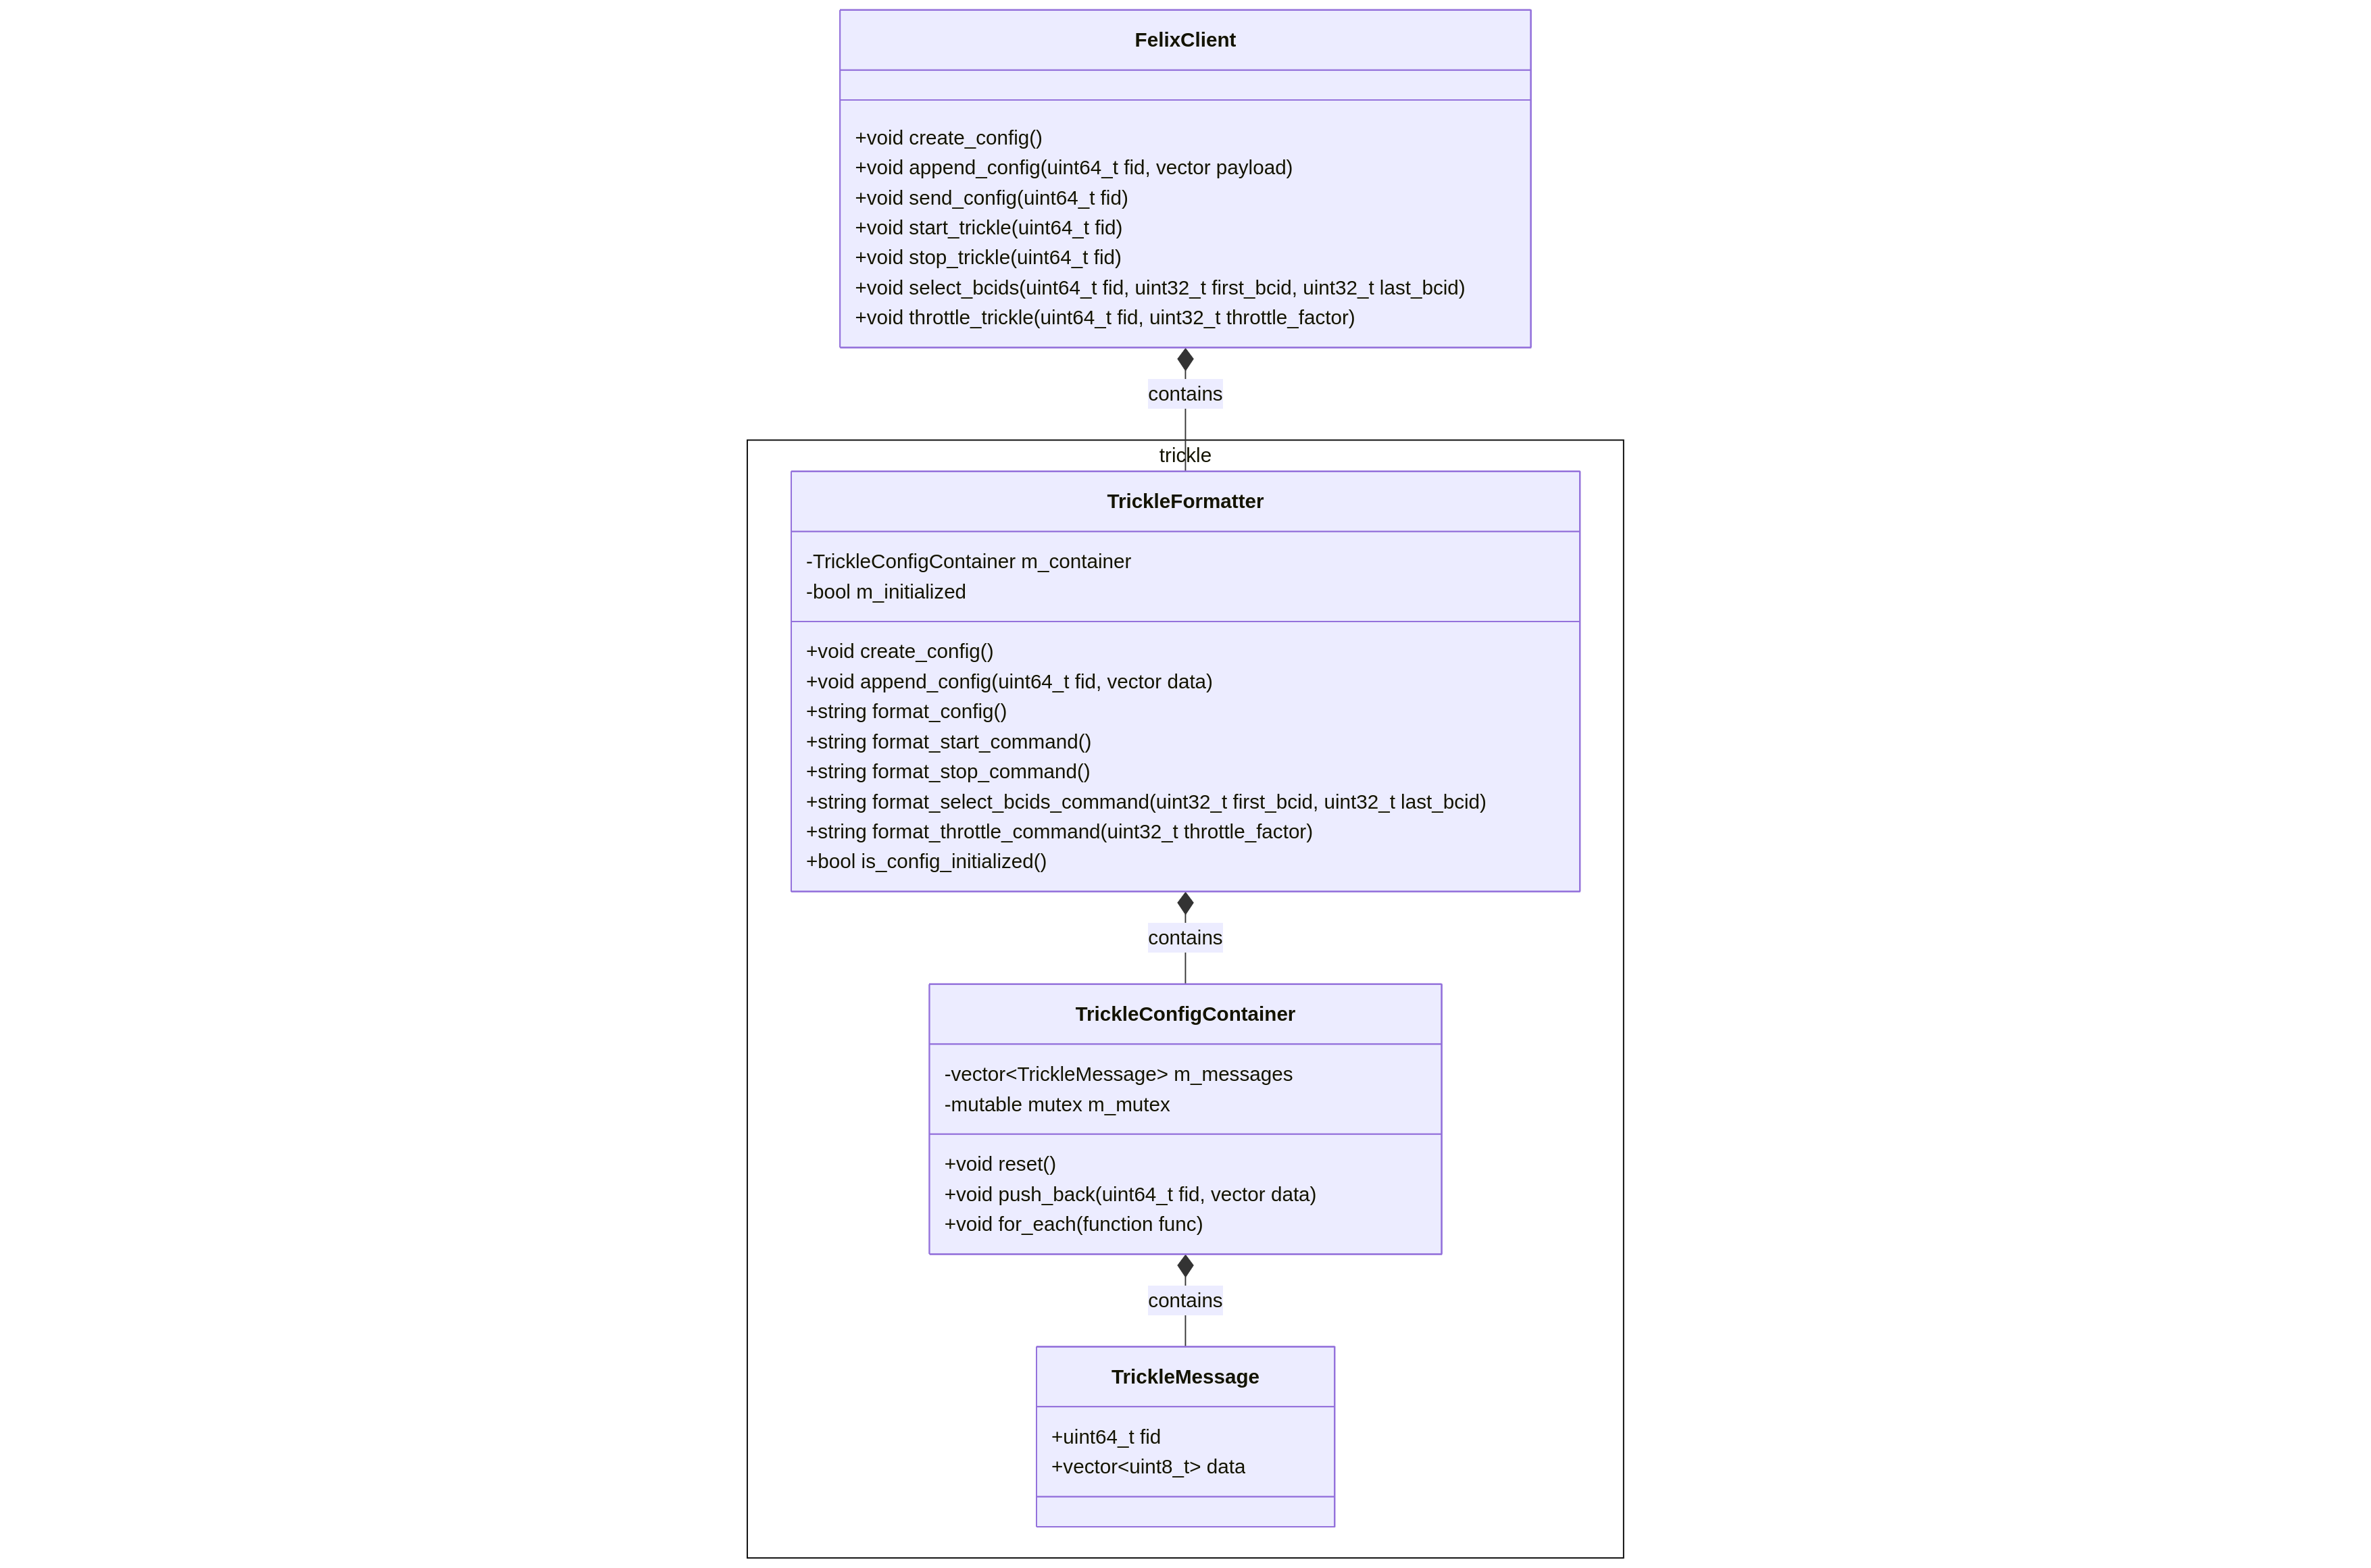
\includegraphics[width=\textwidth]{images/contributions/client-trickle-config-uml.png}
\caption{UML diagram Trickle Configuration in the client side.}
\label{fig:trickle-client-uml}
\end{figure}

A brief explanation of the classes involved in the client-side implementation of the \texttt{Trickle Configuration} \acs{API}:

\begin{itemize}
    \item \textbf{TrickleMessage}: An internal structure that represents a single Trickle configuration message. It contains the \acs{FID} and the payload.
    
    \item \textbf{TrickleConfigContainer}: A container for \texttt{TrickleMessage} structs. Its role is to provide a thread-safe storage and manipulation of trickle messages.
    
    \item \textbf{TrickleFormatter}: This class is responsible for formatting trickle messages into JSON strings.
    
    \item \textbf{FelixClient}: This is the class that implements the \acs{API} to interact with the \texttt{felix-star} applications. It is responsible for sending and receiving messages, and for managing the connection to the \texttt{felix-star} applications. In the context of \texttt{trickle configuration} it uses the \texttt{TrickleFormatter} generate trickle configurations in JSON format, and generate commands to send to the server, also as JSON strings.
\end{itemize}

\clearpage
\subsection{Monitoring - Software Architecture}

Initially, the \acs{FELIX} monitoring system was structured around a \texttt{Monitor} class, which provided a \texttt{write\_message()} method. This method was inherited and overridden by subclasses such as \texttt{FromHostMonitor} and \texttt{ToHostMonitor}. While this approach allowed for some specialization, it tightly coupled the monitoring logic with the output mechanism, making it difficult to introduce new output formats or destinations without modifying the core monitoring classes.

To address these limitations, the architecture was refactored to apply the \textit{Strategy design pattern}. Figure~\ref{fig:monitoring-software-architecture} shows a UML diagram of the most important parts composing the \textit{Monitoring} implementation; a complete UML diagram is in Figure~\ref{fig:complete-monitoring-uml}. The Strategy pattern allows selecting an algorithm's behavior at runtime by encapsulating it within a separate class and delegating the execution to that class.

\begin{figure}[htbp]
\centering
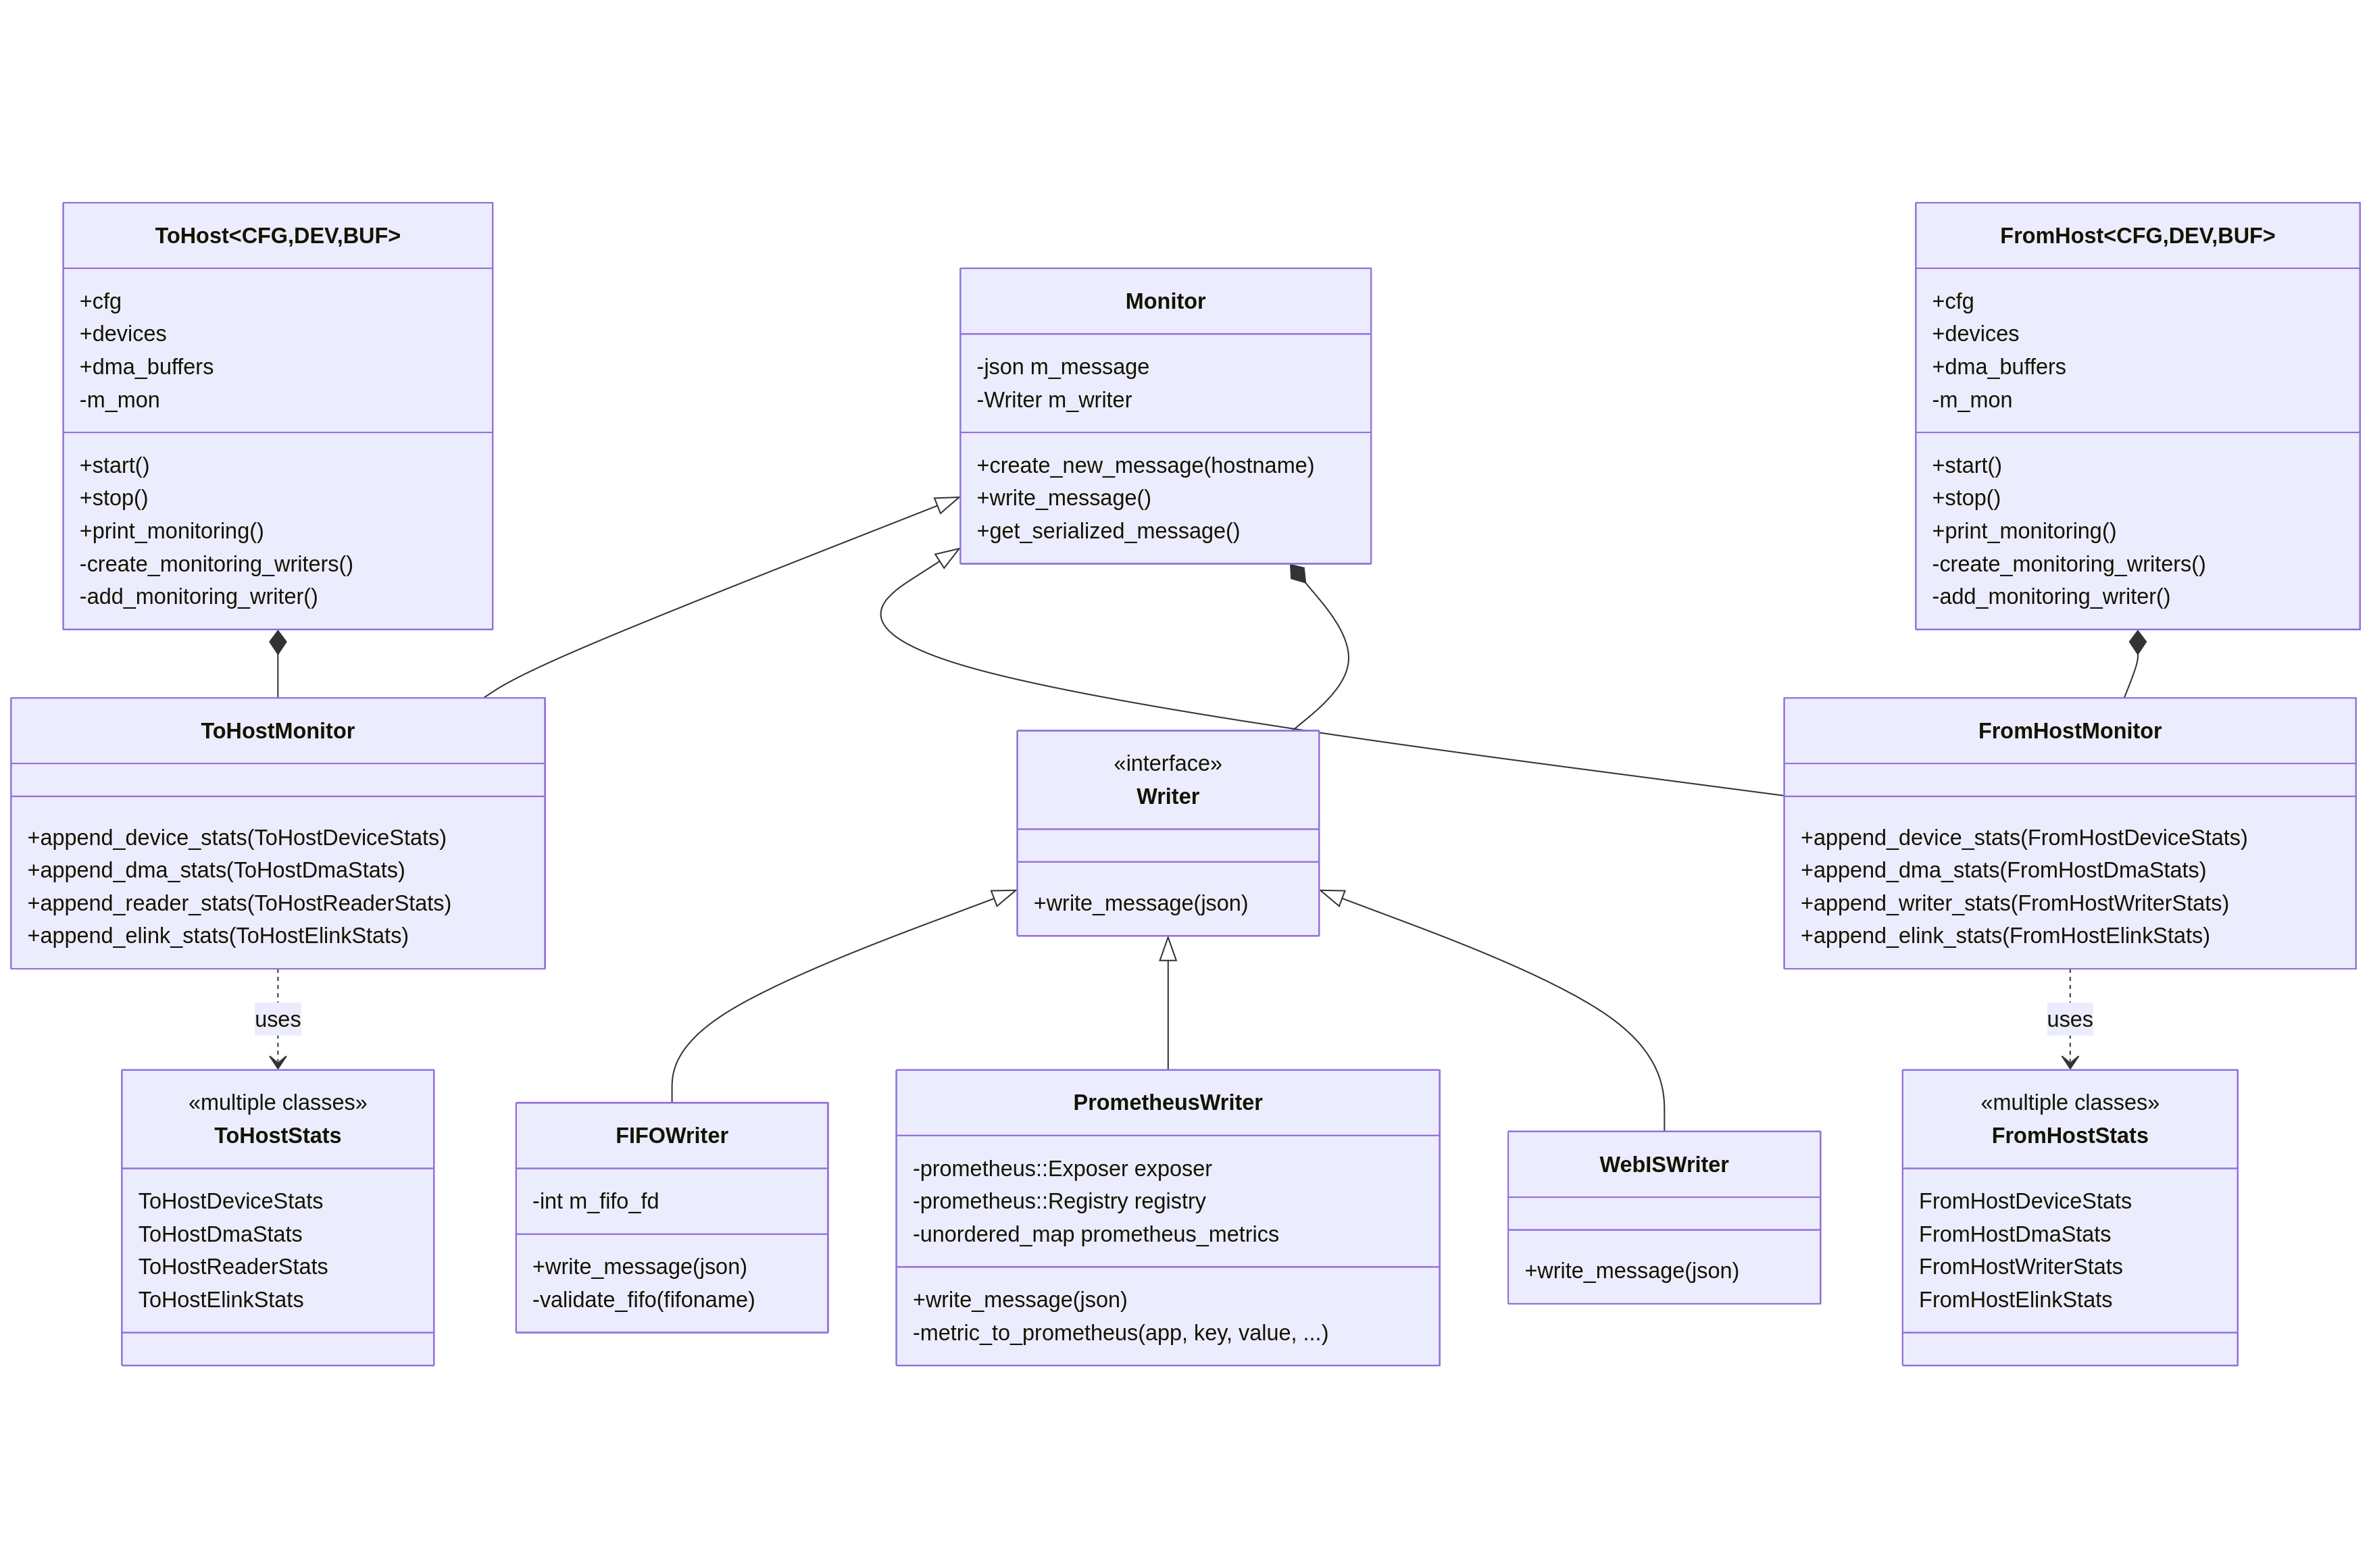
\includegraphics[width=\textwidth]{images/contributions/monitoring-uml.png}
\caption{Overview of the monitoring software architecture.}
\label{fig:monitoring-software-architecture}
\end{figure}

\textbf{Monitor} is the class that is used by the \texttt{felix-star} applications to produce monitoring data. It is an abstract base class that defines the interface for monitoring. It has a pure virtual method \texttt{write\_message(const nlohmann::json\&)} that must be implemented by subclasses. The \texttt{Monitor} class is responsible for collecting monitoring data and delegating the writing of that data to a \texttt{Writer} instance. The concrete implementations are defined depending on the direction, thus there are \emph{ToHostMonitor} and \emph{FromHostMonitor}. The choice of the \texttt{Writer} implementation is determined at runtime based on user configuration, allowing the same monitoring logic to be reused with different output strategies.

\textbf{Writer} is the abstract base class for the three concrete implementations of the monitoring output strategies. Each of the concrete classes implements the \texttt{write\_message(const nlohmann::json\&)} method, which defines how the monitoring data is written to the desired output or destination. The concrete implementations of this class include:

\begin{itemize}
    \item \textbf{FIFOWriter}: Writes monitoring data to a UNIX FIFO (Figure~\ref{fig:fifo-monitoring}).
    \item \textbf{PrometheusWriter}: Exposes metrics in a format consumable by Prometheus (Figure~\ref{fig:felix-tohost-monitoring}, Figure~\ref{fig:felix-tohost-single-elink}).
    \item \textbf{WebISWriter}: Used to send monitoring data to \acs{IS}, a monitoring tool used internally in \acs{ATLAS} (Figure~\ref{fig:felix-tohost-is}).
\end{itemize}

\clearpage

\begin{figure}[H]
\centering
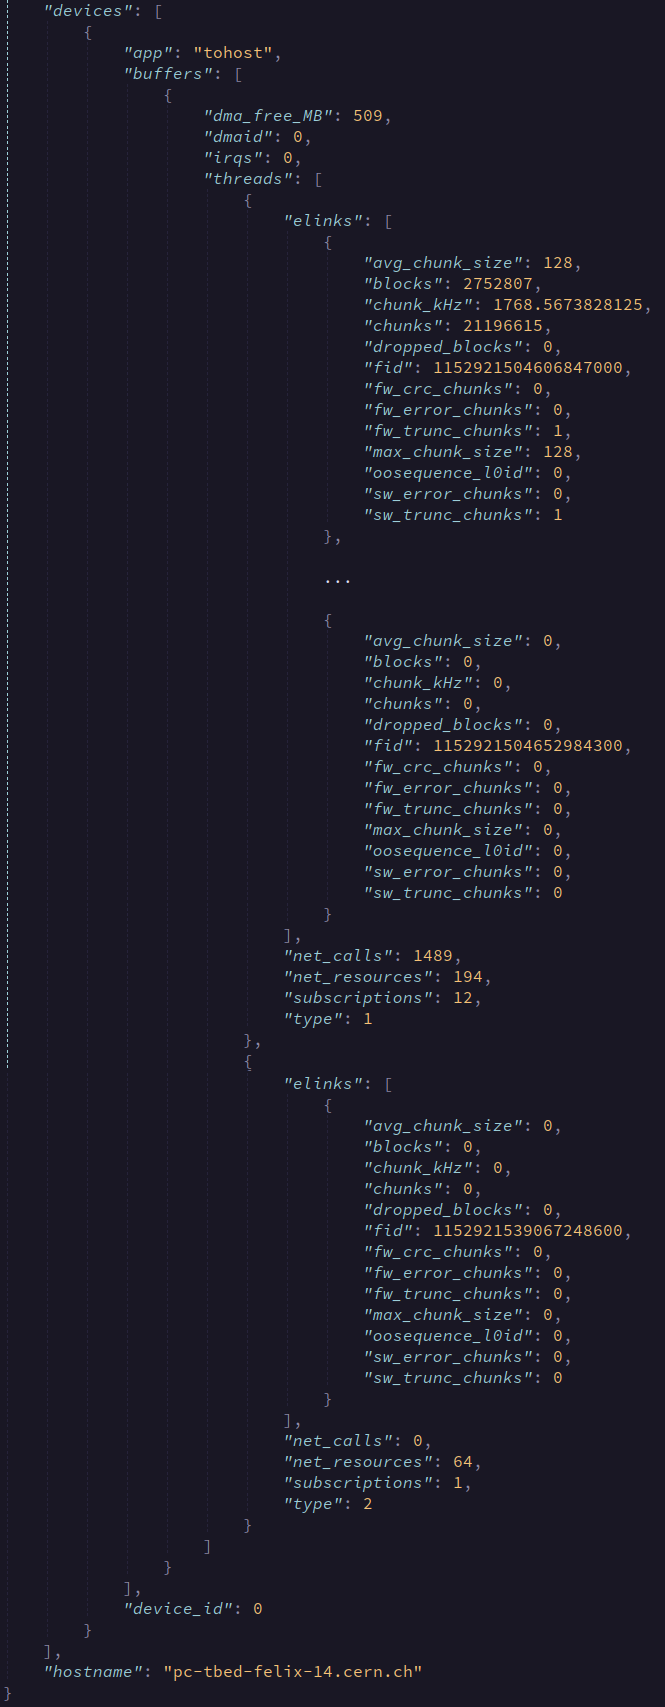
\includegraphics[width=0.46\textwidth]{images/results/fifo-monitor.png}
\caption[Monitoring FIFO example]{An example of what can be seen inside the UNIX FIFO. It's a JSON message containing the monitoring data.}
\label{fig:fifo-monitoring}
\end{figure}

\begin{figure}[H]
\centering
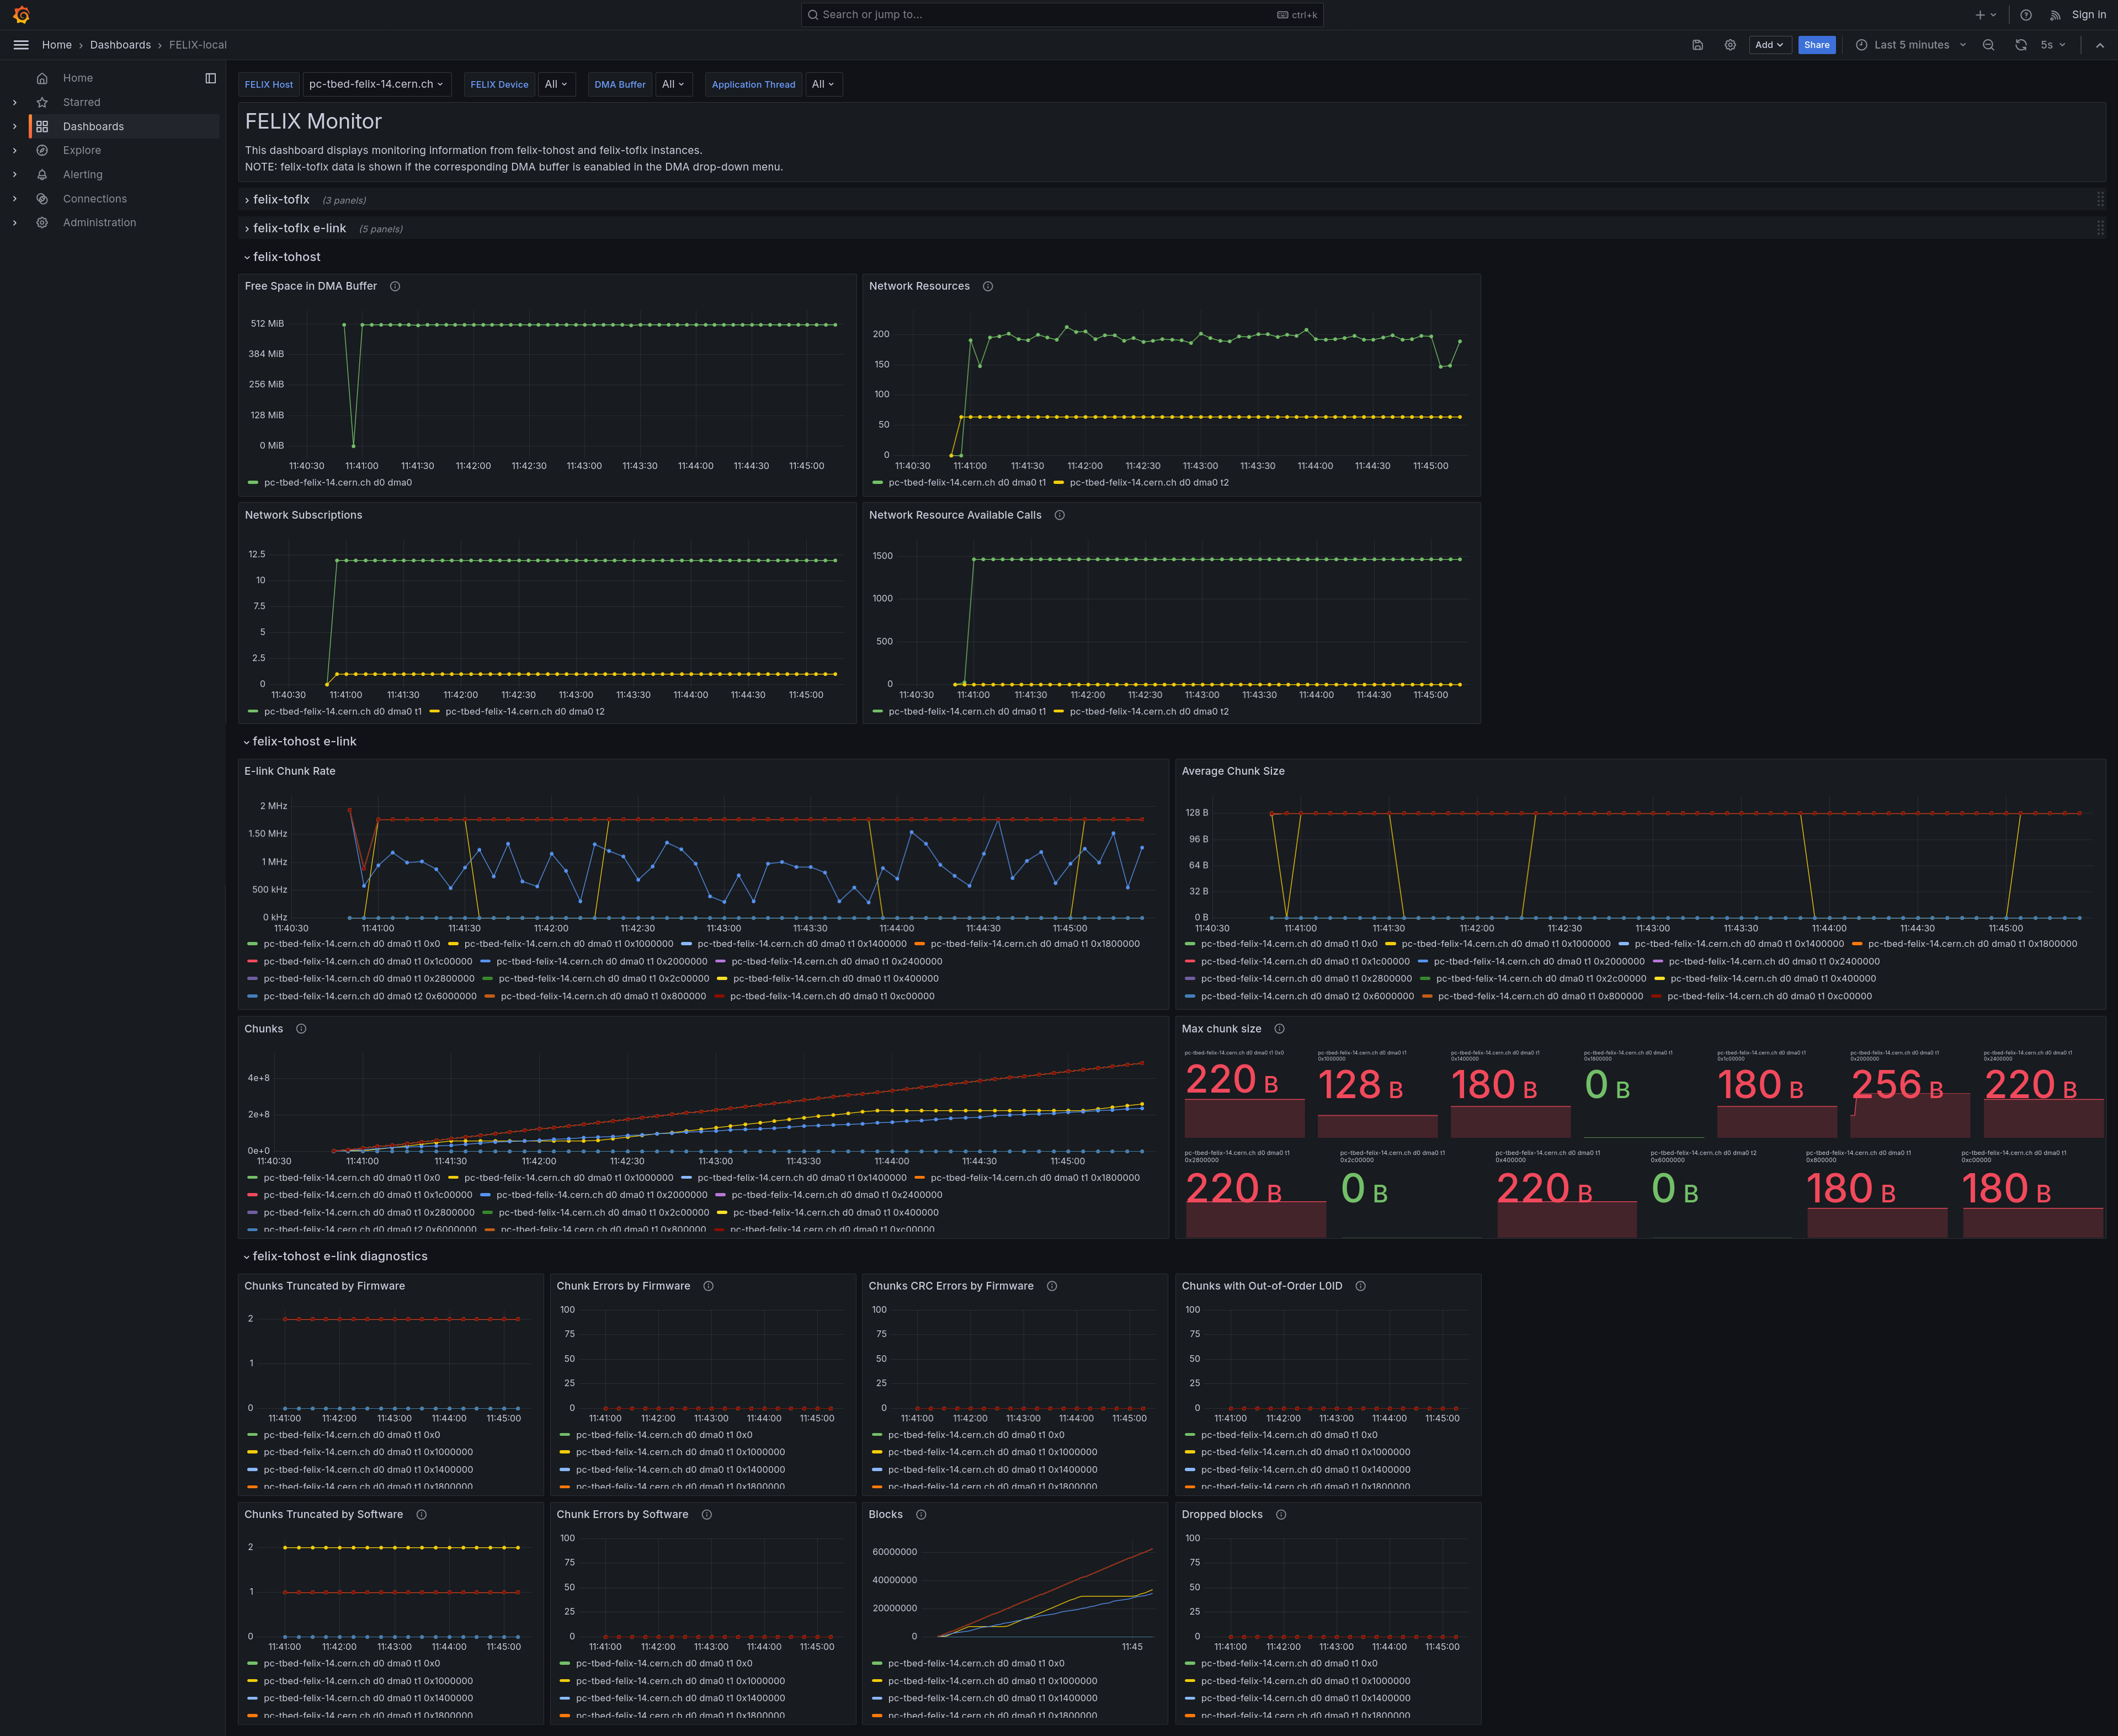
\includegraphics[width=\textwidth]{images/results/monitoring-merged.png}
\caption[Grafana sample screenshot]{This is a sample screenshot of the combined Prometheus and Grafana solution. The sampling rate can be set in the docker image, in this case it is 5 seconds. Here, I was stress testing felix-tohost as shown by the size of the chunks and their \acs{E-link} rate well above 1.5 MHz. }
\label{fig:felix-tohost-monitoring}
\end{figure}

\begin{figure}[H]
\centering
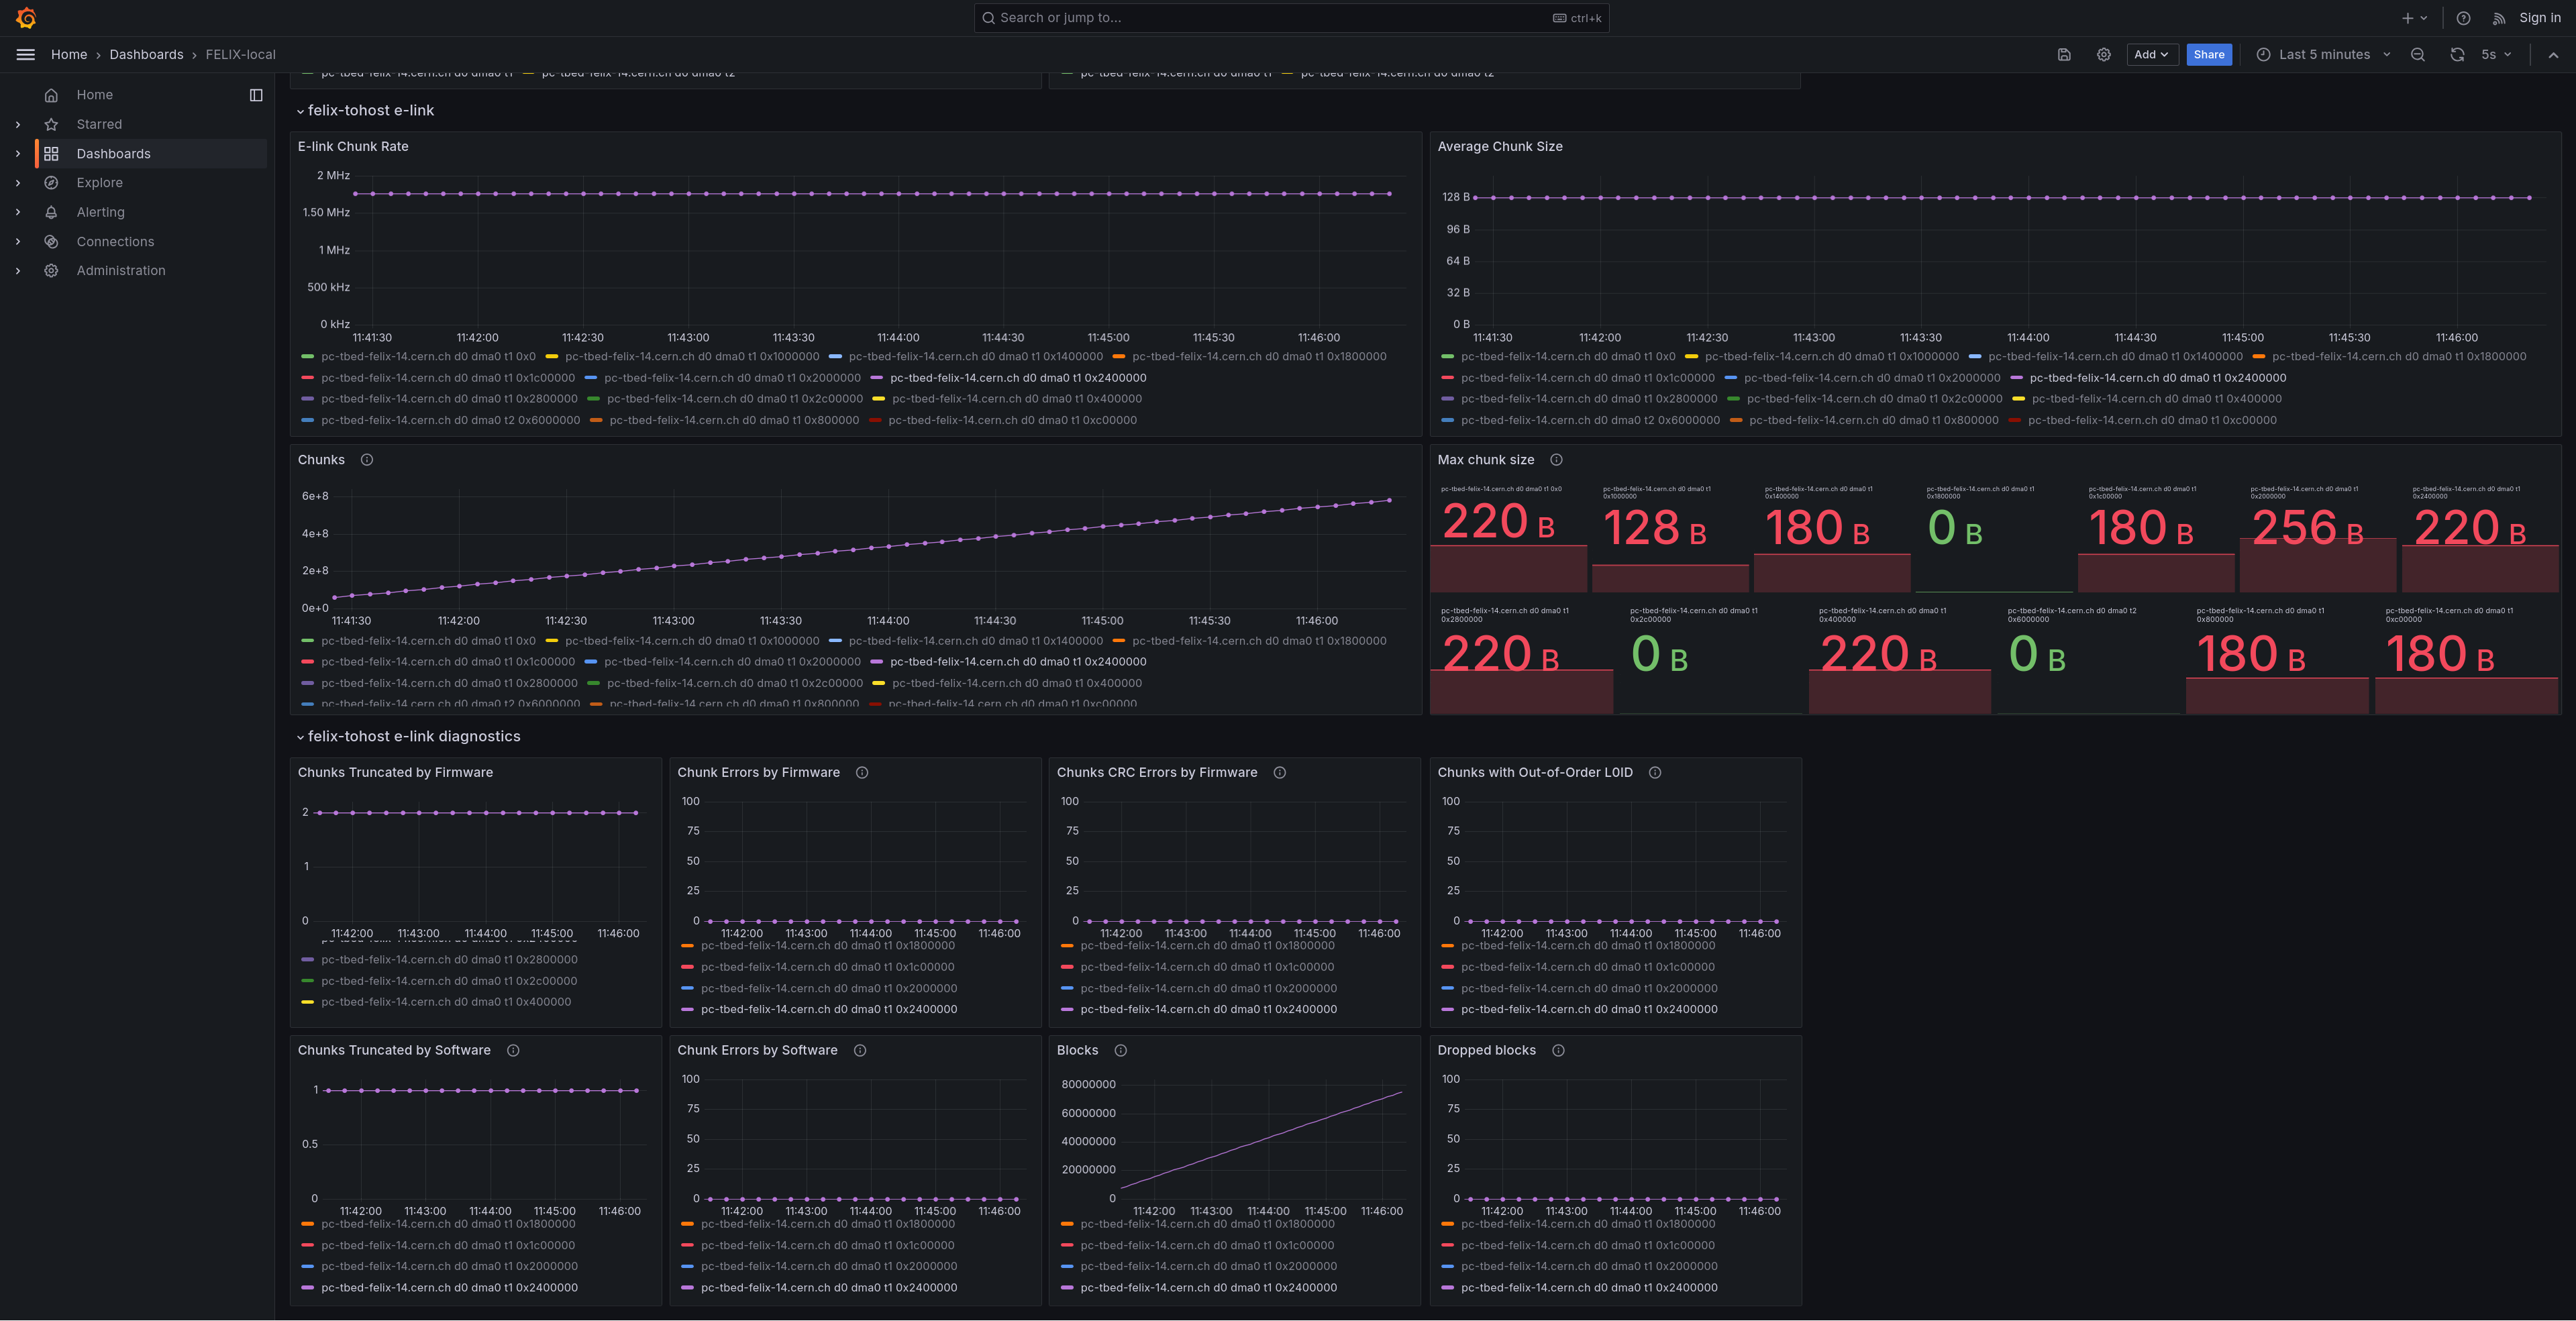
\includegraphics[width=\textwidth]{images/results/monitor-one-elink.png}
\caption[Grafana screenshot: select one E-link]{Here is shown that it is possible to select and focus one element at a time, in this case I selected the \acs{E-link} 0x2400000.}
\label{fig:felix-tohost-single-elink}
\end{figure}

\begin{figure}[H]
\centering
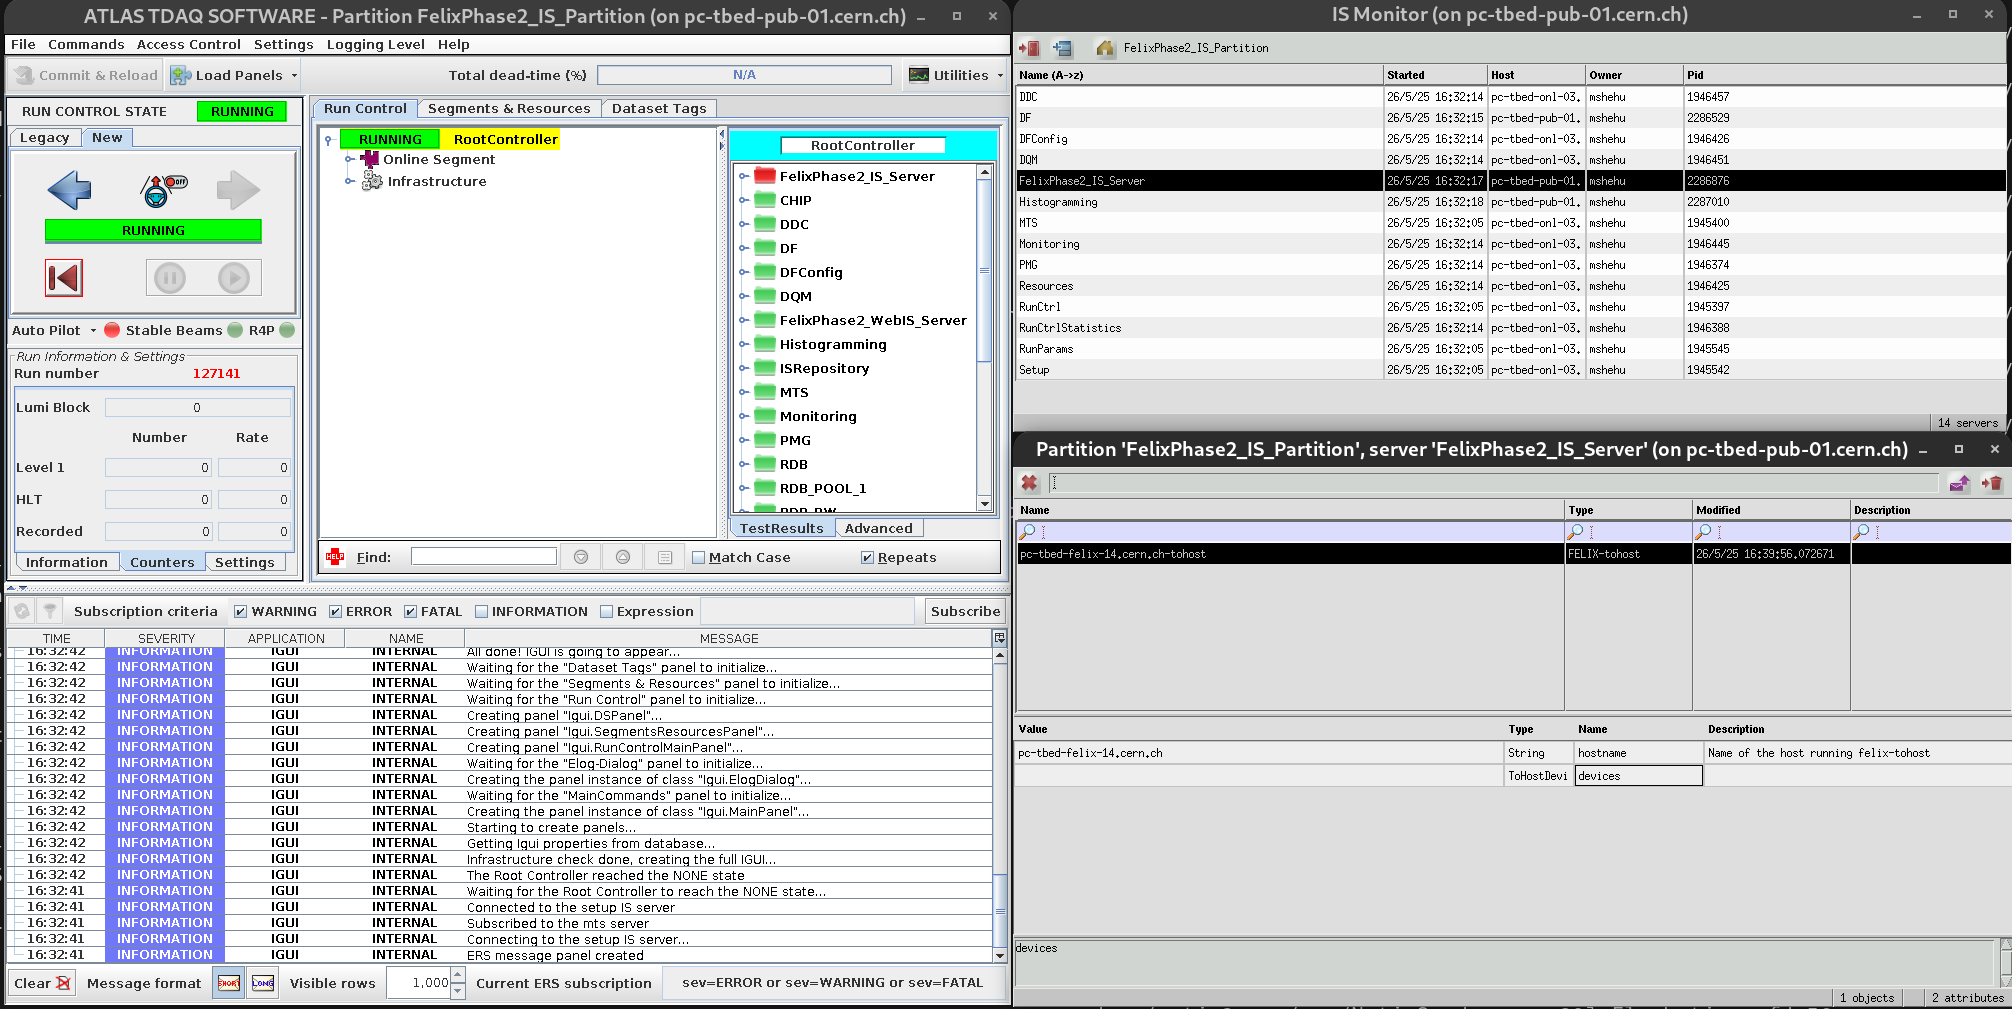
\includegraphics[width=\textwidth]{images/results/IS-monitoring.png}
\caption[IS monitoring screenshot]{Sample image with IS monitoring. The reason that it is red is because it's trying to test it but there is no test available since this is just a play setup to check if it works.}
\label{fig:felix-tohost-is}
\end{figure}


\subsection{Migration of the logging system from clog to ERS}

The contribution in this matter is straightforward: the logging system has been migrated from \texttt{clog} to \texttt{ERS}. The purpose of this migration is to make \texttt{felix-star} consistent and coherent with the \acs{ATLAS} \acs{T-DAQ} software ecosystem \cite{felix-star-clog-to-ers}.\\
Contrary to the approach of other software using ERS, for \texttt{felix-star} I decided to create a general issue per Class, and specialize the issue with a custom message depending on the situation.\\
Below an Example~\ref{lst:ers-example} of an actual implementation:

\begin{lstlisting}[language=C++, caption={Example of ERS custom issue declaration and usage.}, label={lst:ers-example}]
/* In the header file */
// Declare a custom issue for logging configuration-related errors
ERS_DECLARE_ISSUE(felix_log, device_flx_issue, issue_message, ((const
std::string&)issue_message))

/* In the cpp file */
// Use the custom issue to log an error
ers::error(felix_log::device_flx_issue(std::format("Invalid encoding type {}
for elink channel {} group {}, epath {} using DIRECT", enc, channel, egroup,
epath)));
;
\end{lstlisting}
\chapter{Netio3}
\label{chap:netio3}

Netio3 \cite{netio3-docs} is a transport-agnostic networking library originally created for the Phase-2 \acs{FELIX} system, offering both TCP and \acs{RDMA} communication pathways.  It is organized into two modules: the \texttt{netio3-backend} and the \texttt{netio3-frontend}.  The backend is responsible for data transmission and reception over the network and does not contain any \acs{FELIX}-specific logic, making it reusable in other projects. The frontend builds on this by providing buffered I/O for efficient data coalescence, a publish/subscribe API and data formatting.  Under the hood, TCP transport is implemented by the \acs{ATLAS} \acs{T-DAQ} \texttt{asyncmsg} \cite{asyncmsg} library, while \acs{RDMA} operations use the \texttt{libfabric} \cite{libfabric} library.  Both transports follow a connection-oriented, message-based paradigm.

\section{Netio3 backend}

Both the \texttt{asyncmsg} and the \texttt{libfabric} backend use an event-driven model in the form of an event loop. Events can be callbacks from the underlying network library notifying the application about new connections, incoming data or user defined callbacks added through signals and timers. The event loop is single threaded, thus guaranteeing that all events are executed sequentially. Each event is associated with a callback that contains the user code that is executed when the event is triggered.

\subsection{Eventloop implementation}

There are two different event loop implementations: One based on the Linux kernel epoll system call (EpollEventLoop), and one based on Boost::ASIO::io\_service (AsioEventLoop). Both backends (The two versions are described below) are compatible with either event loop implementation. The same event loop can be used to power multiple backends.


\subsection{Libfabric backend}
\label{subsec:libfabric}

\texttt{libfabric} \cite{libfabric} is a library that provides a high-performance, low-latency communication interface for distributed applications. It abstracts the underlying network hardware and protocols, allowing developers to write portable code that can run on different network technologies without worrying about the specifics of the network stack. \texttt{libfabric} is especially useful when there are multiple systems using different network hardware and protocols, like in \acs{ATLAS}, because without it, one would to write separate code for each network type; instead \texttt{libfabric} offers a programming interface called the OpenFabrics Interfaces (OFI). When an application wants to send data, it makes calls to \texttt{libfabric} using this standard interface. \texttt{libfabric} then translates these calls into the specific commands needed for whatever network hardware is actually installed in the system. The library supports various transport protocols, including TCP and \acs{RDMA}.

\subsubsection{Sending data}

\texttt{libfabric} aims to provide maximum performance. One way to achieve high performance is to avoid data copies. This is done by registering memory regions with an \acs{RDMA} device. Memory registration is an operation that basically pins that memory region only for an \acs{RDMA} device, since sending data to an \acs{RDMA} device from outside registered memory regions is not possible. This also requires the guarantee that after initiating a send operation, the data is not modified until the operation is completed.\\

For \texttt{buffered sending}, a given number of buffers is allocated in memory, and then they are registered with \texttt{libfabric}.\\
For memory coherency and to avoid data corruption, a buffer can never be modified after send\_buffer is called and before receiving the completion message. Matching send operations with completions is done internally.

For \texttt{zero-copy sending}, are registered two memory regions: one main memory region containing the data, and one region containing the additional header information (16 bytes per send operation).  Matching the send operations with completions is not supported by the library and has to be managed by the user.

\subsubsection{Receiving data}

As for sending data, receiving data also requires registering memory regions. When data is received, it is placed into an available buffer by the \acl{NIC} and provided to the user via a receive-completion callback. After reading, the buffer is then returned to the \texttt{libfabric} backend and can be used for the next receive operation.\\
For the \texttt{libfabric} backend, opening and closing connections is an expensive operation.

\subsection{Asyncmsg backend}
\label{subsec:asyncmsg}

\texttt{asyncmsg} is a message based wrapper of Boost::ASIO, developed by the \acs{ATLAS} \acs{T-DAQ} group. It provides a high-level interface for asynchronous message passing over TCP/IP networks, allowing applications to send and receive non-blocking messages (what asynchronous means).\\
The \texttt{asyncmsg} backend is thread safe.

\subsubsection{Sending data}

Contrary to the \texttt{libfabric} backend, the data for zero-copy sending in \texttt{asyncmsg} does not have to reside inside a registered memory region.\\
The most practical feature of \texttt{asyncmsg} for sending data is \texttt{immediate sending}, which essentially copies the data into a dynamically allocated buffer and sends it right away. This method does not require the allocation of multiple buffers, imposes no restrictions on data size, and does not require the user to guarantee data stability. However, it is also the slowest method of data transmission. For applications requiring high performance, the \texttt{libfabric} backend is preferred.

\subsubsection{Receiving data}

Also for receiving data the user is not required to register memory regions, thus reducing the memory footprint of the applications. This advantage comes at the cost of performance.\\

\section{Netio3 Frontend}

The netio3 frontend is built on top of netio3 backend to handle communications in a distributed system for data acquisition. The frontend introduces features such as data coalescence, a publish/subscribe \acs{API}, and a buffer formatting mechanism.

\textbf{Data Coalescence} is one of the core features provided by the netio3 frontend, which consists of a buffering layer that aggregates multiple small messages into larger network packets.\\
This feature is useful in scenarios with bursty or fine-grained message patterns, as it averages the cost of network transmission over multiple messages.


\section{Personal Contributions}

\subsection{New network buffer format}

The \texttt{felix-star} application processes uplink data by dividing it into 1\,KB \texttt{blocks}, decoding these blocks, and passing the decoded data to \texttt{netio3}, which adds a header for the remote clients. 
Previously, a fixed 13-byte header was used; for messages of 10 bytes (or smaller), the overhead ratio was inefficient.
The enhancement involved designing a new, more efficient header and updating the encode/decode routines accordingly \cite{netio3-header-commit}.\\

\begin{figure}[htbp]
\centering
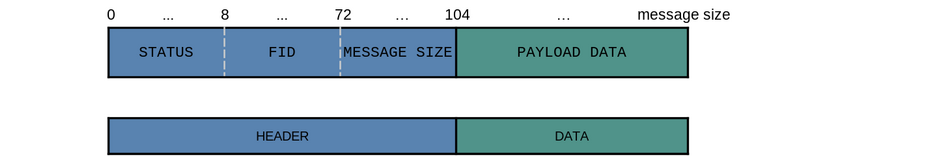
\includegraphics[width=\textwidth]{images/contributions/old-buffer-format.png}
\caption[Legacy format of network buffer]{Legacy buffer format with a 13-byte header. The numbers shown on top are bits}
\label{fig:old-buffer-format}
\end{figure}

\begin{figure}[htbp]
\centering
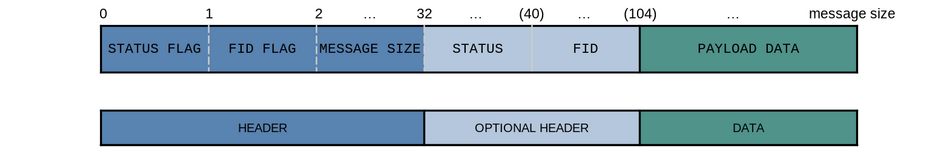
\includegraphics[width=\textwidth]{images/contributions/new-buffer-format.png}
\caption[New network buffer format]{Revised buffer format, reducing header overhead. The numbers shown on top are bits.}
\label{fig:new-buffer-format}
\end{figure}

This optimization works because data in the same \texttt{block} is guaranteed to have the same \acs{FID} since a \texttt{block} is encoded with data coming only from one \acs{E-link}.\\
See Figure~\ref{fig:bock-format} to recall the \texttt{block} format that helps follow the next calculations.\\
Supposing the \texttt{block} is filled, to be conservative with the size, messages of 26 bytes, which is bigger than the size of a typical message coming from \acs{ITk}. A \texttt{block}, as shown in Figure~\ref{fig:bock-format} has always a block-header of 4 bytes (32 bits), and for every other message (\texttt{chunks} and \texttt{subchunks}) there is a header of 4 bytes. With these assumptions a \texttt{block} would contain:
The first header will contain all the optional fields, meaning that the first message will be:
\[
(1024 [\text{bytes}] - 4 [\text{bytes}]) / (26 [\text{bytes}] + 4 [\text{bytes}]) =   34 [\text{messages/chunks}]
\]

\[
(\text{block size} - \text{block header}) / (\text{chunk size} + \text{chunk header}) =   \text{n chunks in a block}
\]

Calculated the number of total 26 byte \texttt{chunks} in a \texttt{block} to be 34, now let's calculate how much space they would occupy once moved into the network buffer with both the old and the new buffer formatting.\\
Starting with the old formatting, every chunck would be preceded by a 13-byte header, wich means that 34 messages into the buffer would occupy:
\[
(13 [\text{bytes}] + 26 [\text{bytes}]) x 34 = 1326 [\text{bytes}]
\]

With the newly implemented buffer formatted, the first message in the buffer would occupy:

\[
13 [\text{bytes}] + 26 [\text{bytes}] = 39 [\text{bytes}]
\]

The next headers are guaranteed to have the same \acs{FID}, so the would occupy:
\[
(4 [\text{bytes}] + 26 [\text{bytes}]) x 33 = 990 [\text{bytes}]
\]

Making the total occupancy for the new format:
\[
39 [\text{bytes}] + 990 [\text{bytes}] = 1029 [\text{bytes}]
\]

In a conservative scenario with the new formatting, the network buffer would occupy $\approx$\text{25\%} less space.
\chapter{Results}

\section{Hardware testing}

A total of 40 FLX-182-1B cards, in 3 different batches, were subjected hardware validation and testing. During this process, 10 cards were found to be non-functional due to a range of issues, including component failures and configuration errors. Through the aformentioned diagnostics and interventions, 8 of the faulty cards were fully or partially recovered and restored to operational status.\\
All the recovered cards are now delivered to the institutes and functioning properly.

\section{Performance measurements: netio3}
\label{sec:netio3-perf}
The network performance evaluation focused on two key parameters: Throughput and \ac{RTT}. The experiments were conducted in a controlled testbed environment using servers connected via a 200 Gbit/s Ethernet link. The hardware specifications of the servers are detailed below:

\clearpage
\begin{lstlisting}[caption={Network interface information}, label={lst:network}]
[mshehu@pc-tbed-felix-15 ~]$ lspci | grep -E -i --color 'network|ethernet'
41:00.0 Ethernet controller: Mellanox Technologies MT2910 Family [ConnectX-7]
41:00.1 Ethernet controller: Mellanox Technologies MT2910 Family [ConnectX-7]
81:00.0 Ethernet controller: Intel Corporation Ethernet Controller X550 (rev 01)
81:00.1 Ethernet controller: Intel Corporation Ethernet Controller X550 (rev 01)
\end{lstlisting}

\begin{lstlisting}[caption={CPU information}, label={lst:cpu}, float=htbp]
[mshehu@pc-tbed-felix-15 ~]$ lscpu
Architecture:             x86_64
  CPU op-mode(s):         32-bit, 64-bit
  Address sizes:          52 bits physical, 57 bits virtual
  Byte Order:             Little Endian
CPU(s):                   64
  On-line CPU(s) list:    0-63
Vendor ID:                AuthenticAMD
  Model name:             AMD EPYC 9354P 32-Core Processor
    CPU family:           25
    Model:                17
    Thread(s) per core:   2
    Core(s) per socket:   32
    CPU max MHz:          3799.0720
    CPU min MHz:          1500.0000
\end{lstlisting}

\clearpage
\begin{lstlisting}[caption={Memory information}, label={lst:memory}]
[mshehu@pc-tbed-felix-15 ~]$ lsmem
RANGE                                 SIZE  STATE REMOVABLE BLOCK
0x0000000000000000-0x000000187fffffff  98G online       yes  0-48
\end{lstlisting}

The receiving machine was equipped with an older FLX-712 card, while the sending machine utilized the new FLX-182-1B prototype developed for Phase II. This emulates the \texttt{felix-tohost} direction. The statics have been collected from the sending part; the reason was because the sending part interrupts the connection, and the statistics collection could be stopped at the same time.

The throughput tests were conducted using the two \textit{netio3-backends} LIBFABRIC-RDMA and ASYNCMSG-TCP. To manage the high number of tests, an Ansible \cite{ansible} playbook was developed. The output of the playbook was processed using a custom Python script, which also generated the graphs using the Matplotlib \cite{matplotlib} library. The tests involved varying the buffer size --- ranging from 1 KB to 64 KB  (in ATLAS production are used buffers of 64 KB) --- and the number of buffers. The same buffer size and number of buffers were used for both the sender and receiver. 

The sender transmits buffers sequentially, employing a polling mechanism to determine when the next buffer could be sent. The receiver, in turn, simply ackowledges and discards the incoming messages without further processing, as the primary objective was to measure throughput. A total of 70 combinations of buffer sizes and counts were tested for LIBFABRIC-RDMA, while only 28 combinations were evaluated for ASYNCMSG-TCP due to diminishing returns observed in preliminary tests.

\subsection{Analysis}

Figures \ref{fig:1kb-buffer-throughput} and \ref{fig:64kb-buffer-throughput} shows the measurements for the two extreme cases: a 1 KB buffer and a 64 KB buffer.

\begin{figure}[htbp]
\centering
\begin{subfigure}[b]{0.7\textwidth}
    \centering
    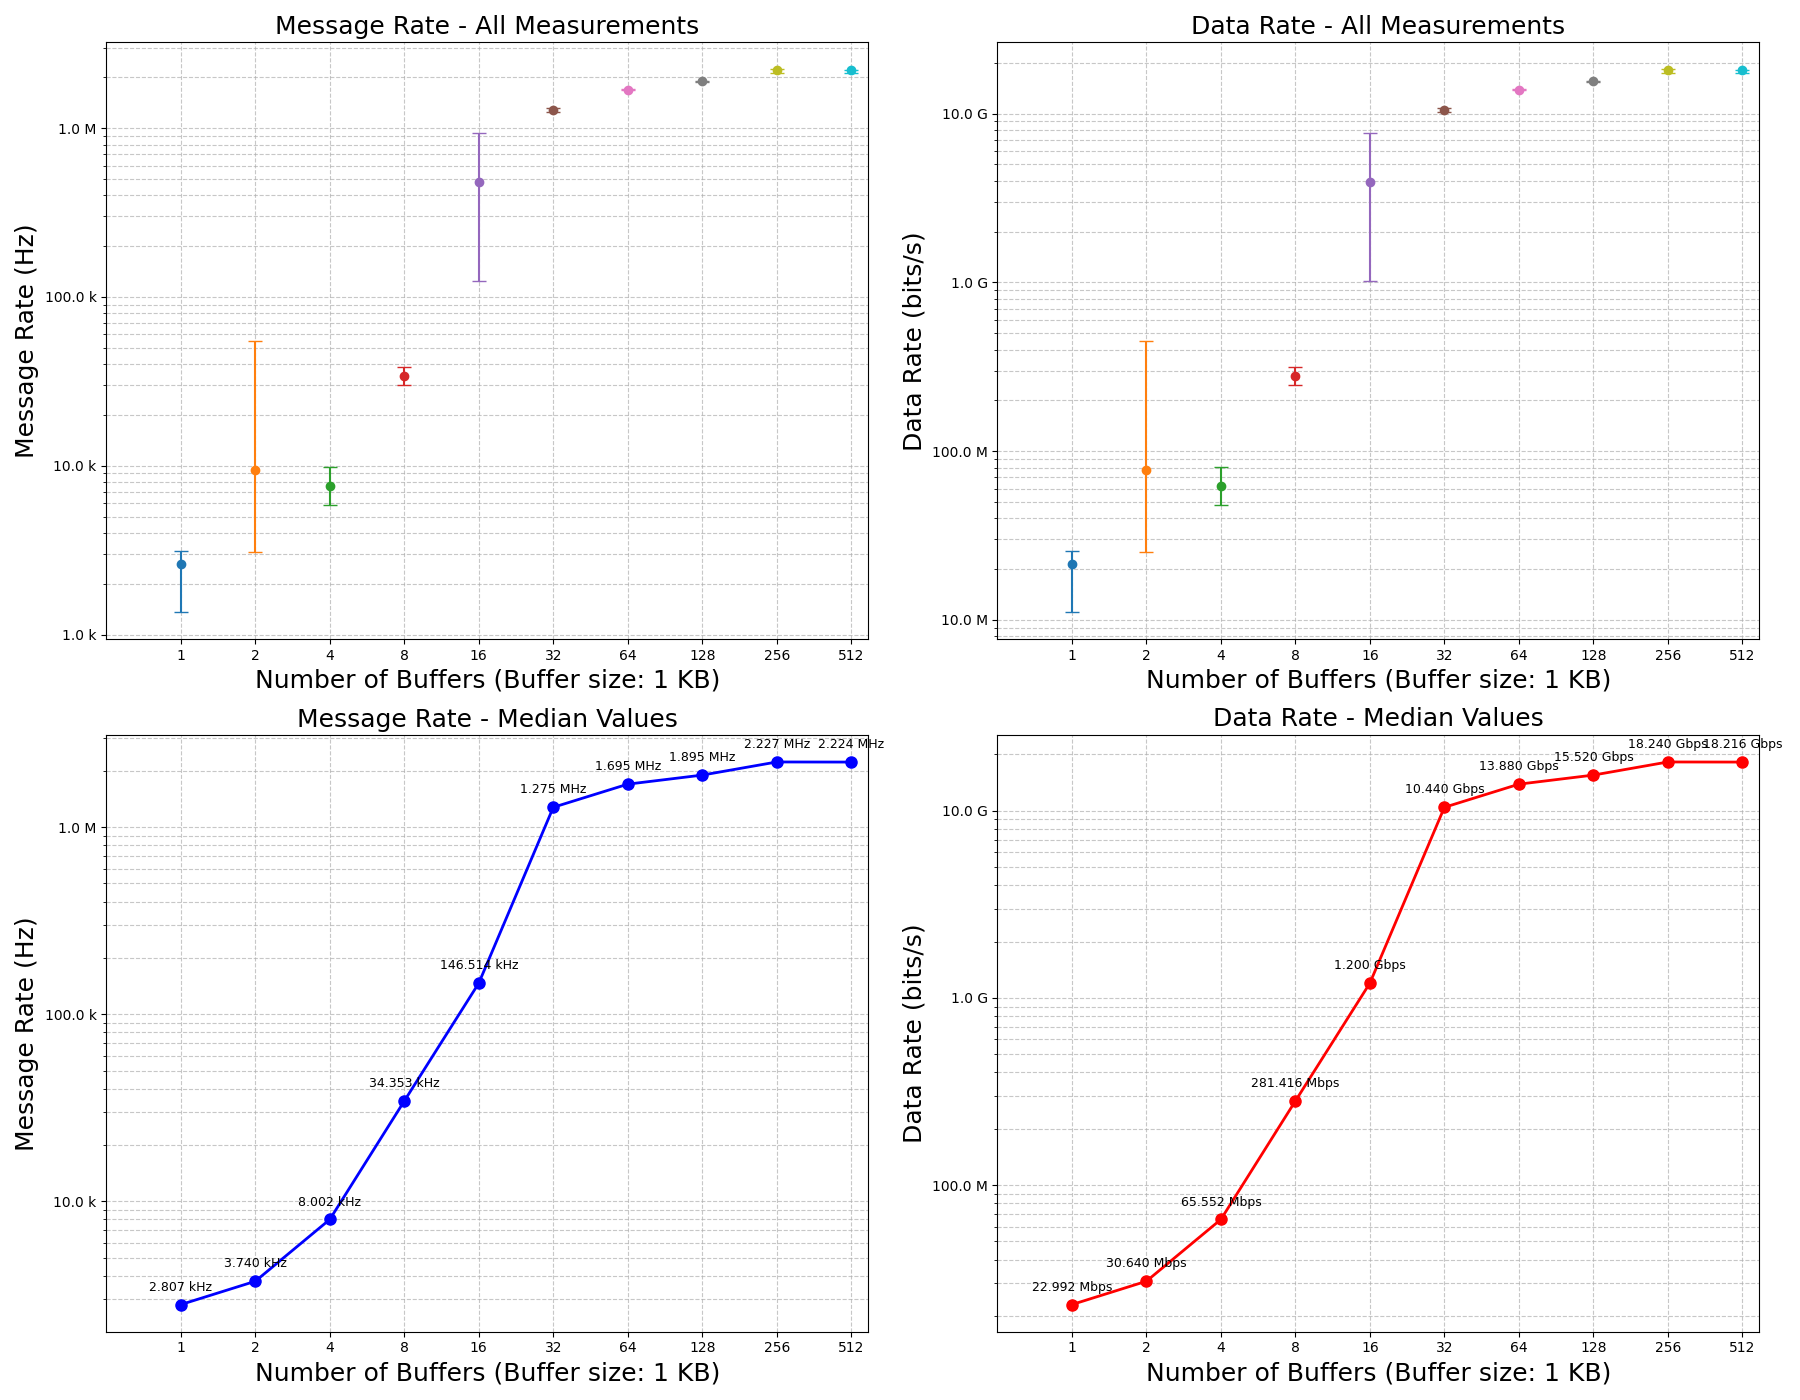
\includegraphics[width=\textwidth]{images/results/libfabric_throughput_analysis_1K.png}
    \caption[Network performance with a 1 KB buffer]{Network performance with a 1 KB buffer. \textbf{Left:} message frequency, \textbf{Right:} Data Throughput. \textbf{Top:} plots with error ranges, \textbf{Bottom:} median values.}
    \label{fig:1kb-buffer-throughput}
\end{subfigure}
\vspace{0.2cm}
\begin{subfigure}[b]{0.7\textwidth}
    \centering
    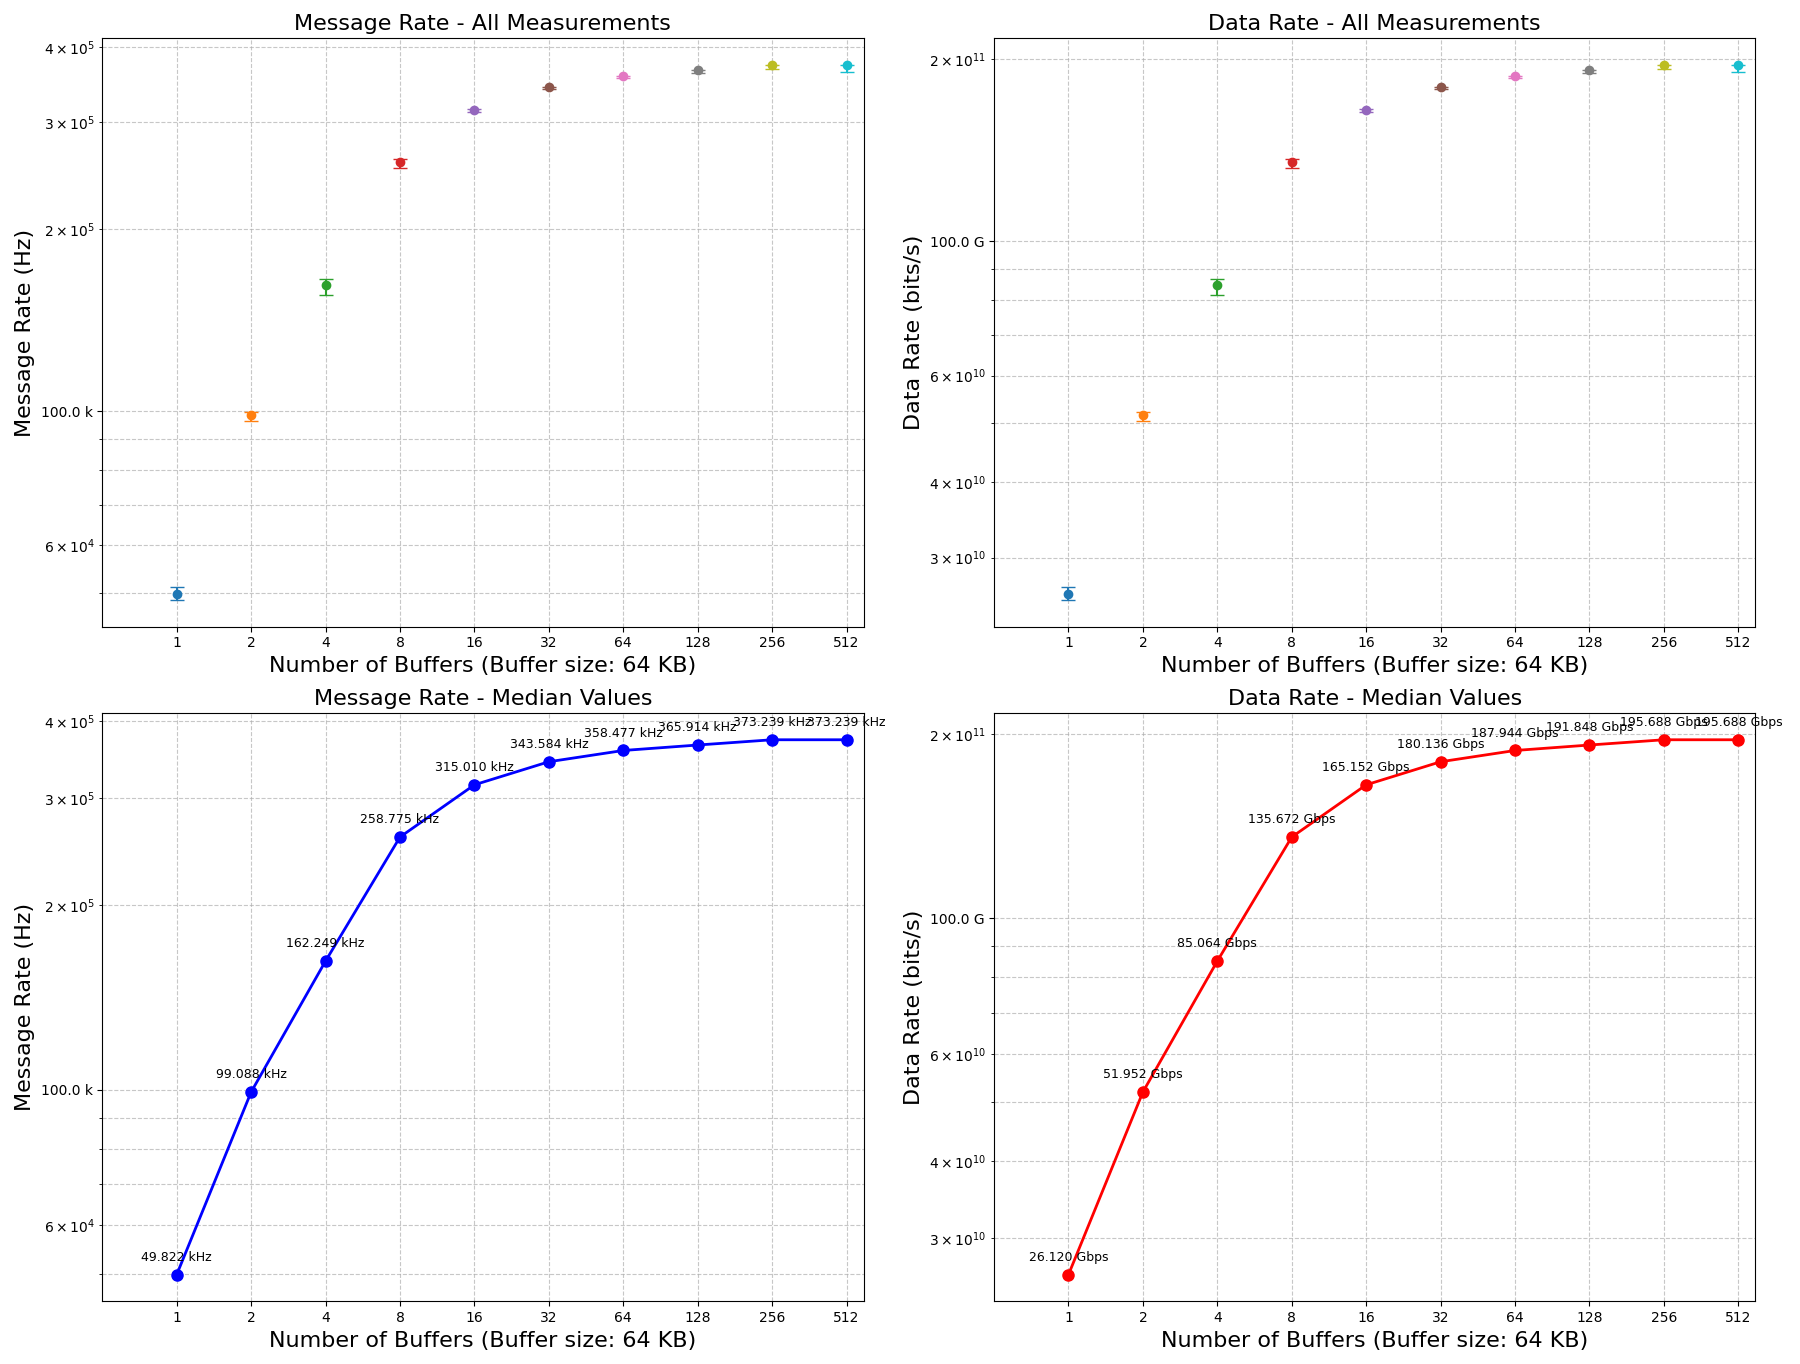
\includegraphics[width=\textwidth]{images/results/libfabric_throughput_analysis_64K.png}
    \caption[Network performance with a 64 KB buffer]{Network performance with a 64 KB buffer. \textbf{Left:} message frequency, \textbf{Right:} Data Throughput. \textbf{Top:} plots with error ranges, \textbf{Bottom:} median values.}
    \label{fig:64kb-buffer-throughput}
\end{subfigure}
\caption[Throughput comparison of 1KB and 64KB buffer]{The error rate of the smaller 1KB buffers is relatively high, while for the 64KB buffers the effect is much more contained.}
\label{fig:throughput-of-the-extremes-1K-64K}
\end{figure}

The results indicate that smaller buffers (e.g., 1 KB) exhibit higher error rates due to the overhead associated with connection establishment, which is significant relative to the transmission time for small messages. In contrast, larger buffers (e.g., 64 KB) exhibit a small variance, as the connection overhead becomes negligible compared to the transmission time.

To mitigate the impact of these variations (especially for smaller buffers), the median throughput was used for comparison.

Figure \ref{fig:libfabric-mean-throughput-comparison} presents the throughput comparison for LIBFABRIC-RDMA across all buffer sizes. The results highlight that buffers smaller than 8 KB and a fewer number of buffers than 16 should be avoided. For larger buffers, the behavior aligns with expectations. 
An interesting observation can be made about smaller buffers achieving the expected rate.

\begin{figure}[htbp]
\centering
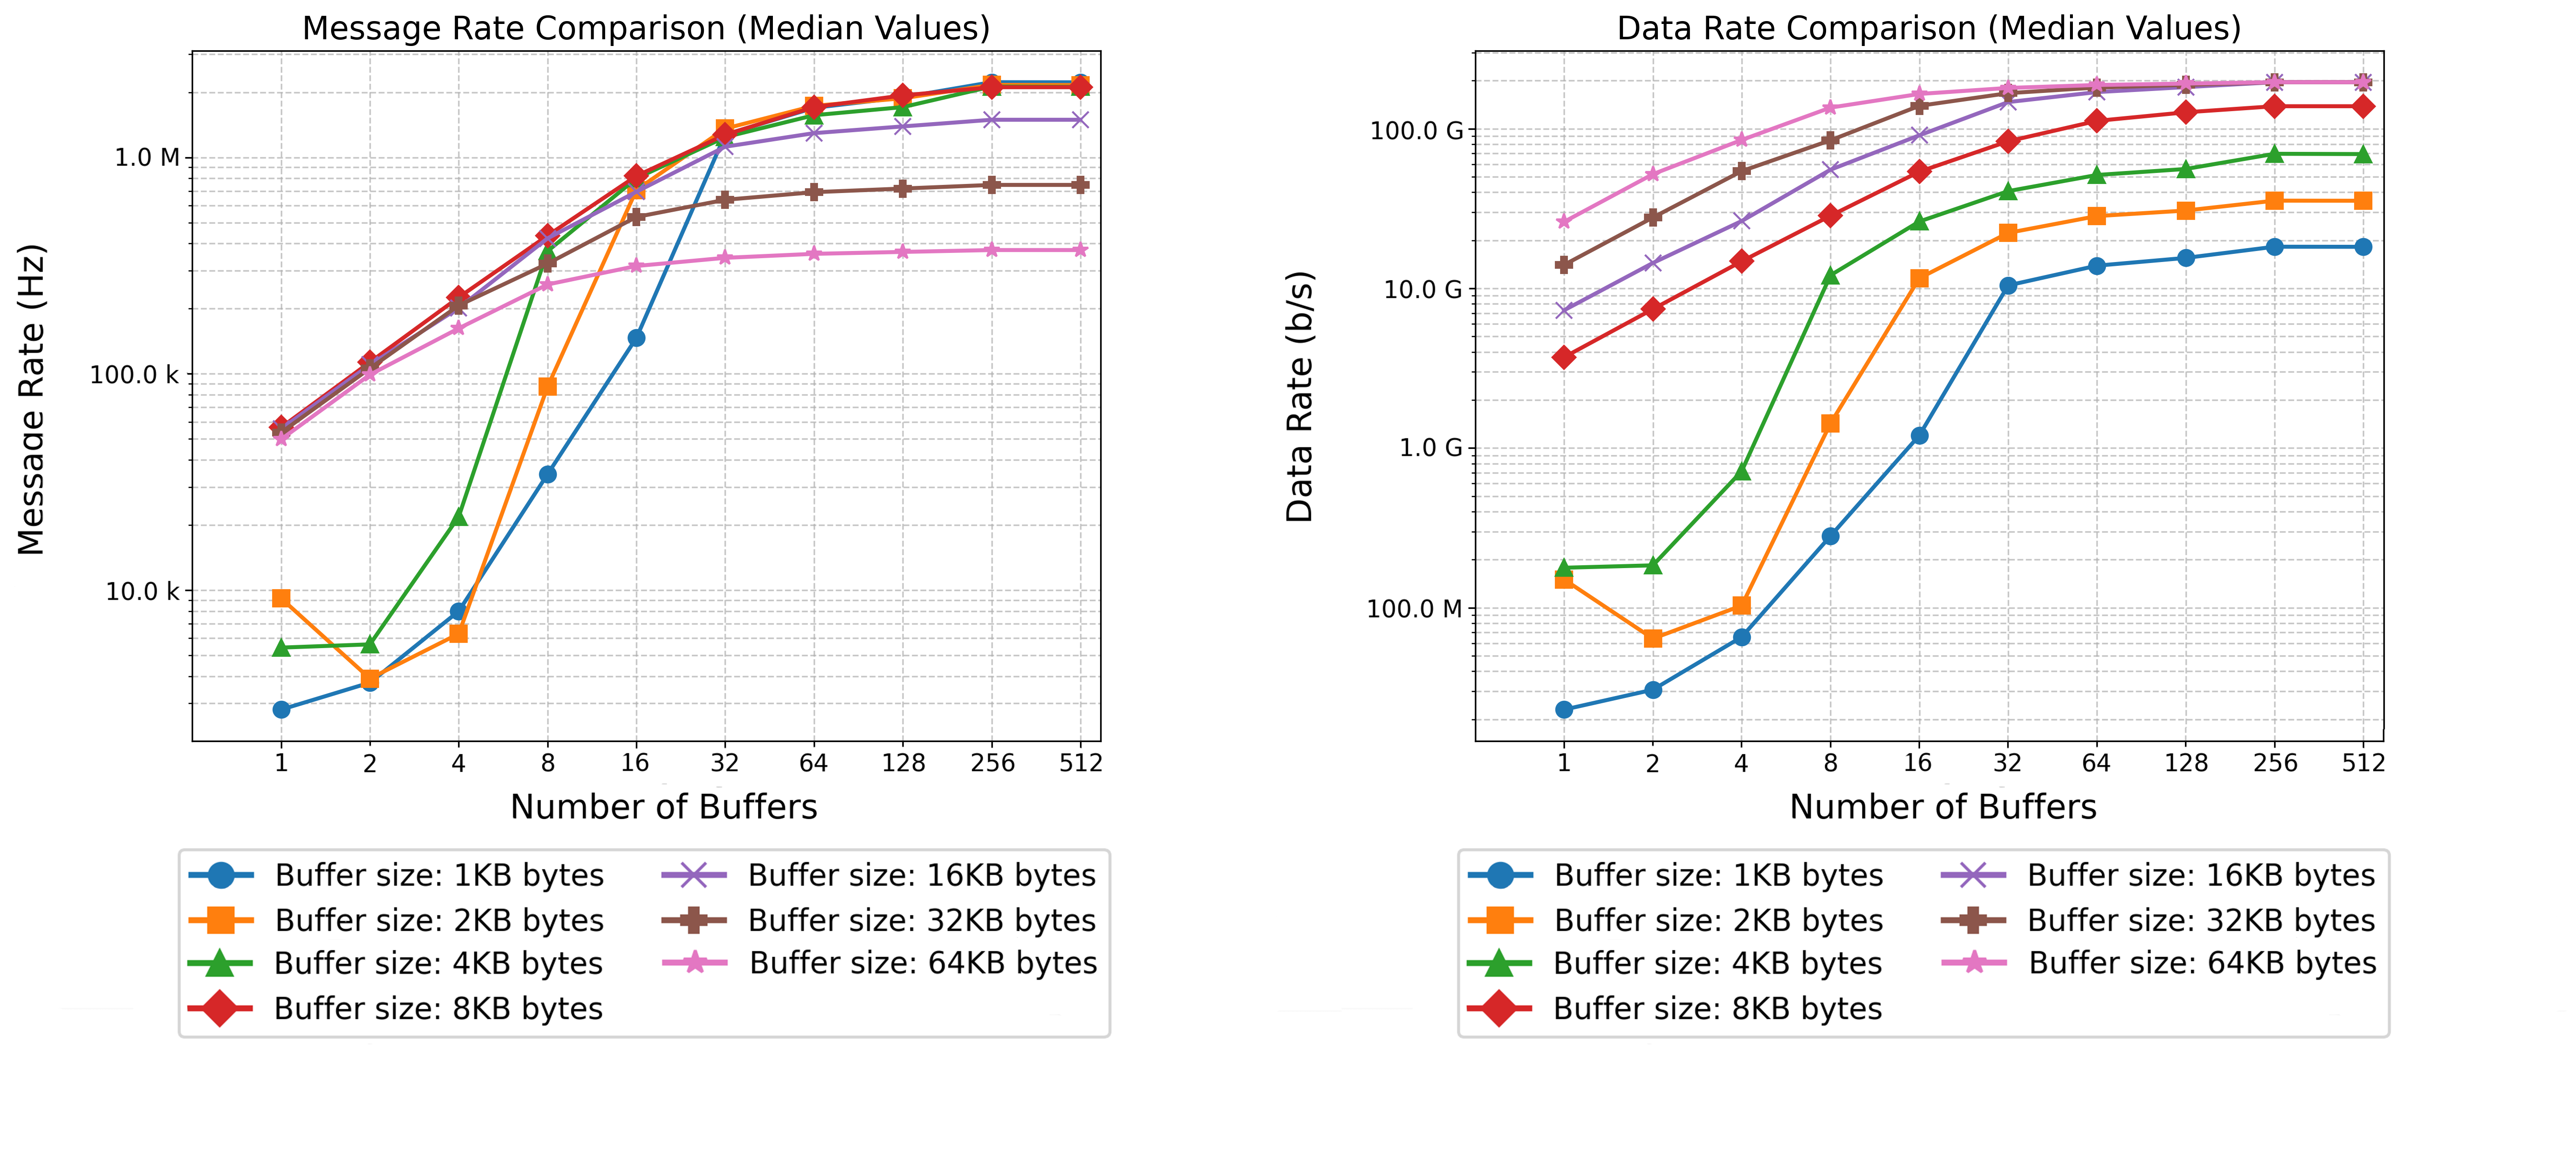
\includegraphics[width=\textwidth]{images/results/libfabric_performance_comparison.png}
\caption[Throughput comparison for LIBFABRIC-RDMA across all buffer sizes]{Throughput comparison for LIBFABRIC-RDMA across all buffer sizes. Left: frequency; Right: throughput.}
\label{fig:libfabric-mean-throughput-comparison}
\end{figure}

The throughput results also demonstrate that the 200 Gbps bandwidth is quickly saturated when using larger buffers. Notably, the network library can handle 64 KB buffers at 100 MHz, meeting the requirements for Phase II production.

For ASYNCMSG-TCP, the results (Figure \ref{fig:tcp-mean-throughput-comparison}) reveal that smaller buffers consistently achieve higher rates, regardless of the number of buffers. The throughput is significantly lower than LIBFABRIC-RDMA, with rates ranging from 70 to 90 kHz and a maximum throughput below 10 Gbps. This performance disparity shows once again that LIBFABRIC-RDMA can handle larger amount of data compared to ASYNCMSG-TCP.

\begin{figure}[htbp]
\centering
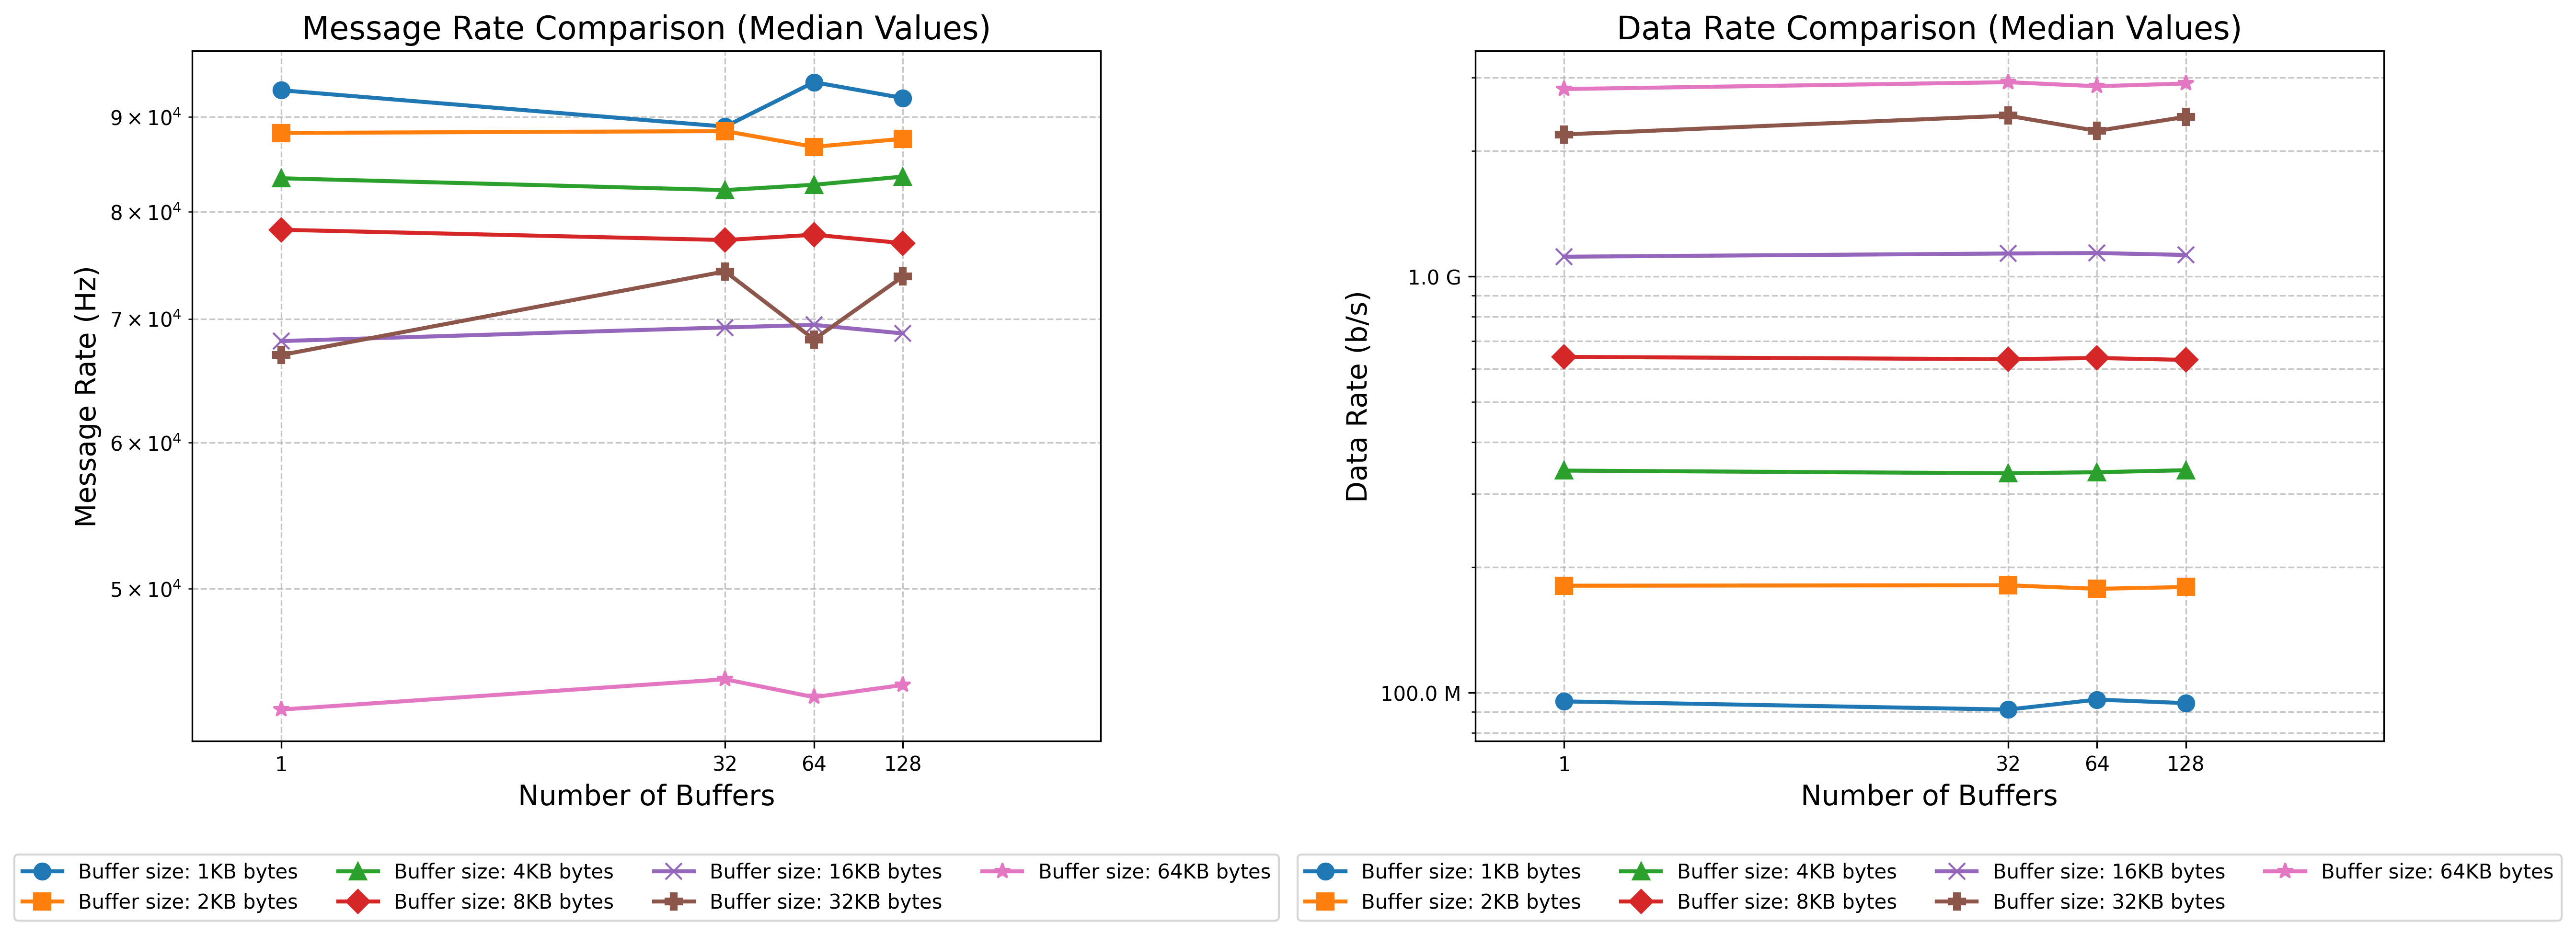
\includegraphics[width=\textwidth]{images/results/tcp_performance_comparison.png}
\caption[Throughput comparison for ASYNCMSG-TCP across all buffer sizes]{Throughput comparison for ASYNCMSG-TCP across all buffer sizes. Left: frequency; Right: throughput.}
\label{fig:tcp-mean-throughput-comparison}
\end{figure}

The decision to limit the number of buffers and sizes tested for ASYNCMSG-TCP was based on the observed saturation of bandwidth for LIBFABRIC-RDMA and the lack of performance improvement for ASYNCMSG-TCP with larger buffers. These findings conclusively demonstrate that LIBFABRIC-RDMA outperforms ASYNCMSG-TCP in terms of data throughput.

Given those results, why is TCP included as an option? One of the reasons is that it is less computationally demanding than \acs{RDMA}, so it is a better choice where the computing power is limited (L1 Calorimeter for example). The other reason derives from internal needs of \acs{ATLAS} and how its monitoring works. In order to monitor the entirety of \acs{ATLAS}' \acl{FE} electronics many elinks need to be used, in that case using LIBFABRIC-RDMA would require creating a \acs{DMA} buffer for each of them, plus sometimes the network library is used to send configurations to \acs{FE} electronics, meaning that the buffers need to be big enough for such scenarios. It comes by itself that the amount of memory needed is very large, and that memory would not be used efficiently, also the use case of the monitoring does not require high performance, thus ASYNCMSG-TCP is ideal.

\clearpage
\section{Performance measurements: felix-tohost}

\texttt{felix-tohost} represents the data direction from the Detectors to the T-DAQ infrastructure and between. The measurements that follow were conducted on the same device and host used for the \texttt{netio3} performance evaluation (Section~\ref{sec:netio3-perf}). 
Figure~\ref{fig:tbed-setup} below illustrates the setup for the test.\\
\emph{pc-tbed-felix-15} mounts the currently used in production \emph{FLX-712} with the \emph{F-EMU} firmware, which is used to emulate data in the FULLMODE format; that data will be written inside \acs{DMA} buffers on the other machine through \acs{E-link}s. It can be configured which \acs{E-link} writes in which \acs{DMA} buffer using the \emph{elinkconfig} tool. In the context of this test, all the 12 links have been used, specifically 3 links per \acs{DMA} buffer. 
On the same machine runs \emph{felix-test-swrod}, which is a software that subscribes to the \acs{E-link}s through \texttt{felix-tohost}, which in turn publishes the data when available.
On \emph{pc-tbed-felix-14} is mounted an \emph{FLX-182-1B} card, which is a prototype for the Phase II upgrade, with FULLMODE firmware. On the machine runs \texttt{felix-tohost}, which, as mentioned, will publish the data received from the emulator to \emph{felix-test-swrod} and will post the monitoring data so that a Prometheus instance running on Docker on my local machine could scrape it, and in turn Grafana could query Prometheus for the data scraped and create the Dashboard seen in Figure~\ref{fig:tohost-perf}. On \emph{pc-tbed-felix-14}, there is also the \acl{TTC} emulator that gives the pace to the FULLMODE emulator; in this test, the emulator trigger signals were set at 1 MHz.\\
For what concerns the \emph{netio3} network library, LIBFABRIC-RDMA was used.\\
The test consisted of sending data through all 12 links distributed across 4 \acs{DMA} buffers (3 links per \acs{DMA} buffer) at a steady 1 MHz rate, but changing the \emph{chunk} size.\\
As a reminder, in FULL mode, each link is not subdivided into \acs{E-link}s.

\begin{figure}[htbp]
\centering
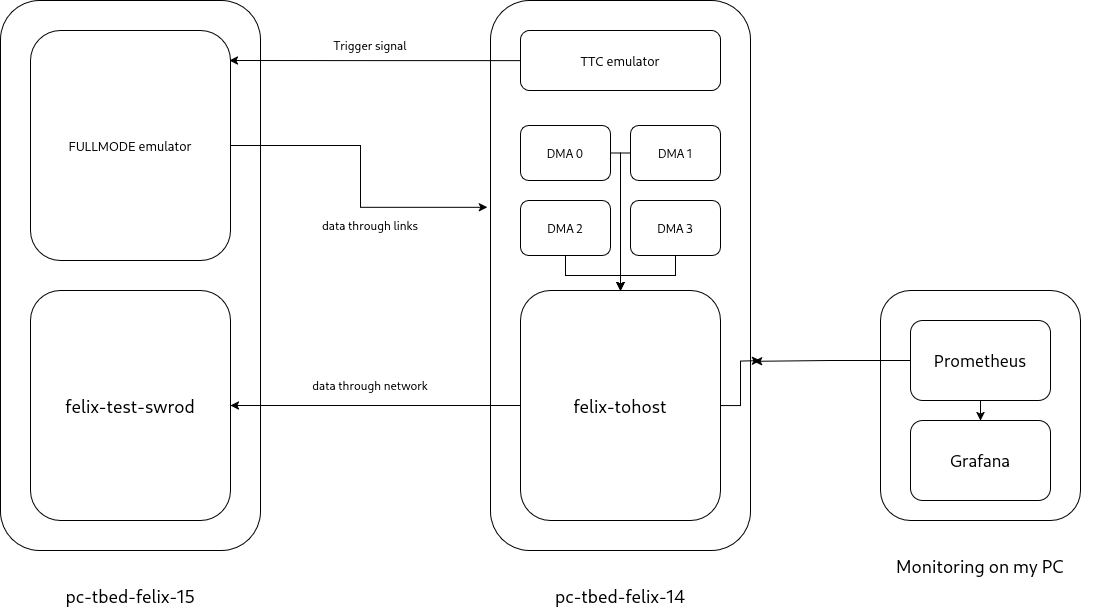
\includegraphics[width=\textwidth]{images/results/tohost-tbed-setup.png}
\caption[Testbed configuration]{Testbed configuration. F-EMU firmware is installed on the felix-15 machine, felix-tohost is running on the felix-14 machine which also sends the monitoring data to Prometheus.}
\label{fig:tbed-setup}
\end{figure}

The monitoring system described in Section~\ref{sec:felix_monitoring} was employed to record the performance evaluation, in particular the Prometheus-Grafana solution. The test was conducted by gradually increasing the \emph{chunk} size while maintaining a steady rate of 1 MHz (what is the requirement for Phase II). This behavior is illustrated in the dashboard window titled "Average Chunk Size" (Image~\ref{fig:tohost-perf}), where the average chunk size ramps, with incremental steps, from 16 bytes to 2 KB. Starting at a chunk size of 1 KB, by looking at the \emph{E-link Chunk Rate} graph it appears that performance issues begin to arise.\\
What in reality is shown in the image is not a performance issue, but it is the reach of the physiological limit of FULL mode. To recall, the Subsection~\ref{subsec:felix-fullmode} explains that FULL mode has a maximum theoretical throughput of about 7.68 Gbps per link (after encoding, which is our case), and in the graph it is shown that the \acs{DMA} buffers are not getting filled up (\emph{Free Space in DMA Buffer} graph), there is no backpressure in the network (\emph{Network Resources} graph) and the chunks are not being truncated (\emph{Chunks Truncated} graphs). at a rate of 1MHz, sending 1KB of data per chunk means that the throughput is about 8.2 Gbps, and at 2KB it is about 16.4 Gbps, which is above the maximum throughput of the link, thus the link chunk rate diminishes untill reaching 7.68 Gbps throughput.\\ 
To recap, in figure~\ref{fig:tohost-perf} is shown that \texttt{felix-tohost} and the card \texttt{FLX-182-1B} can handle without signs of distress data rates that reach the technological limit of FULL mode.

\begin{figure}[htbp]
\centering
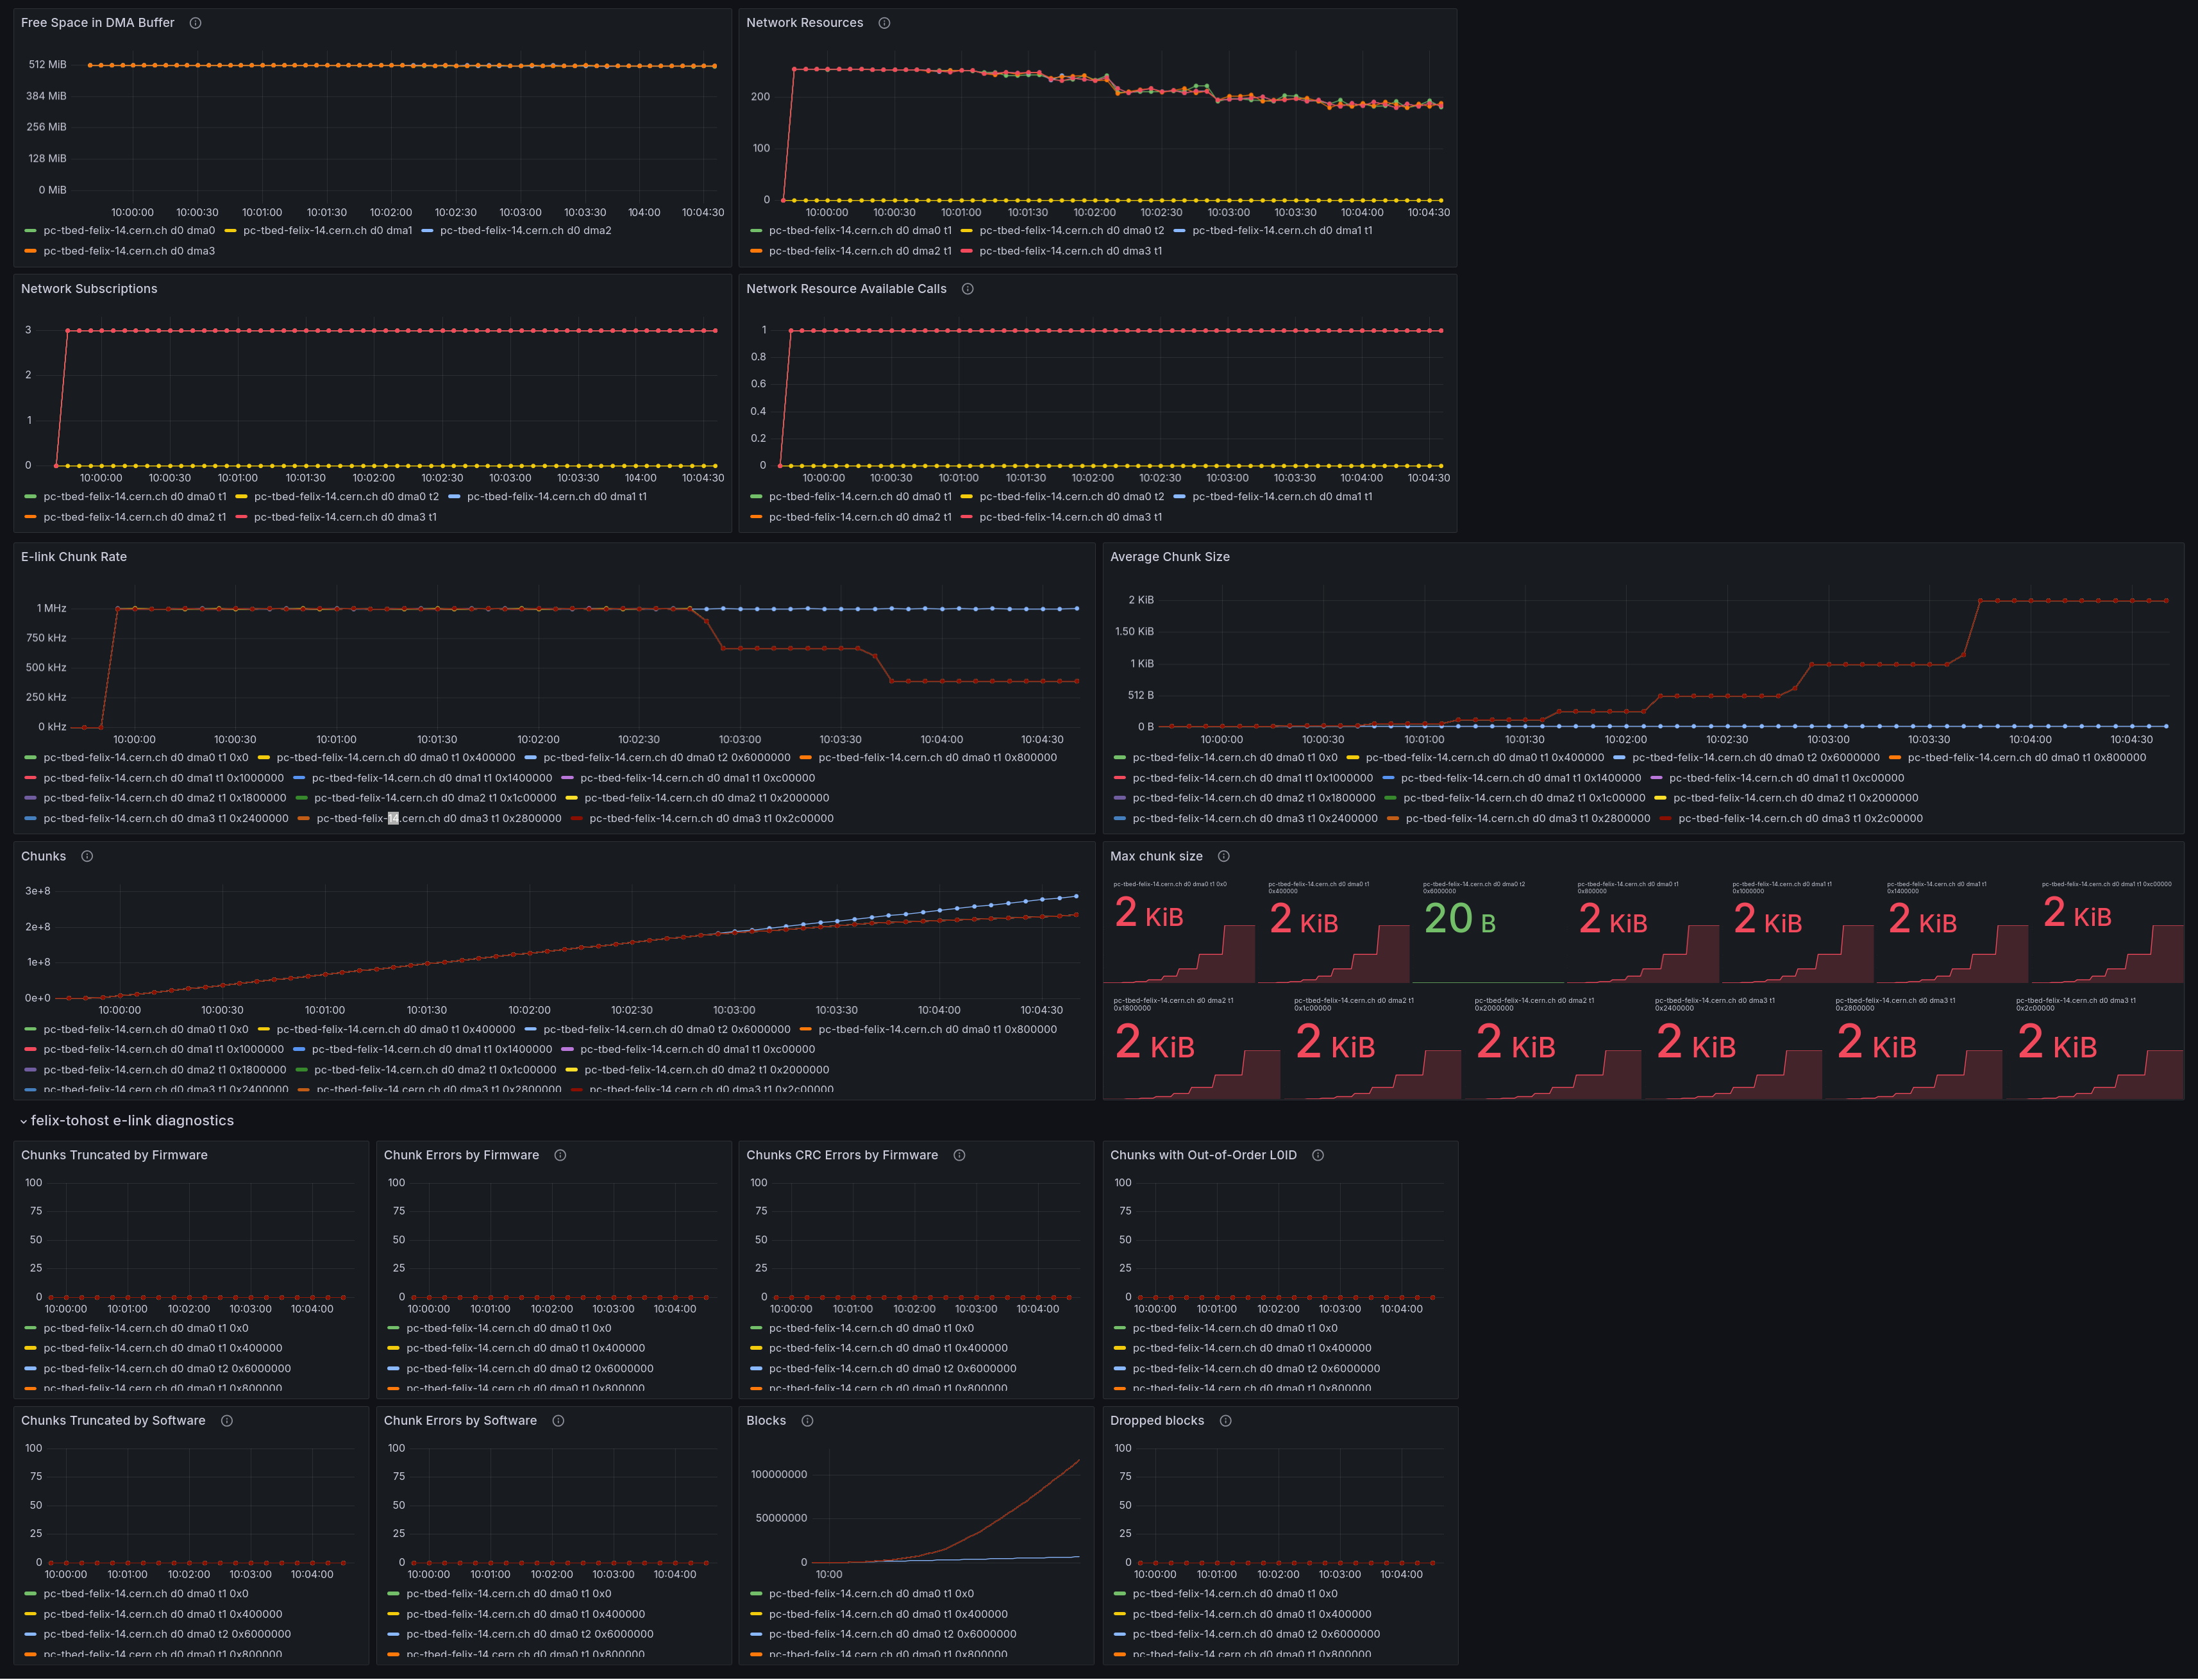
\includegraphics[width=\textwidth]{images/results/tohost-perf.png}
\caption{Grafana monitoring: stress test at 1 MHz rate up to 2 KB chunks.}
\label{fig:tohost-perf}
\end{figure}

Figure~\ref{fig:cpu-usage} illustrates the CPU usage per chunk size. The percentage value represents the average CPU usage over a 30-second period. Given that the host machine has 64 CPU cores, the results demonstrate that \emph{felix-tohost} is not very resource-intensive.

\begin{figure}[htbp]
\centering
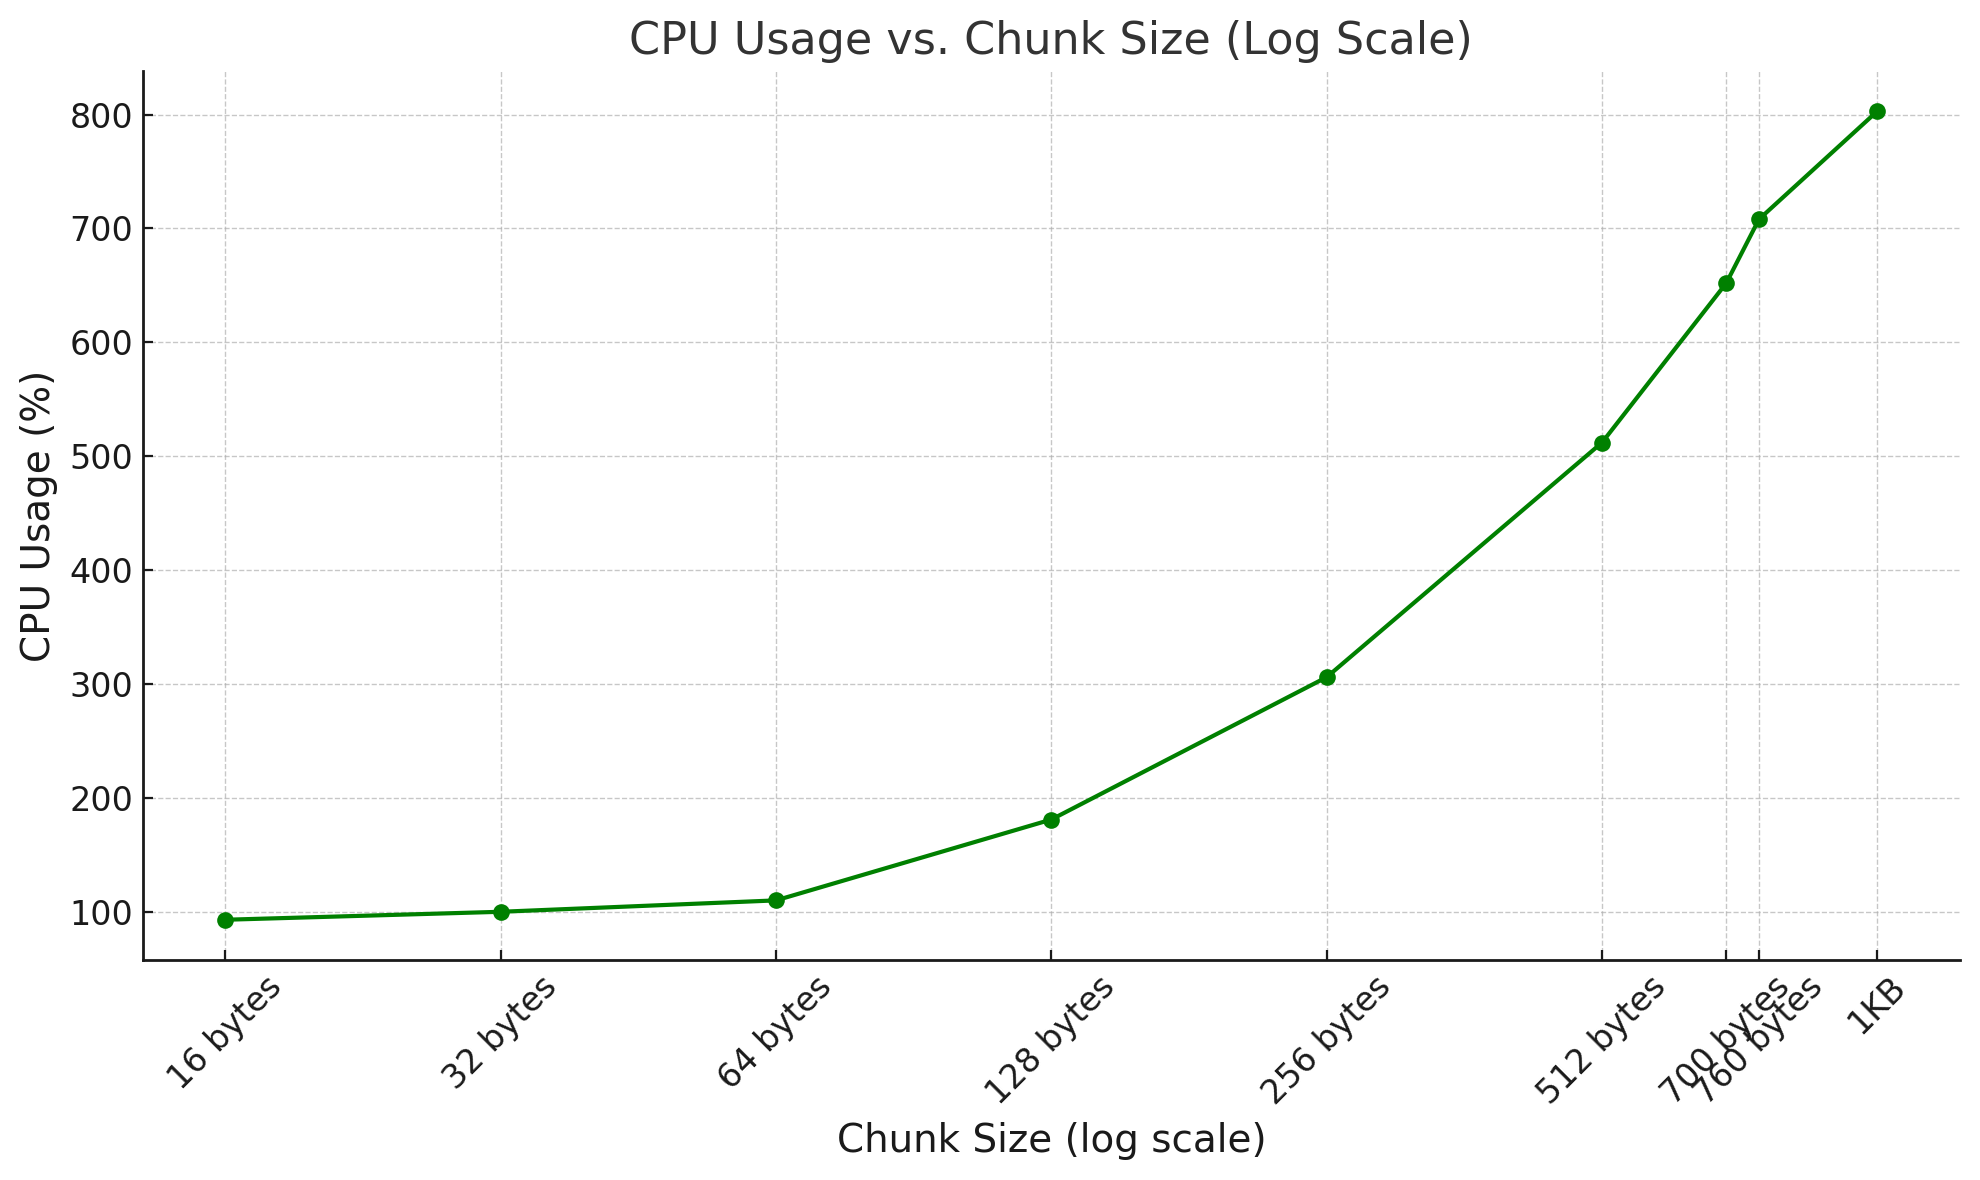
\includegraphics[width=\textwidth]{images/results/cpu-usage-chunk-size-1MHz.png}
\caption[CPU usage per chunk size at 1 MHz]{CPU usage per chunk size at 1 MHz. 100\% corresponds to one physical CPU core.}
\label{fig:cpu-usage}
\end{figure}

The execution of \texttt{felix-tohost} was analyzed using \texttt{perf}, and from the output a FlameGraph \cite{flamegraph} was generated (Figure~\ref{fig:felix-tohost-flamegraph}). The FlameGraph, an interactive \emph{svg} file viewable in a web browser, shows that a significant portion of the execution time is spent on functions such as \emph{decode\_subchunk\_headers}, \emph{post\_subchunk}, and \emph{check\_block\_integrity}, as well as chunk-copying operations. This flamegraph shows hotpost areas in the code that can potentially be optimized, serving as a starting point for future developments (see Subsection~\ref{subsec:felix-tohost-improvement}).

\begin{figure}[htbp]
\centering
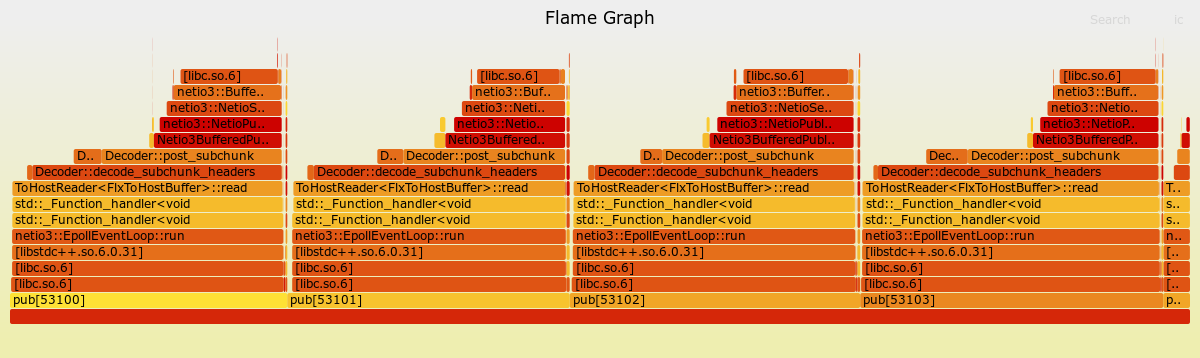
\includegraphics[width=\textwidth]{images/results/flamegraph.png}
\caption[Flamegraph of felix-tohost]{Flamegraph of \texttt{felix-tohost}. It highlights four main processes, each corresponding to one \acs{DMA} buffer, along with a smaller fifth process dedicated to \acs{TTC}.}\label{fig:felix-tohost-flamegraph}
\end{figure}
\chapter{Conclusions}

\section{Summary}
This thesis has addressed the challenges posed by the \acl{HL-LHC} era at \acs{CERN} with a focus on the \acs{FELIX} readout system. The thesis has introduced the \acs{FELIX} project and has presented the contributions to the open-source software \texttt{felix-distribution}, the network library \texttt{netio3}, and the hardware testing and benchmarking of the FLX-182-1B cards. This work has demonstrated that the throughput and scalability demands are being met. The benchmarks have validated the proposed solutions, confirming their suitability for future deployment in large-scale \acs{HEP} experiments. The \acs{FELIX} project is being noted and taken under consideration by the other large experiments at \acs{CERN} thanks to the collaboration and work of all the people involved.

\paragraph{\acs{FELIX} in other experiments}
\begin{itemize}
    \item \textbf{ProtoDUNE SP} \cite{protodune} is an experiment at \acs{CERN} whose purpose is to test and validate the technologies and design that will be applied to the construction of the \acs{DUNE} Far Detector at the Sanford Underground Research Facility. \acs{FELIX} is used for the readout.

    \item \textbf{NA62} \cite{protodune, Martellotti:2056863} is an experiment at \acs{CERN} that studies kaon decays. The \acs{FELIX} platform is used for data buffering, clock distribution and synchronous communication for control and configuration.

    \item \textbf{sPHENIX} \cite{sphenix} is an experiment located at \acl{BNL}, Long Island (New York), whose purpose is to learn about Quark-Gluon Plasma. \acs{FELIX} is used for the readout of three subdetectors.

    \item \textbf{SPIDR4} \cite{spidr4} is a readout system firmware, developed at Nikhef, that uses \acs{FELIX} as a readout system for Timepix4 \cite{timepix4}, a pixel based subdetector. 
\end{itemize}

\section{Future developments}

\subsubsection{felix-tohost improvement}
\label{subsec:felix-tohost-improvement}

In the analysis made with \emph{perf} on \texttt{felix-tohost}, with the FlameGraph results shown in Figure~\ref{fig:felix-tohost-flamegraph}, it is shown that the bottleneck is in decoding \emph{chunks} and \emph{subchunks} from the \emph{blocks} and in the copy operations. An improvement can be made by sending blocks directly instead of decoding them into chunks and then sending a netio3 encoded buffer.\\
Preliminary tests show that \texttt{felix-tohost} performance improves by a factor of 8 (800\%) in the case of 20-byte messages, without much burden on the client side. Further studies are needed to account for all possibilities, for example for chunks that are bigger than a 1KB block and what impact that would have on the performance on both server and client applications.

\subsubsection{cmem\_rcc replacement}

cmem\_rcc has been a very valid option during the years, but the reason it exists is because the Linux kernel could not offer a valid alternative. The last feasibility study is from 2018, when AlmaLinux (The official \acs{CERN} OS) used kernel 3.X, and the kernel 4.X was actively being developed. With kernel 6.X, \acs{DMA} and \acs{NUMA} support for it will be the default, making it an interesting option to avoid using custom kernel modules. At the moment (2025) AlmaLinux 9 is the official release, and it uses kernel 5.X. This replacement can be done only when AlmaLinux 10 with kernel 6.X is released, and supposedly it will happen in time to test the entire system before Phase II.

\subsubsection{Alternative architecture}

It is being taken into consideration to replace the current architecture with one that removes the networking between the \acs{FE} electronics and the data handler. This will reduce the flexibility of the architecture but is counterbalanced with many positive effects like cost savings, space savings, computing power, and energy consumption. In this architecture, the \acl{DH} software will be moved inside the \acs{FELIX} host server, which will need a more powerful CPU to sustain the newly added workloads, but this saves the cost of dedicated \acs{DH} servers. With this new arrangement, the \acs{DH} processes will read data directly from the \acs{FELIX} ToHost \acs{DMA} buffers. This requires software development to allow the data handler to use \acs{RDMA}.

\subsubsection{Using servers with ARM processors}

In an effort to reduce energy consumption at \acs{CERN}, it is being investigated whether ARM processors could be a valid alternative to x86 ones. It will require software adjustments, in particular in the \acs{FELIX} card driver side and kernel compilation.

\appendix
\chapter{UML Diagrams}
\label{ch:appendix}

\begin{sidewaysfigure}[htbp]
    \makebox[\textwidth][c]{
        \scalebox{1}[-1]{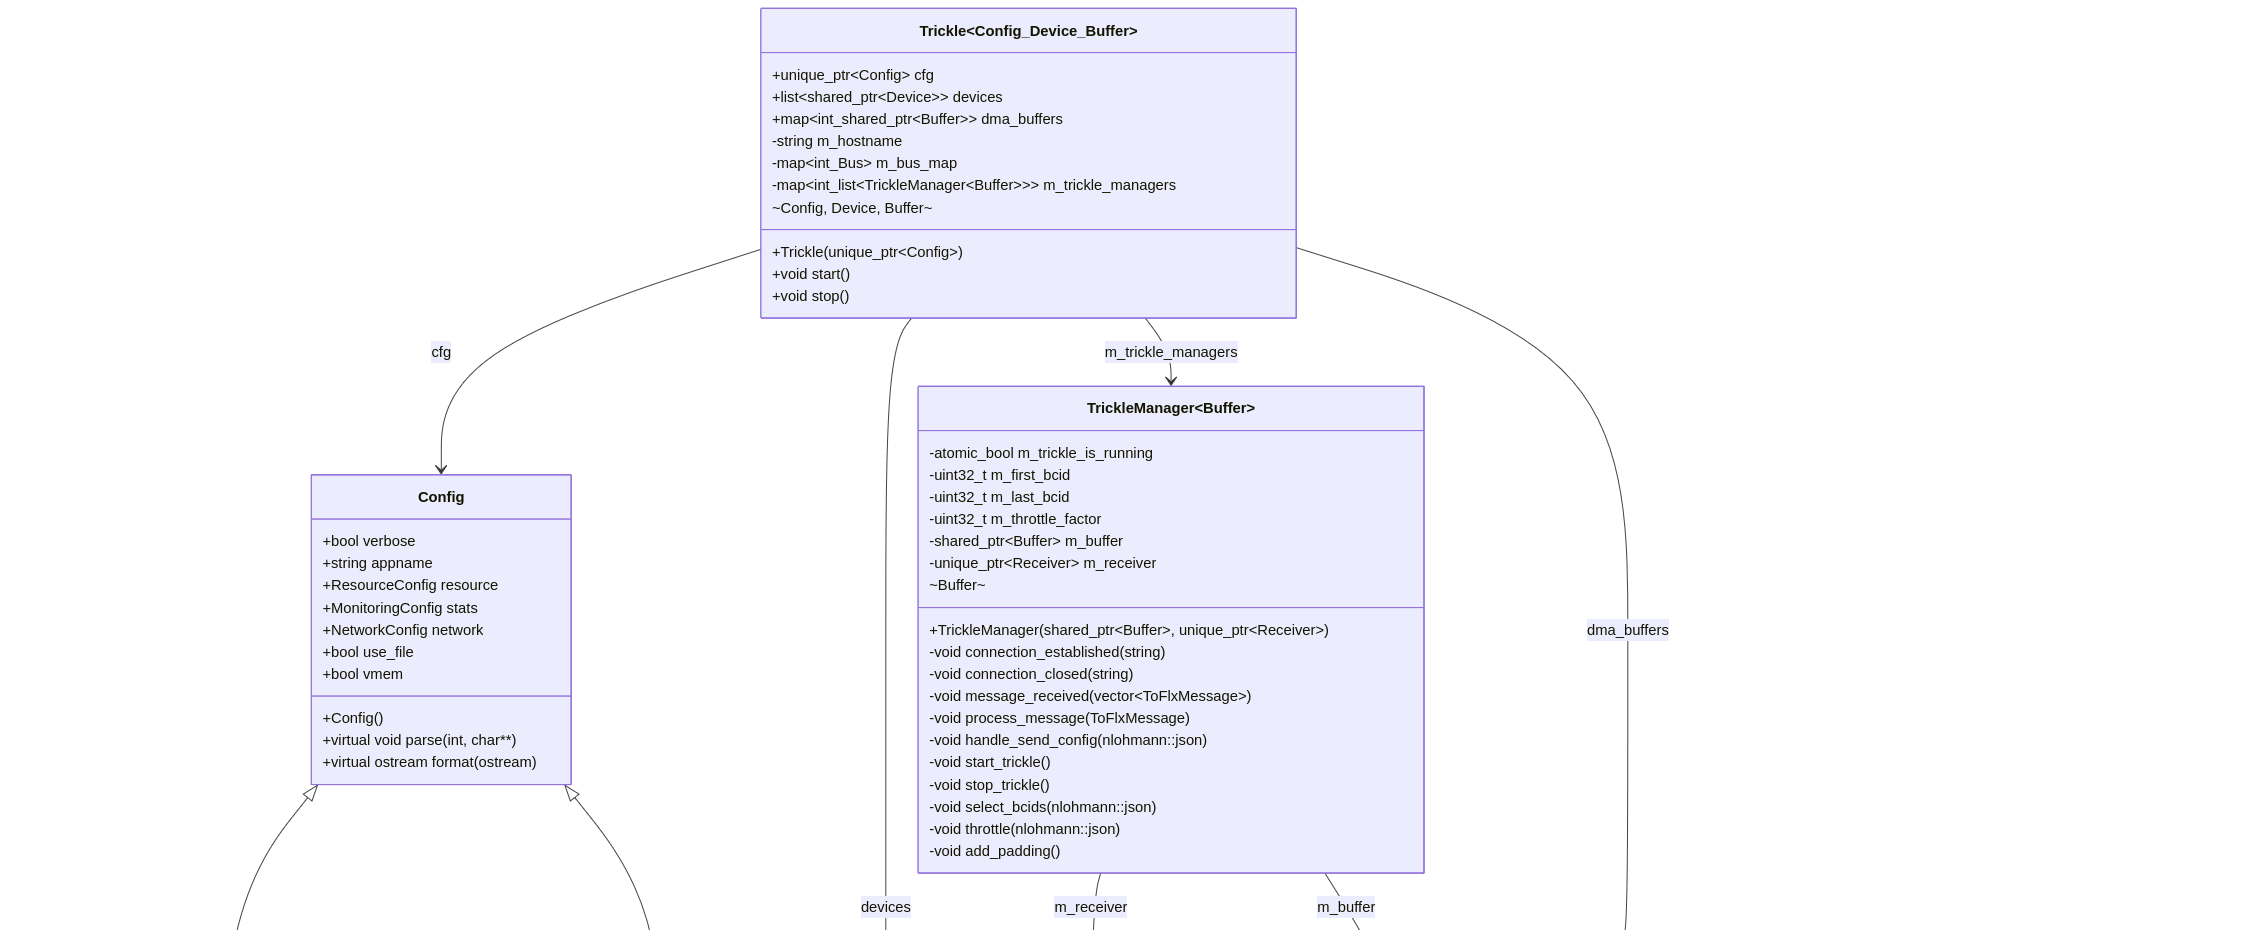
\includegraphics[width=1.2\textwidth]{images/appendix/complete-trickle-config-uml-top.png}}
    }
    \caption{Complete Trickle Configuration UML diagram. Top part (vertically mirrored)}
    \label{fig:complete-trickle-uml-top}
\end{sidewaysfigure}

\begin{sidewaysfigure}[htbp]
    \makebox[\textwidth][c]{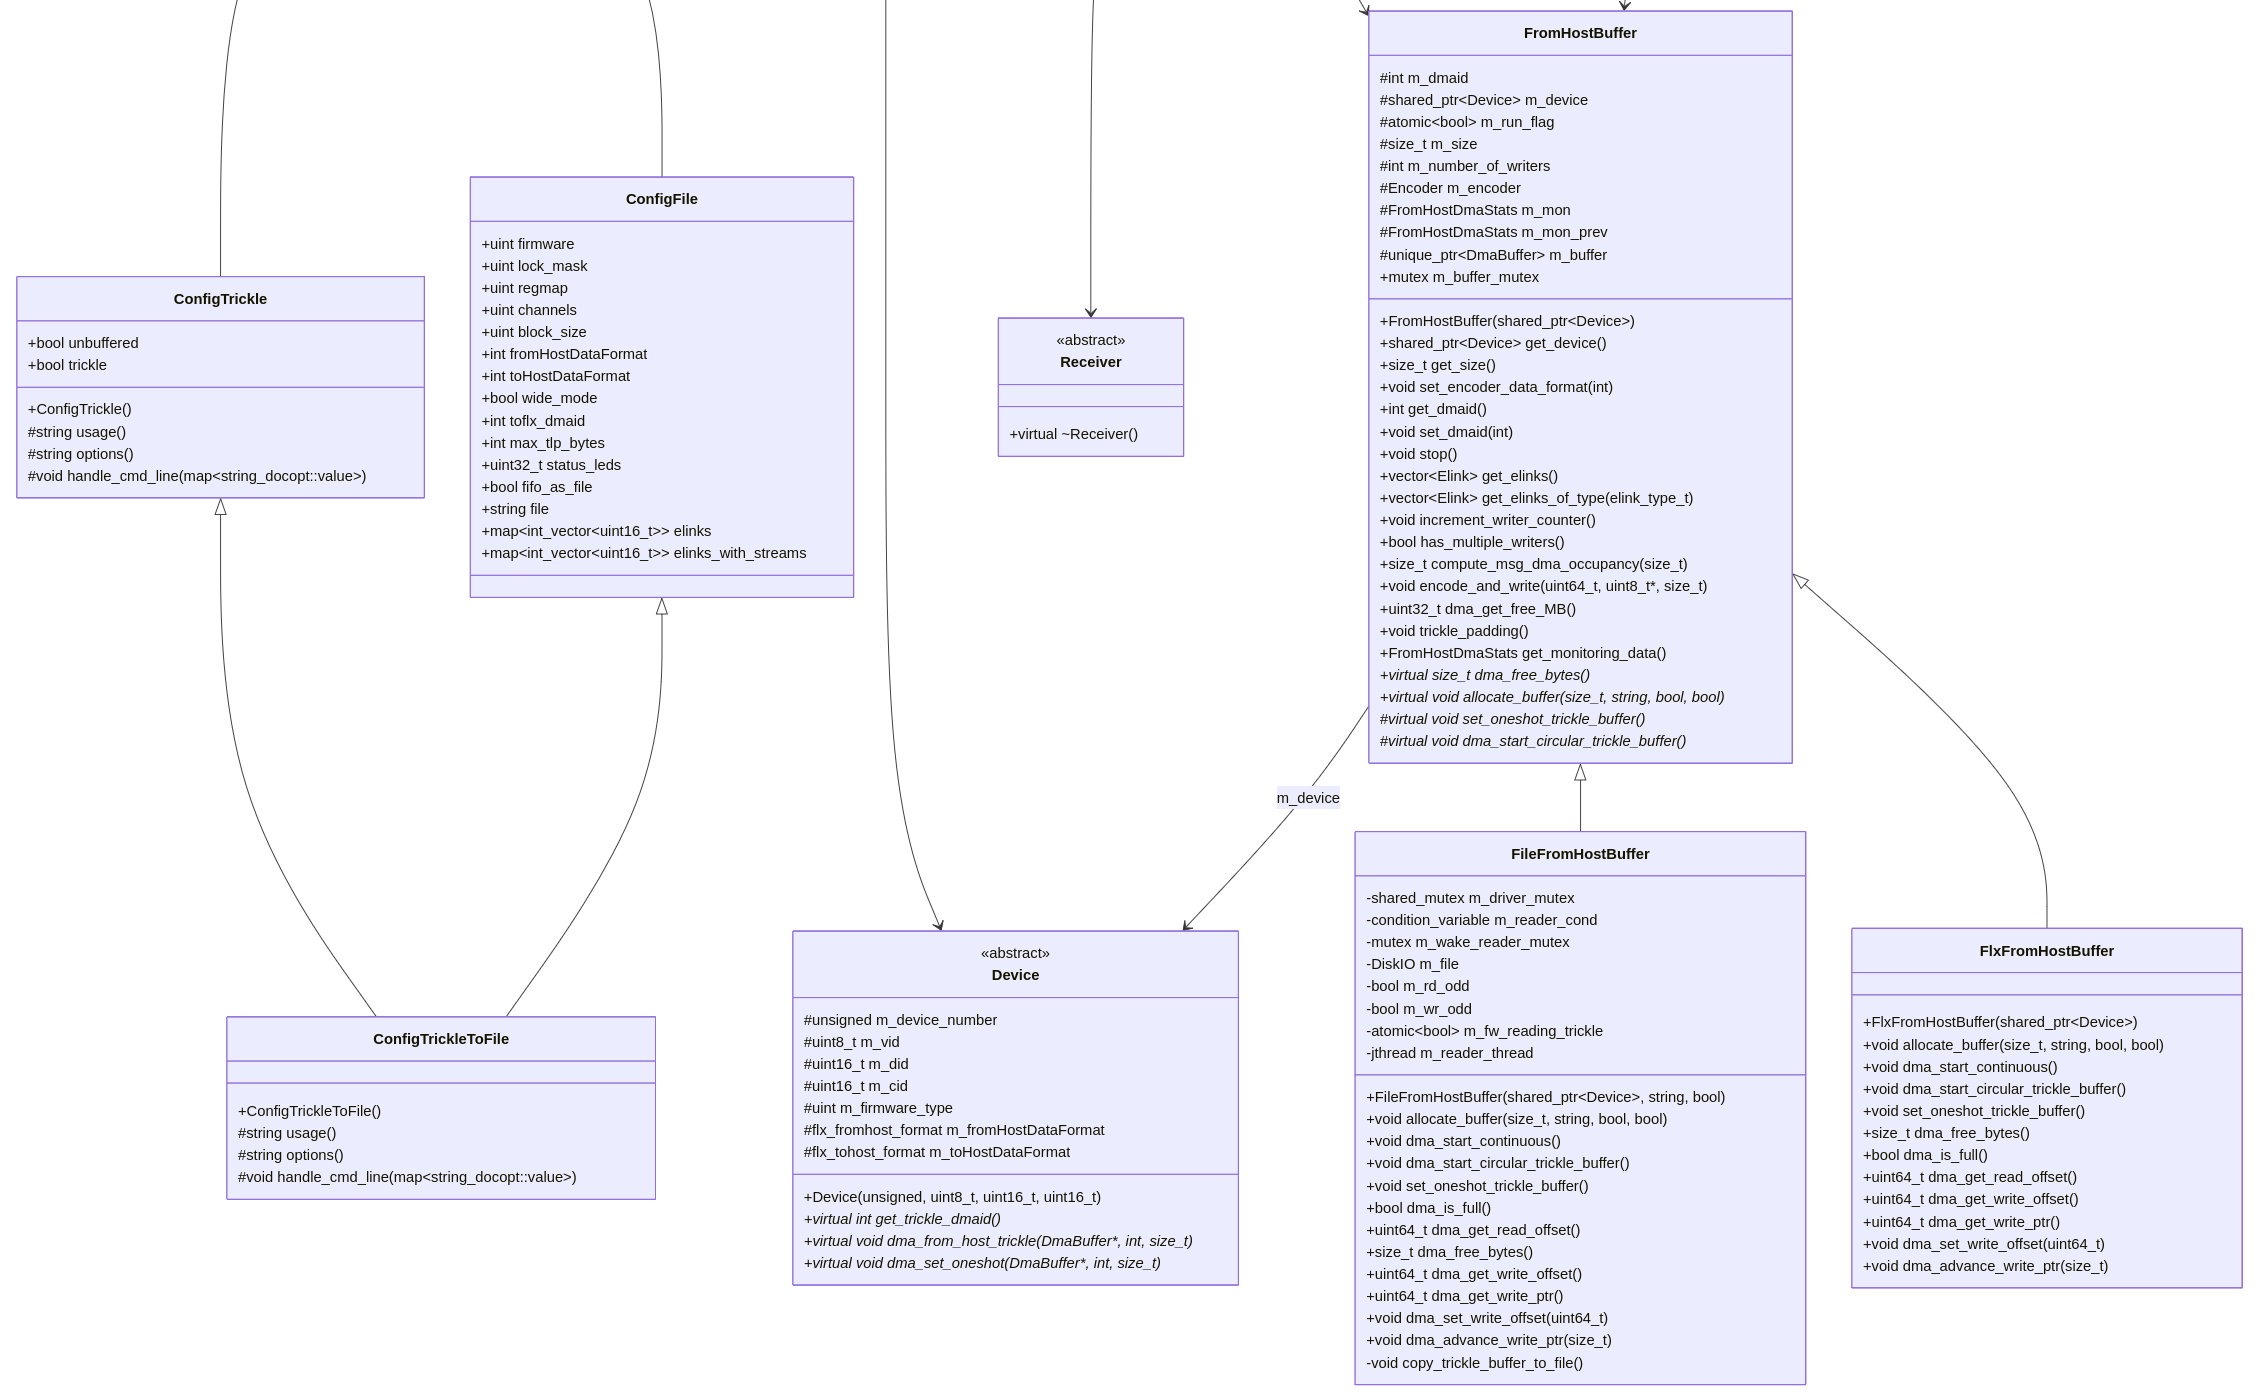
\includegraphics[width=1.2\textwidth]{images/appendix/complete-trickle-config-uml-bottom.png}}
    \caption{Complete Trickle Configuration UML diagram. Bottom part}
    \label{fig:complete-trickle-uml-bot}
\end{sidewaysfigure}

\clearpage

\begin{sidewaysfigure}
    \centering
    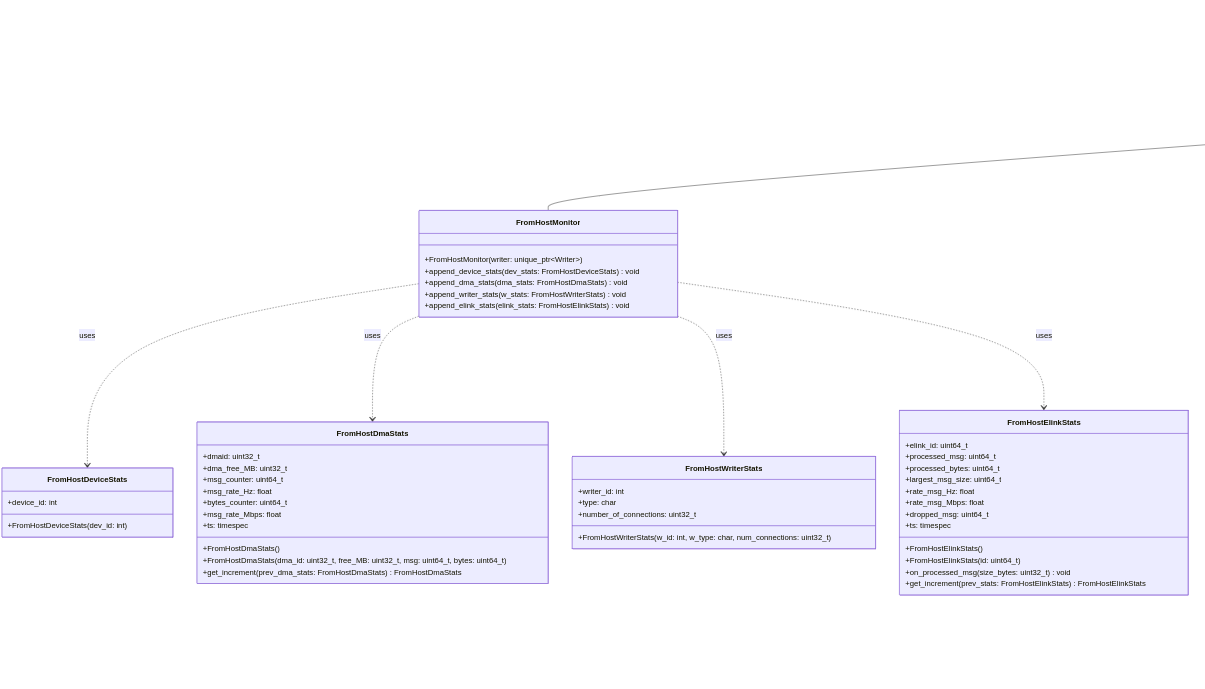
\includegraphics[width=\textwidth,height=\textheight,keepaspectratio]{images/appendix/complete-monitoring-uml-left.png}
    \caption{Complete Monitoring system UML diagram. Left part}
    \label{fig:complete-monitoring-uml-left}
\end{sidewaysfigure}

\begin{sidewaysfigure}
    \centering
    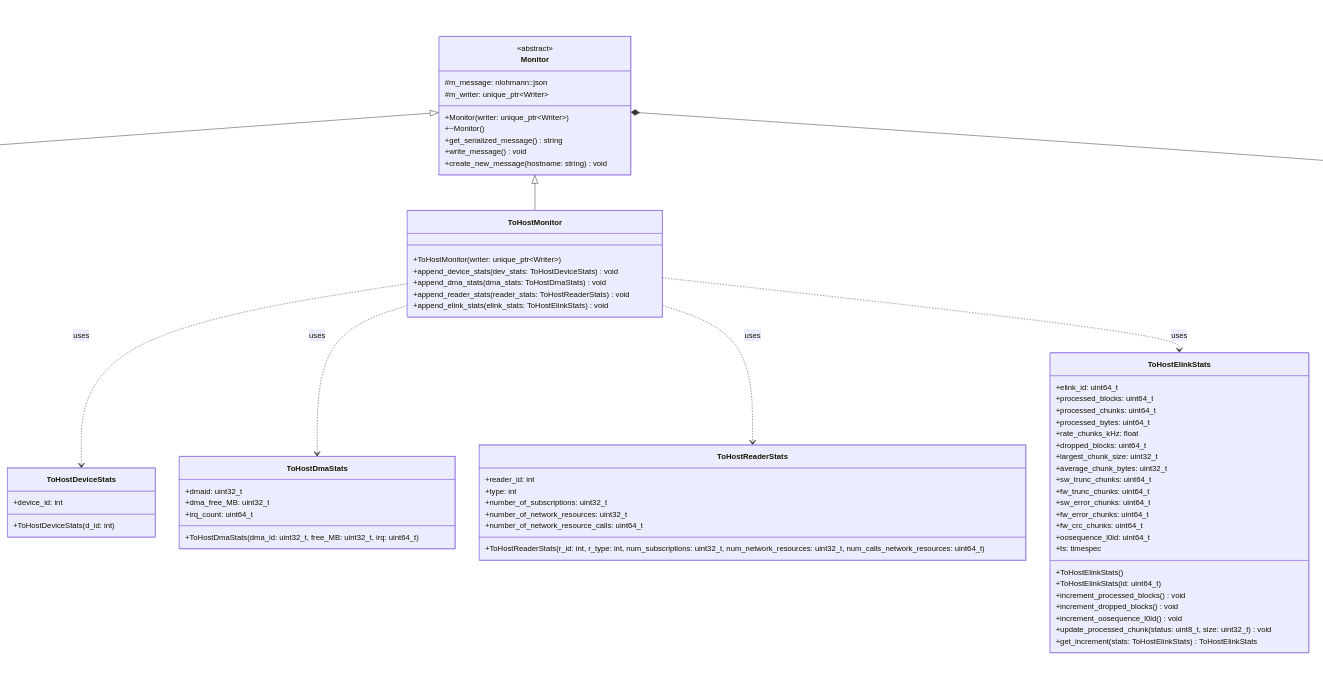
\includegraphics[width=\textwidth,height=\textheight,keepaspectratio]{images/appendix/complete-monitoring-uml-mid.png}
    \caption{Complete Monitoring system UML diagram. Middle part}
    \label{fig:complete-monitoring-uml-mid}
\end{sidewaysfigure}

\begin{sidewaysfigure}
    \centering
    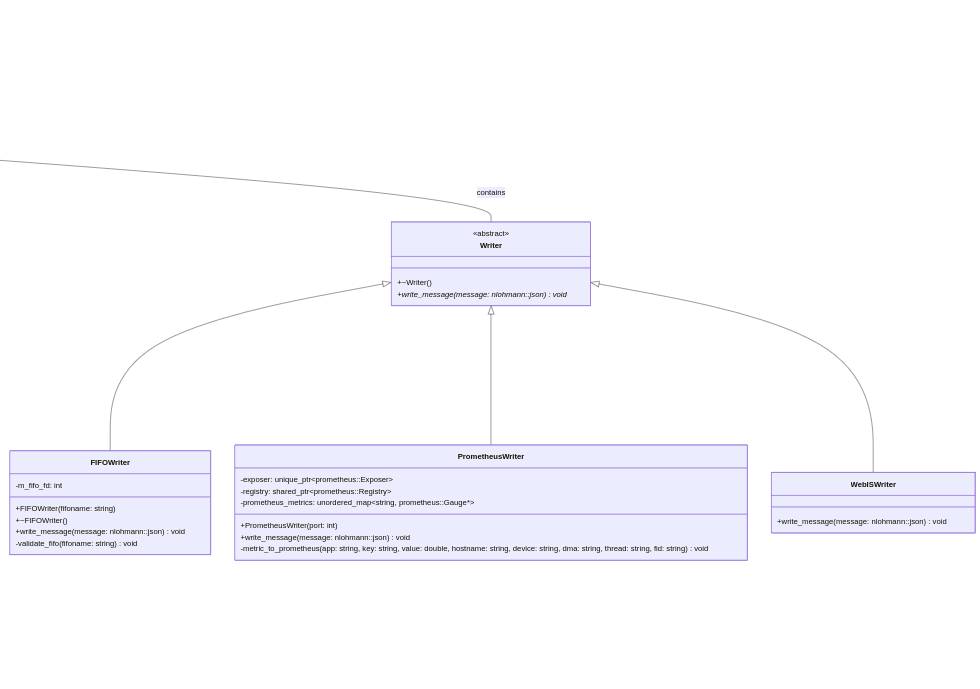
\includegraphics[width=\textwidth,height=\textheight,keepaspectratio]{images/appendix/complete-monitoring-uml-right.png}
    \caption{Complete Monitoring system UML diagram. Right part}
    \label{fig:complete-monitoring-uml-right}
\end{sidewaysfigure}
%\backmatter

%-------------------------------------------------------------------
% Bibliography
%-------------------------------------------------------------------

\printbibliography

\end{document}
